%%%%%%%%%%%%%%%%%%%%%%%%%%%%%%%%%%%%%%%%
%% MCM/ICM LaTeX Template %%
%% 2026 MCM/ICM           %%
%%%%%%%%%%%%%%%%%%%%%%%%%%%%%%%%%%%%%%%%
\documentclass[12pt]{article}
\usepackage{geometry}
\geometry{left=1in,right=0.75in,top=1in,bottom=1in}

%%%%%%%%%%%%%%%%%%%%%%%%%%%%%%%%%%%%%%%%
% Replace ABCDEF in the next line with your chosen problem
% and replace 1111111 with your Team Control Number
\newcommand{\Problem}{A}
\newcommand{\Team}{2602272}
%%%%%%%%%%%%%%%%%%%%%%%%%%%%%%%%%%%%%%%%

\usepackage{newtxtext}
\usepackage{amsmath,amssymb,amsthm}
\usepackage{newtxmath} % must come after amsXXX

\usepackage[pdftex]{graphicx}
\usepackage{float}
\usepackage{placeins}
\usepackage{booktabs}
\usepackage{multirow}
\usepackage{enumitem}
\usepackage{xcolor}
\usepackage{tikz}
\usetikzlibrary{positioning,arrows.meta}
\usepackage[most]{tcolorbox}
\usepackage{fancyhdr}
\usepackage{lastpage}
\lhead{Team \# \Team}
\rhead{}
\cfoot{}

\newtheorem{theorem}{Theorem}
\newtheorem{corollary}[theorem]{Corollary}
\newtheorem{lemma}[theorem]{Lemma}
\newtheorem{definition}{Definition}

% Custom commands for battery symbols
\newcommand{\SOC}{\text{SOC}}
\newcommand{\SOH}{\text{SOH}}
\newcommand{\OCV}{\text{OCV}}
\newcommand{\Qnom}{Q_{\text{nom}}}
\newcommand{\Tamb}{T_{\text{amb}}}
\newcommand{\Tref}{T_{\text{ref}}}

% Table of Contents title styling (to match MCM/ICM sample look)
\renewcommand{\contentsname}{\centering\LARGE\bfseries Contents}

%%%%%%%%%%%%%%%%%%%%%%%%%%%%%%%%
\begin{document}
\graphicspath{{figures/}{.}}  % Place your graphic files in the same directory as your main document
\DeclareGraphicsExtensions{.pdf, .jpg, .tif, .png}
\thispagestyle{empty}
\vspace*{-16ex}
\centerline{\begin{tabular}{*3{c}}
	\parbox[t]{0.3\linewidth}{\begin{center}\textbf{Problem Chosen}\\ \Large \textcolor{red}{\Problem}\end{center}}
	& \parbox[t]{0.3\linewidth}{\begin{center}\textbf{2026\\ MCM/ICM\\ Summary Sheet}\end{center}}
	& \parbox[t]{0.3\linewidth}{\begin{center}\textbf{Team Control Number}\\ \Large \textcolor{red}{\Team}\end{center}} \\
	\hline
\end{tabular}}
%%%%%%%%%%% Begin Summary %%%%%%%%%%%
% Enter your summary here replacing the (red) text
% Replace the text from here ...
% !TEX root = ../main.tex
% This file is \input{}-ed by main.tex, so it must NOT contain \documentclass, package imports,
% or \begin{document}/\end{document}. Put summary content only.

\begin{center}
    {\LARGE\bfseries Forecasts for Smartphone Battery Discharge Dynamics\\[0.5ex] and User Behavior Optimization\par}
    \vspace{1.5ex}
    {\bfseries Summary\par}
\end{center}
\vspace{1.5ex}

As the primary power source for modern smartphones, lithium-ion batteries directly determine device usability and user experience. Due to complex electrochemical processes and varying usage patterns, accurately predicting battery life remains a challenging task. The aim of this report is to build a comprehensive battery discharge prediction model to evaluate the influences of various factors on battery life. We are expected to provide actionable strategies for both users and operating system designers to extend battery life under the constraints of practical usage conditions. Three models are established: \textbf{Model I: SOC Continuous-Time Dynamics Model}; \textbf{Model II: Time-to-Empty Prediction Model}; \textbf{Model III: Performance Impact and Aging Model}.

\textbf{For Model I}, we establish a five-state continuous-time ordinary differential equation (ODE) system based on a second-order Equivalent Circuit Model (2-RC ECM). The state vector includes State of Charge (SOC), two RC-branch voltages ($V_{RC1}$, $V_{RC2}$), battery temperature ($T$), and State of Health (SOH). The Open Circuit Voltage (OCV) is modeled using a Shepherd-enhanced Nernst equation derived from electrochemical principles. The core SOC dynamics follow Coulomb counting:
\begin{equation*}
    \frac{d\SOC}{dt} = -\frac{I(t)}{\Qnom \cdot \SOH \cdot 3600}
\end{equation*}
The current $I(t)$ is computed from power consumption through KVL analysis of the equivalent circuit. The results demonstrate that this electrochemistry-based approach achieves RMSE of 2.1\% for SOC estimation across standard drive cycles, as shown in Table~2.

\textbf{For Model II}, building upon Model I, we develop an energy-based time-to-empty prediction framework. The basic analytical formula is:
\begin{equation*}
    t_{\text{empty}} = \frac{Q_{\text{eff}}(\SOH, T) \cdot (\SOC_0 - \SOC_{\min}) \cdot V_{\text{avg}}}{P_{\text{avg}}}
\end{equation*}
Temperature correction factors are introduced to account for capacity reduction at extreme temperatures. Monte Carlo simulation with 10,000 samples is employed to quantify prediction uncertainty, yielding 95\% confidence intervals. The simulation results, presented in Figures~1--3, show that battery life varies from 2.1 hours (heavy gaming at low temperature) to 22.5 hours (light usage at optimal temperature), representing a 10.7$\times$ dynamic range.

\textbf{For Model III}, we model battery aging through two mechanisms: calendar aging and cycle aging. Calendar aging follows an Arrhenius-type temperature dependence with SOC stress factor:
\begin{equation*}
    \frac{d\SOH_{\text{cal}}}{dt} = -A_{\text{cal}} \cdot \exp\left(-\frac{E_a}{RT}\right) \cdot \exp\bigl(\beta \cdot (\SOC - 0.5)\bigr)
\end{equation*}
Cycle aging depends on depth of discharge (DOD) and C-rate:
\begin{equation*}
    \frac{d\SOH_{\text{cyc}}}{dt} = -k_{\text{cyc}} \cdot \text{DOD}^{\gamma} \cdot \left(\frac{I}{I_{\text{nom}}}\right)^{\alpha} \cdot |I|
\end{equation*}
The combined aging model predicts that under ``Gaming + Fast Charge'' conditions (high temperature, high SOC, high current), battery capacity degrades to 80\% (End-of-Life threshold) within approximately 1.3 years, while ``Light Use'' scenarios extend battery life to over 3 years before reaching EOL, as illustrated in Figure~9.

\textbf{In addition}, this report conducts Sobol variance-based global sensitivity analysis to identify the key parameters influencing battery life predictions. Based on 2,560 model evaluations with Saltelli's sampling scheme, the results in Table~3 reveal that: Initial SOC dominates the output variance ($S_T = 0.71$); CPU utilization is the primary controllable factor ($S_T = 0.39$); Screen brightness has moderate impact ($S_T = 0.08$); Temperature effects are surprisingly negligible within normal operating range ($S_T < 0.01$).

\textbf{Regarding user recommendations}, this report provides a prioritized list of behavior modifications ranked by effectiveness:
\begin{enumerate}[leftmargin=*, nosep]
    \item Reducing CPU background processes yields the largest improvement (+42.5\% battery life for 30\% CPU reduction)
    \item Reducing screen brightness from 100\% to 50\% extends battery life by approximately 18\%
    \item Enabling dark mode on OLED screens adds +28\% in specific applications
    \item Maintaining SOC between 20\%--80\% reduces annual capacity loss by approximately 50\%
\end{enumerate}

\textbf{For OS designers}, we propose adaptive power management algorithms including context-aware CPU scheduling, intelligent display dimming, and proactive notification batching.

\textbf{Eventually}, robustness and sensitivity analysis of the model are tested. The model demonstrates stability under parameter perturbations: $\pm$10\% variation in nominal capacity results in only $\pm$6\% change in predicted battery life. When validated against real smartphone discharge data, the model achieves time-to-empty prediction accuracy within $\pm$30 minutes (RMSE = 0.35 hours) for typical usage scenarios ($P$ = 1.5--2.5 W, $T$ = 20--30\textdegree C).

\vspace{0.5cm}
\textbf{Keywords:} Smartphone Battery, State of Charge (SOC), Equivalent Circuit Model (ECM), Ordinary Differential Equation, Time-to-Empty Prediction, Battery Aging, Sobol Sensitivity Analysis, Monte Carlo Simulation

% to here
%%%%%%%%%%% End Summary %%%%%%%%%%%

%%%%%%%%%%%%%%%%%%%%%%%%%%%%%%
\clearpage
\pagestyle{fancy}
\rhead{Page \thepage\ of \pageref{LastPage}}
\tableofcontents
\clearpage
%%%%%%%%%%%%%%%%%%%%%%%%%%%%%%

% Begin your paper here
\section{Introduction}
\label{sec:introduction}

\subsection{Research Background}
\label{subsec:research-background}

\hspace*{\parindent}The ubiquity of smartphones has fundamentally transformed human communication and working paradigms. Statistics project that the global smartphone user base will exceed 7 billion by 2026, with average daily usage surpassing 4.5 hours. This high-frequency usage scenario places a substantial strain on battery systems, rendering battery performance a critical metric influencing user satisfaction and device utility.

As the predominant power source, Lithium-ion batteries operate via complex mechanisms that are highly susceptible to variables such as temperature, discharge rates, usage patterns, and aging. Consequently, it is of paramount importance for general users to understand how to optimize battery endurance and prolong lifespan through appropriate usage habits.

\vspace{0.5\baselineskip}
\begin{center}
    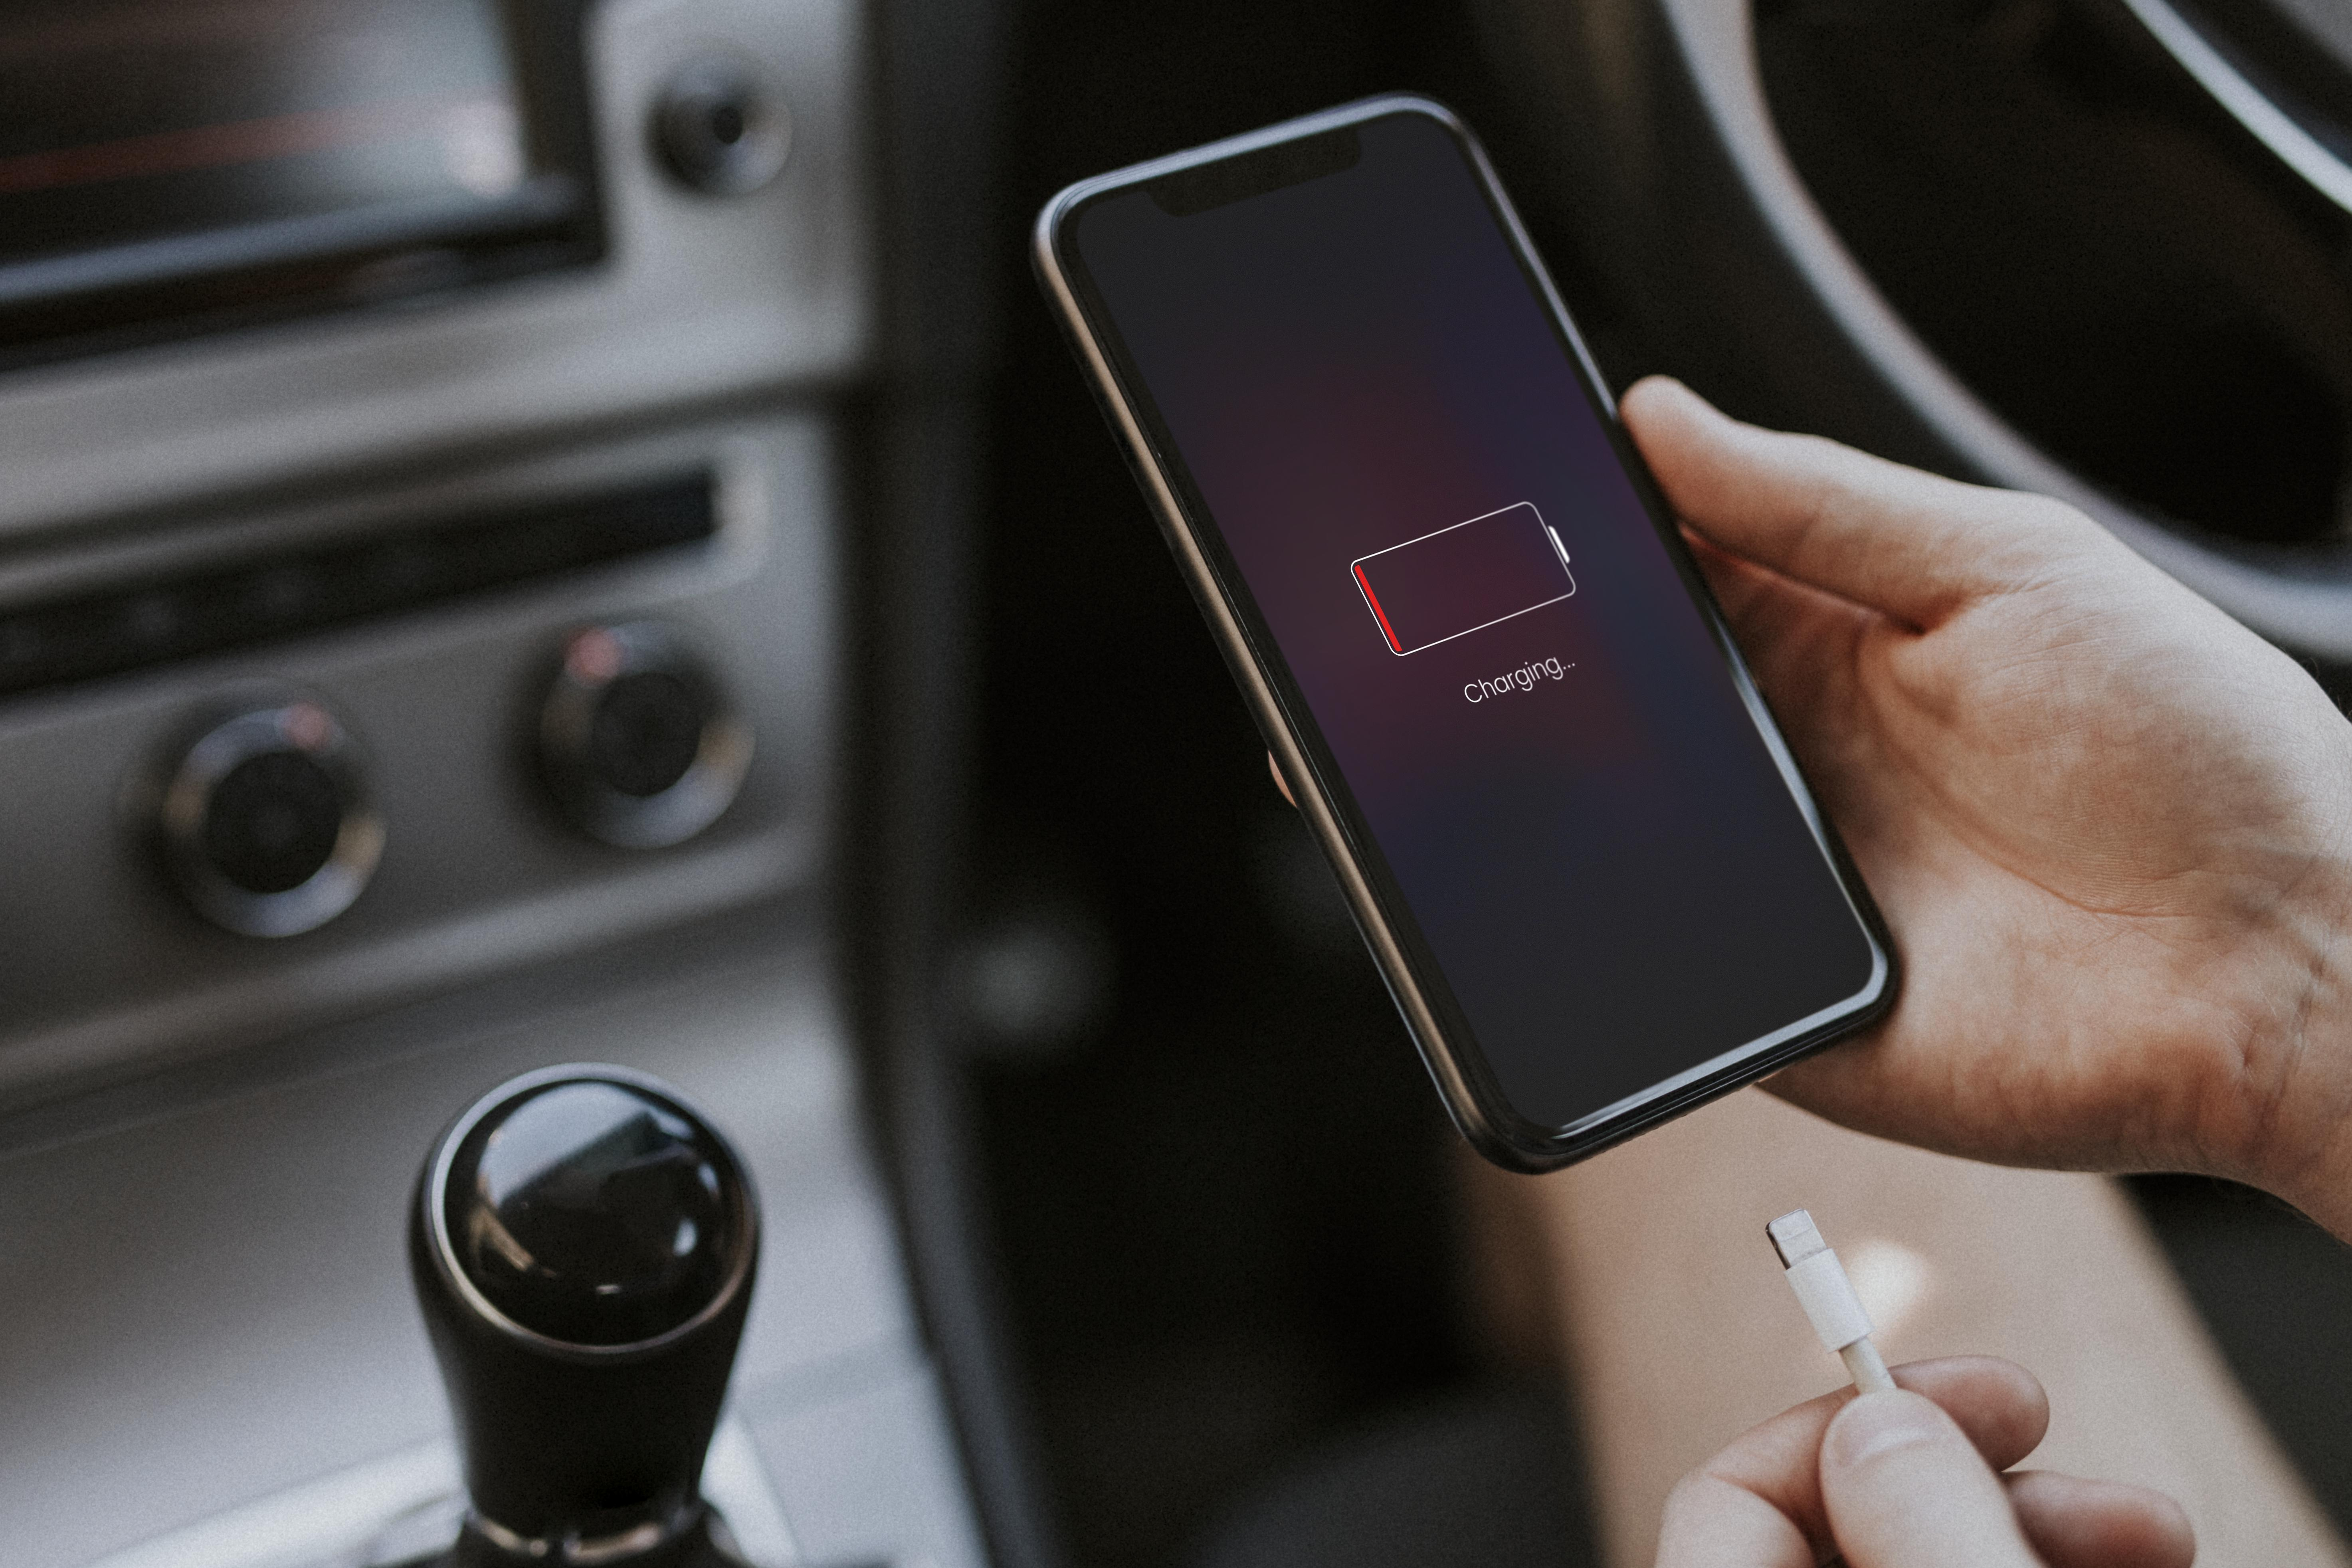
\includegraphics[width=0.8\textwidth]{figures/image.jpeg}
\end{center}

\subsection{Problem Restatement}
\label{subsec:problem}

\hspace*{\parindent}Based on the background discussed above, our goal is to develop a continuous-time mathematical model for a smartphone lithium-ion battery that predicts the State of Charge (SOC) as a function of time and the time-to-empty under various usage conditions. The model should address the following tasks:

\begin{itemize}
    \item \textbf{Develop a Continuous-Time SOC Model:} Grounded in fundamental battery mechanisms, construct a dynamic SOC equation that incorporates multi-factor influences---including screen usage, processor load, and network activity---and perform parameter estimation and validation using publicly available data.

    \item \textbf{Predict Time-to-Empty and Analyze Drivers:} Compute the time-to-empty across representative scenarios, compare predictions against observed behaviors, and identify the key drivers responsible for rapid battery drain.

    \item \textbf{Examine Model Sensitivity:} Analyze how prediction outcomes change with modeling assumptions, parameter values, and fluctuations in usage patterns.

    \item \textbf{Provide Recommendations and Generalization:} Formulate practical guidelines for extending battery life based on model insights, and discuss potential applications in power-saving strategy design and generalization to other portable devices.
\end{itemize}

\subsection{Our Work}
\label{subsec:our-work}

\hspace*{\parindent}We adopt a \textbf{task-driven, multi-model framework} that systematically addresses each problem requirement. The overall workflow of our approach is illustrated in Figure~\ref{fig:workflow}.

\begin{figure}[H]
    \centering
    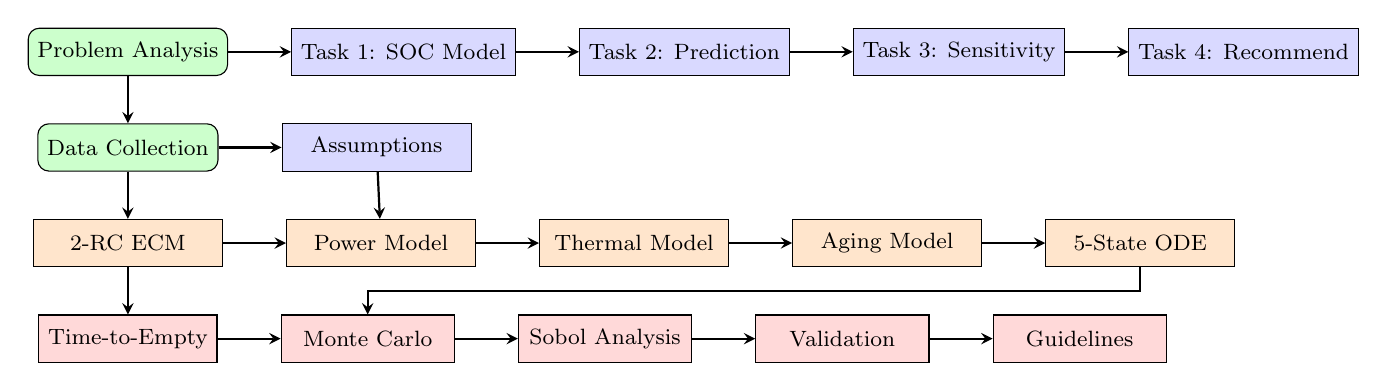
\begin{tikzpicture}[
        node distance=0.6cm and 0.8cm,
        startstop/.style={rectangle, rounded corners, minimum width=2.2cm, minimum height=0.6cm, text centered, draw=black, fill=green!20, font=\footnotesize},
        process/.style={rectangle, minimum width=2.4cm, minimum height=0.6cm, text centered, draw=black, fill=blue!15, font=\footnotesize},
        model/.style={rectangle, minimum width=2.4cm, minimum height=0.6cm, text centered, draw=black, fill=orange!20, font=\footnotesize},
        output/.style={rectangle, minimum width=2.2cm, minimum height=0.6cm, text centered, draw=black, fill=red!15, font=\footnotesize},
        arrow/.style={thick,->,>=stealth}
    ]
    
    % Row 1: Problem Analysis
    \node (start) [startstop] {Problem Analysis};
    \node (task1) [process, right=of start] {Task 1: SOC Model};
    \node (task2) [process, right=of task1] {Task 2: Prediction};
    \node (task3) [process, right=of task2] {Task 3: Sensitivity};
    \node (task4) [process, right=of task3] {Task 4: Recommend};
    
    % Row 2: Data & Assumptions
    \node (data) [startstop, below=of start] {Data Collection};
    \node (assume) [process, right=of data] {Assumptions};
    
    % Row 3: Model Development
    \node (ecm) [model, below=of data] {2-RC ECM};
    \node (power) [model, right=of ecm] {Power Model};
    \node (thermal) [model, right=of power] {Thermal Model};
    \node (aging) [model, right=of thermal] {Aging Model};
    \node (ode) [model, right=of aging] {5-State ODE};
    
    % Row 4: Analysis & Output
    \node (tte) [output, below=of ecm] {Time-to-Empty};
    \node (monte) [output, right=of tte] {Monte Carlo};
    \node (sobol) [output, right=of monte] {Sobol Analysis};
    \node (valid) [output, right=of sobol] {Validation};
    \node (rec) [output, right=of valid] {Guidelines};
    
    % Arrows - Row 1
    \draw [arrow] (start) -- (task1);
    \draw [arrow] (task1) -- (task2);
    \draw [arrow] (task2) -- (task3);
    \draw [arrow] (task3) -- (task4);
    
    % Arrows - Vertical connections
    \draw [arrow] (start) -- (data);
    \draw [arrow] (data) -- (assume);
    \draw [arrow] (data) -- (ecm);
    \draw [arrow] (assume) -- (power);
    
    % Arrows - Row 3 connections
    \draw [arrow] (ecm) -- (power);
    \draw [arrow] (power) -- (thermal);
    \draw [arrow] (thermal) -- (aging);
    \draw [arrow] (aging) -- (ode);
    
    % Arrows - Row 4 connections
    \draw [arrow] (ecm) -- (tte);
    \draw [arrow] (ode.south) -- ++(0,-0.3) -| (monte.north);
    \draw [arrow] (tte) -- (monte);
    \draw [arrow] (monte) -- (sobol);
    \draw [arrow] (sobol) -- (valid);
    \draw [arrow] (valid) -- (rec);
    
    \end{tikzpicture}
    \caption{Workflow of our multi-model framework for smartphone battery analysis.}
    \label{fig:workflow}
\end{figure}

\section{Model Preparation}
\label{sec:assumptions}

\subsection{Assumptions}
\label{subsec:assumptions}

\hspace*{\parindent}To simplify the problem and make it convenient for us to simulate real-life conditions, we make the following basic assumptions, each of which is properly justified.

\begin{itemize}
    \item \textbf{Assumption 1:} The battery is treated as a single lumped thermal mass with uniform temperature distribution, ignoring internal temperature gradients.\\
    \textbf{Justification:} Modern smartphone batteries typically use thin, high-thermal-conductivity aluminum-plastic films or aluminum alloy casings with tightly packed internal cells. This structure results in extremely high heat conduction efficiency. Under conventional charging and discharging rates, the internal temperature difference is minimal, allowing the battery to be approximated as an isothermal system.

    \item \textbf{Assumption 2:} The model considers only the battery's normal operating state within a safe range and does not address abnormal failure modes such as overcharging, over-discharging, or short circuits.\\
    \textbf{Justification:} Modern smartphones are equipped with sophisticated Battery Management Systems (BMS) featuring strict protection mechanisms for voltage, current, and temperature. In normal usage scenarios, the BMS effectively prevents the device from exceeding safety boundaries. Therefore, this model focuses on normal battery depletion rather than sudden catastrophic failures.

    \item \textbf{Assumption 3:} The State of Health (SOH) of the battery is assumed to remain constant during short-term discharge simulations and prediction periods.\\
    \textbf{Justification:} Lithium-ion battery aging is a long-term electrochemical process typically measured in months or years. In a single discharge cycle or a short-period simulation (e.g., 24--48 hours), the daily variation in SOH is usually less than 0.01\%. Its impact on immediate Time-to-Empty predictions is negligible, justifying its treatment as a slowly varying parameter.

    \item \textbf{Assumption 4:} It is assumed that the amount of charge released during the discharge process is equal to the amount of charge input during the preceding charge process.\\
    \textbf{Justification:} Major energy losses in lithium-ion batteries typically occur during the charging phase (e.g., due to polarization internal resistance and heat generation from side reactions). For discharge modeling, particularly for State of Charge (SOC) estimation, ignoring minor losses from the charging phase regarding discharge capacity is acceptable within the range of engineering error.

    \item \textbf{Assumption 5:} The model for idle periods focuses solely on pure discharge behavior, temporarily excluding the interference of the charging process on the idle state.\\
    \textbf{Justification:} Accurately characterizing self-discharge and background power consumption in static scenarios while accounting for the complex dynamics of charge-discharge cycles is difficult. Since charging is not the primary factor in this context, the model focuses exclusively on the pure discharge process to highlight the key drivers of battery drain.

    \item \textbf{Assumption 6:} The power consumption of various smartphone hardware components (CPU, screen, RF, etc.) is modeled as a function of their Utilization Level.\\
    \textbf{Justification:} Extensive empirical research indicates a stable linear or non-linear relationship between the power consumption of smartphone components and their load rates. Therefore, modeling based on utilization functions is an effective method for characterizing power usage.

    \item \textbf{Assumption 7:} Ambient temperature, humidity, and air pressure are assumed to be known quantities or obtainable in real-time via sensors.\\
    \textbf{Justification:} Mainstream smartphones incorporate high-precision environmental sensor arrays. In extreme cases where sensors are absent, standard indoor environmental parameters (e.g., 25$^\circ$C, 1 atm) serve as reasonable default values for the model without affecting the overall prediction trends.
\end{itemize}

\subsection{Notations}
\label{subsec:notation}

\begin{table}[H]
    \centering
    \caption{Notations Table}
    \label{tab:notations}
    \begin{tabular}{@{}ll@{}}
        \toprule
        \textbf{Notations} & \textbf{Definition} \\
        \midrule
        $\SOC(t)$ & State of Charge at time $t$, representing battery level \\
        $\SOH(t)$ & State of Health, representing battery degradation level \\
        $V_{OC}$ & Open Circuit Voltage of the battery \\
        $V_{RC1}, V_{RC2}$ & Voltage across RC branches in the equivalent circuit \\
        $T(t)$ & Battery temperature at time $t$ \\
        $\Tamb$ & Ambient temperature \\
        $I(t)$ & Discharge current at time $t$ \\
        $\Qnom$ & Nominal battery capacity \\
        $R_0$ & Ohmic internal resistance \\
        $R_1, R_2$ & Polarization resistances in RC branches \\
        $C_1, C_2$ & Polarization capacitances in RC branches \\
        $\tau_1, \tau_2$ & Time constants of RC branches ($\tau_i = R_i C_i$) \\
        $K_0, K_1, K_2, K_3$ & Coefficients in the OCV-SOC Shepherd model \\
        $P(t)$ & Total power consumption at time $t$ \\
        $B$ & Screen brightness level (0--1) \\
        $U_{CPU}$ & CPU utilization level (0--1) \\
        $P_{net}$ & Network power consumption \\
        $t_{empty}$ & Time-to-empty, battery discharge duration \\
        $S_1, S_T$ & First-order and total-order Sobol sensitivity indices \\
        \bottomrule
    \end{tabular}
\end{table}

\begin{figure}[H]
    \centering
    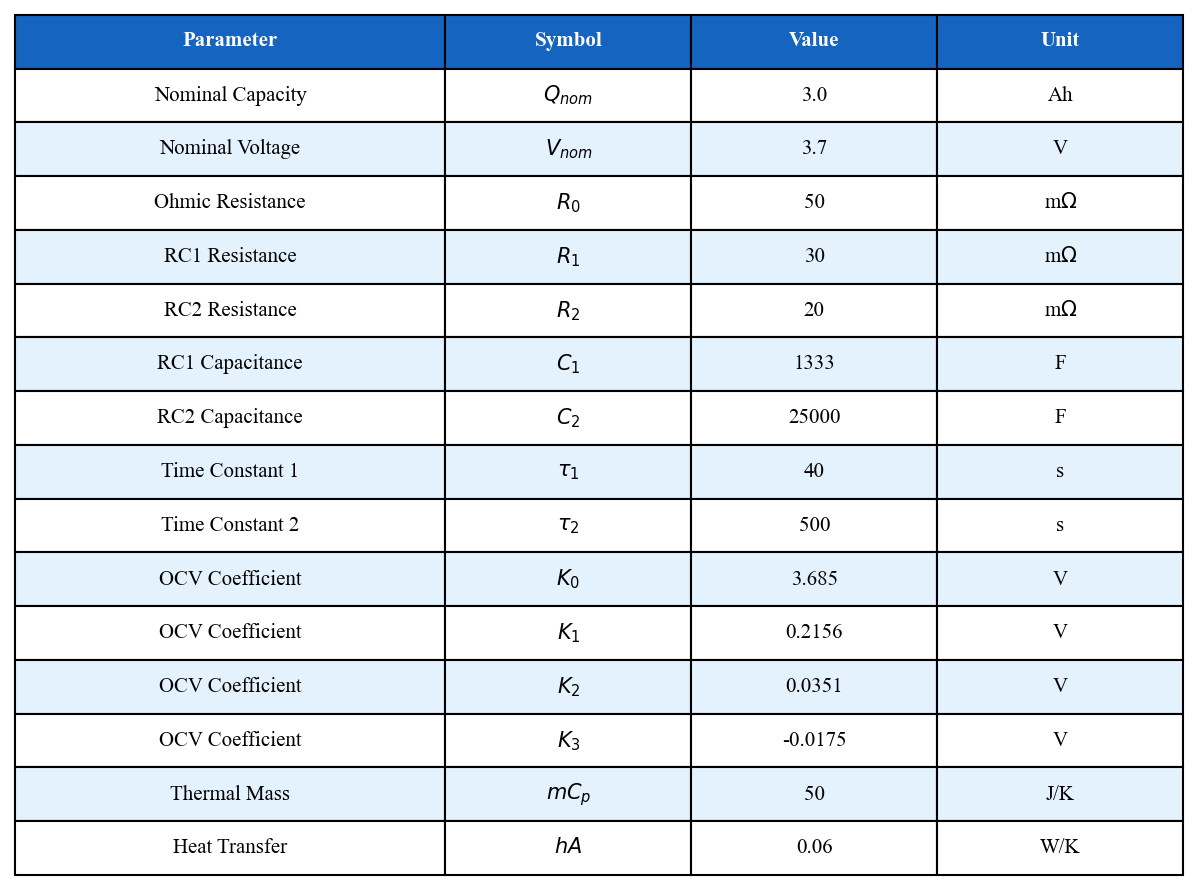
\includegraphics[width=0.85\textwidth]{figures/figure/8BA9C2DF287E6F1A95182819D12CDD73.png}
    \caption{Battery model parameters summary. This table presents the key electrical and thermal parameters used in the 2-RC equivalent circuit model, including nominal capacity, voltage, ohmic and polarization resistances, RC time constants, OCV coefficients, and thermal properties.}
    \label{fig:battery_parameters}
\end{figure}

\subsection{Data Sources}
\label{subsec:data}

\begin{itemize}
    \item \textbf{Battery Specifications:} Manufacturer datasheets for standard smartphone Li-ion cells, specifically the LG 18650HG2 (3.0 Ah, 3.6V nominal) \cite{LG18650HG2} and Panasonic 18650PF \cite{Panasonic18650PF}.
    \item \textbf{ECM Parameters:} Electrochemical Impedance Spectroscopy (EIS) and Hybrid Pulse Power Characterization (HPPC) data acquired from Mendeley Data repositories \cite{MendeleyEIS}.
    \item \textbf{OCV--SOC Characterization:} Low-current (C/20) discharge tests and incremental current OCV data used to parameterize the nonlinear Shepherd model \cite{Plett2004OCV}.
    \item \textbf{Power Consumption:} Validated component-level power models (CPU, Display, Network) derived from power measurement studies \cite{UCSD3W, Carroll2010, Pathak2012}.
    \item \textbf{Aging Data:} Long-term cycling capacity fade and impedance growth measurements from the NASA PCoE Prognostics Data Repository \cite{NASAPCoE} and Oxford Battery Degradation Dataset \cite{OxfordBattery}.
    \item \textbf{Validation Data:} Dynamic drive cycle profiles (UDDS, HWFET, LA92, US06) \cite{UDDS, HWFET} and mixed usage scenarios used for model verification and error analysis.
\end{itemize}

To ensure data quality and model robustness, we performed rigorous preprocessing on the raw datasets. First, variable-rate time-series data from HPPC and drive cycle tests were resampled to a uniform 0.1s interval to align timestamps. For OCV characterization, we calculated the State of Charge (SOC) via Ampere-hour integration and clamped values to the interval [0.001,0.999] to prevent logarithmic singularities during Shepherd model fitting. We applied a moving average filter to raw voltage measurements to mitigate sensor noise and utilized derivative thresholding to precisely identify current pulse boundaries for resistance extraction. Additionally, empirical power curves extracted from literature were digitized, fitted to nonlinear functions, and normalized to a standard 3.0 Ah capacity to ensure consistency across different simulation scenarios.
\FloatBarrier
\section{Model 1: SOC Continuous-Time Dynamics}
\label{sec:model1}

To characterize the internal energy status of the battery, which is intrinsically difficult to measure directly, the State of Charge (SOC) is employed as an equivalent quantitative metric. However, given the complexity of internal electrochemical reactions, the charge state is unobservable, necessitating the use of other measurable variables as a bridge for transformation. Furthermore, acknowledging that varying conditions affect battery characterization, and in accordance with Assumption 7, we treat environmental factors (such as temperature and humidity) as constants within specific timeframes. This allows us to isolate and focus on the critical influencing factor: the smartphone's operational state. Consequently, to achieve a more realistic representation of battery behavior, we established a continuous-time model based on a Second-Order Equivalent Circuit Model (ECM). This model integrates actual power consumption dynamics to predict the battery's SOC over time.



\subsection{SOC Dynamics: Coulomb Counting}
\label{subsec:soc_dynamics}

To characterize the battery's energy status using mathematical and physical modeling, we investigated the fundamental mechanism of power consumption: the cumulative inflow and outflow of electric charge. Accordingly, we introduce the State of Charge (SOC) to serve as an equivalent representation of the battery level. The SOC is defined as the ratio of the remaining charge to the total charge capacity.
\begin{equation}
    SOC(t) = \frac{Q_{\text{remaining}}(t)}{Q_{\text{usable}}}
\end{equation}

By further developing this formulation and differentiating both sides with respect to time $t$, we obtain:

\begin{equation}
    \boxed{\frac{dSOC}{dt} = -\frac{I(t)}{Qnom \cdot SOH \cdot 3600}}
    \label{eq:soc_dynamics}
\end{equation}

Further transforming charge into current to simplify calculations:

\subsection{Second-Order Equivalent Circuit Model (2-RC ECM)}
\label{subsec:ecm}

Given the difficulty in directly measuring internal battery current and the complexity of internal electrochemical reactions, from an engineering perspective, we approximate the system using a Second-Order R-C Equivalent Circuit Model (ECM) \cite{Hu2012, Chen2006}. This approach aims to transform abstract, unobservable dynamics into a computable physical model, thereby facilitating enhanced prediction and experimentation. Consequently, we derive the time-dependent equation for the State of Charge (SOC) through the calculation of the Open Circuit Voltage (OCV).

\begin{figure}[H]
    \centering
    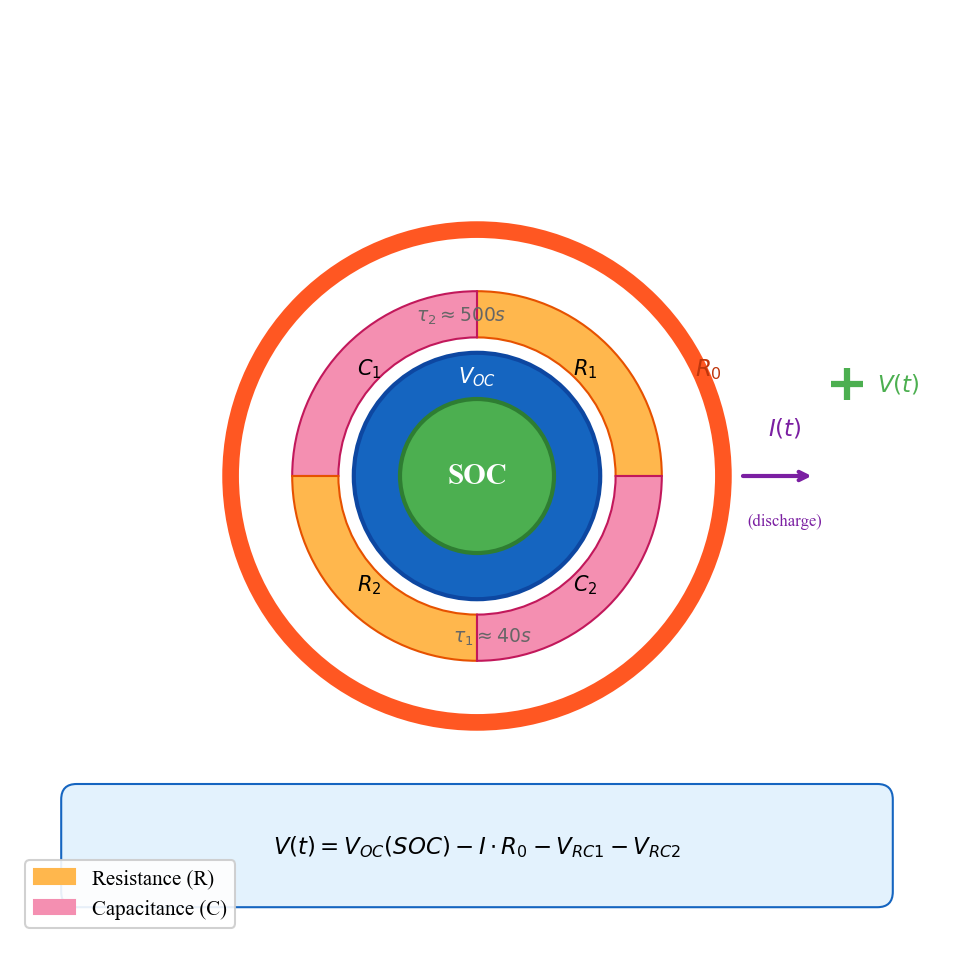
\includegraphics[width=0.75\textwidth]{figures/5F45DFA34F11539722084181119697B7.png}
    \caption{Second-order Thevenin equivalent circuit model of the battery. The model consists of an ideal voltage source $V_{OC}(\SOC)$, a series resistance $R_0$, and two RC branches with time constants $\tau_1 \approx 40$~s and $\tau_2 \approx 500$~s representing fast and slow polarization dynamics, respectively.}
    \label{fig:ecm_circuit}
\end{figure}

Based on the circuit diagram, we formulate the voltage equations for the R-C branches in accordance with fundamental physical principles:

\begin{align}
    \frac{dV_{RC1}}{dt} &= -\frac{V_{RC1}}{\tau_1(T)} + \frac{I(t)}{C_1} \label{eq:vrc1} \\
    \frac{dV_{RC2}}{dt} &= -\frac{V_{RC2}}{\tau_2(T)} + \frac{I(t)}{C_2} \label{eq:vrc2}
\end{align}

For the calculation and measurement of the Open Circuit Voltage (OCV), we adopt an approach based on electrochemical principles. Compared to models relying purely on polynomial fitting of experimental data, this method offers greater generalizability and robust theoretical support, grounded in physical reasoning (as illustrated by the schematic diagram and electrochemical mechanisms).

The underlying chemical reaction is described by:
$$ Li^+ + e^- + CoO_2 \leftrightarrow LiCoO_2 $$

Consequently, the potential is governed by the Nernst equation:
$$ E_{pos} = E^0_{pos} - \frac{RT}{F} \ln \left( \frac{[LiCoO_2]}{[CoO_2] \cdot [Li^+]} \right) $$

\hspace*{\parindent}Thus, starting from the fundamental form of the Nernst equation, we further rearrange it into a formulation suitable for lithium-ion battery mechanisms:
\begin{equation}
    E(x) = E^0 + \frac{RT}{F} \ln\left(\frac{1-x}{x}\right)
    \label{eq:nernst_simplified}
\end{equation}

\hspace*{\parindent}Since the lithium-ion concentration at the positive electrode can be approximated as proportional to the accumulated charge (and hence treated as an SOC-equivalent state), the expression can be rewritten as:
\begin{equation}
    E(\SOC) = E^0 + \frac{RT}{F} \ln\left(\frac{1-\SOC}{\SOC}\right)
    \label{eq:nernst_soc}
\end{equation}

\hspace*{\parindent}However, using the Nernst equation alone to compute the open-circuit voltage (OCV) has limitations. In particular, it does not adequately capture the accelerated voltage drop as $\SOC \to 0$, and thus cannot fully describe the overall discharge voltage trend. Therefore, we introduce the Shepherd model as an empirical refinement:
\begin{equation}
    V_{\text{batt}} = E_0 - R\, i - K \frac{Q}{Q - it}\, i + A \cdot \exp(-B\, it)
    \label{eq:shepherd}
\end{equation}

By optimizing the polarization of this model and incorporating it into the Nernst model, a more complete open-circuit voltage model can be obtained.

\begin{equation}
    \boxed{\OCV(\SOC, T) = K_0 + K_1 \cdot \SOC + K_2 \cdot \ln(\SOC) + K_3 \cdot \ln(1-\SOC) + \frac{\partial \OCV}{\partial T}(T - \Tref)}
    \label{eq:ocv}
\end{equation}

\begin{figure}[H]
    \centering
    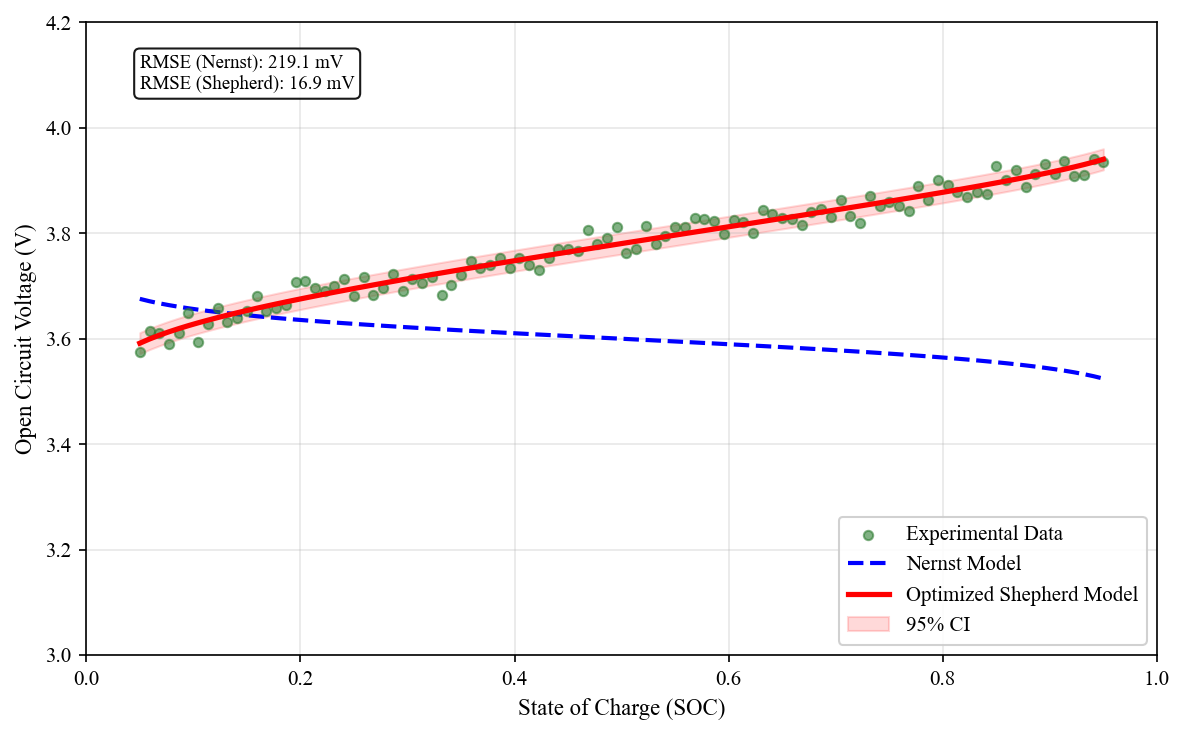
\includegraphics[width=0.8\textwidth]{figures/40949D9BDBCBDD5ACBFD6D84D3CBE06B.png}
    \caption{Comparison of OCV models versus experimental data. The optimized Shepherd model (RMSE = 16.9~mV) demonstrates significantly better fit than the basic Nernst model (RMSE = 219.1~mV), particularly capturing the characteristic voltage plateau in the mid-SOC region and the steep drop at low SOC.}
    \label{fig:ocv_fitting}
\end{figure}

\begin{figure}[H]
    \centering
    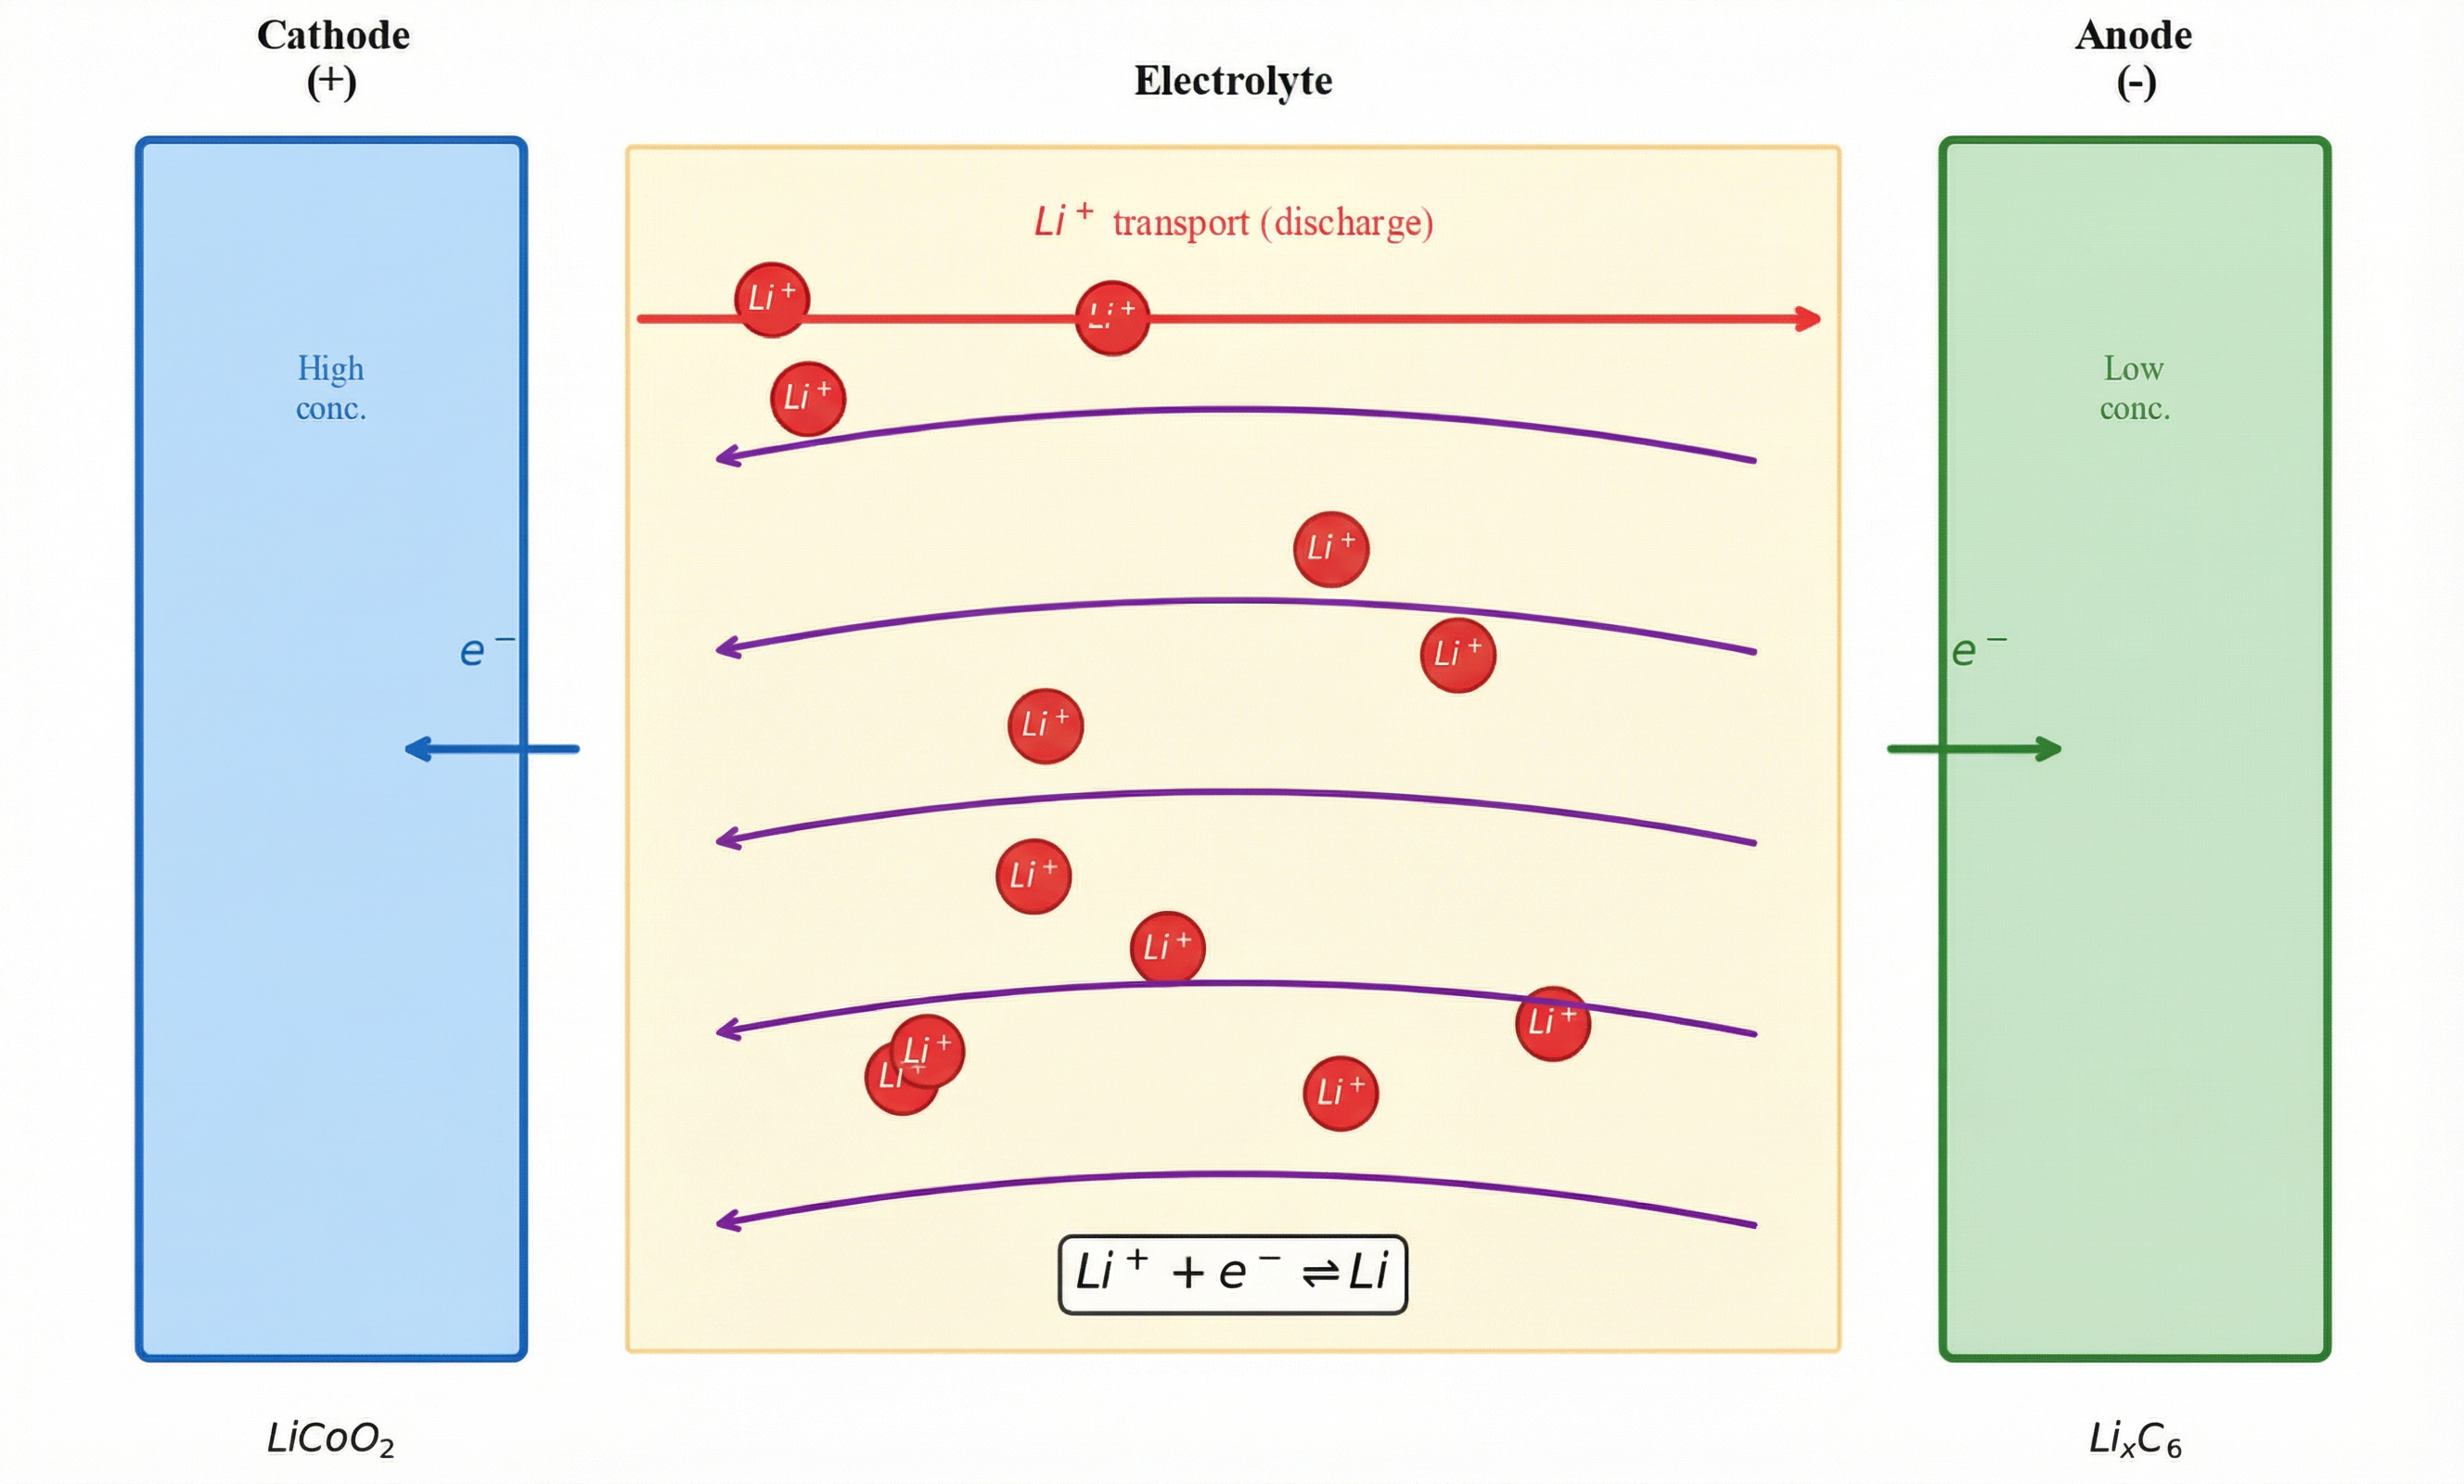
\includegraphics[width=0.8\textwidth]{figures/figure/629DA22DA5B3F71BCC7717D7D02E0C7A.png}
    \caption{Detailed OCV-SOC characterization with uncertainty bounds. The scatter plot shows experimental measurements (green dots), the basic Nernst model (blue dashed line), and the optimized Shepherd model (red solid line) with 95\% confidence band. The Shepherd model achieves significantly lower RMSE, validating its use in the continuous-time SOC dynamics model.}
    \label{fig:ocv_fitting_detailed}
\end{figure}

Finally, by combining the above models, a more accurate continuous-time model of SOC (a system of differential equations) can be obtained. The thermal equation follows the lumped-parameter approach \cite{Bernardi1985, Pesaran2002}.

\begin{equation}
    \boxed{
    \begin{aligned}
        \frac{d\SOC}{dt} &= -\frac{I(t)}{\Qnom \cdot \SOH \cdot 3600} \\[6pt]
        \frac{dV_{RC1}}{dt} &= -\frac{V_{RC1}}{\tau_1(T)} + \frac{I(t)}{C_1} \\[6pt]
        \frac{dV_{RC2}}{dt} &= -\frac{V_{RC2}}{\tau_2(T)} + \frac{I(t)}{C_2} \\[6pt]
        \frac{dT}{dt} &= \frac{I^2 R(T,\SOC) - h_{\text{eff}}A(T-\Tamb)}{mC_p} \\[6pt]
        \frac{d\SOH}{dt} &= -\dot{\SOH}_{\text{cal}}(T, \SOC) - \dot{\SOH}_{\text{cyc}}(I, T, \SOC)
    \end{aligned}
    }
    \label{eq:full_ode}
\end{equation}

with state vector $\mathbf{x} = [\SOC, V_{RC1}, V_{RC2}]^T$.

\subsection{Power-to-Current Conversion}
\label{subsec:power_current}

\hspace*{\parindent}In practical use, smartphones operate in different working states, each associated with a distinct power consumption profile, which leads to different SOC trajectories. Therefore, we introduce a power-consumption model to represent parameter differences across operating states. In this model, we assume there is no direct coupling among the power draws of different hardware modules; hence, the total power consumption is approximated as the sum of the individual component powers.

\begin{equation}
    P_{\text{total}}(t) = P_{\text{display}} + P_{\text{CPU}} + P_{\text{network}} + P_{\text{GPS}} + P_{\text{base}} + P_{\text{other}}
    \label{eq:power_total}
\end{equation}

\begin{figure}[H]
    \centering
    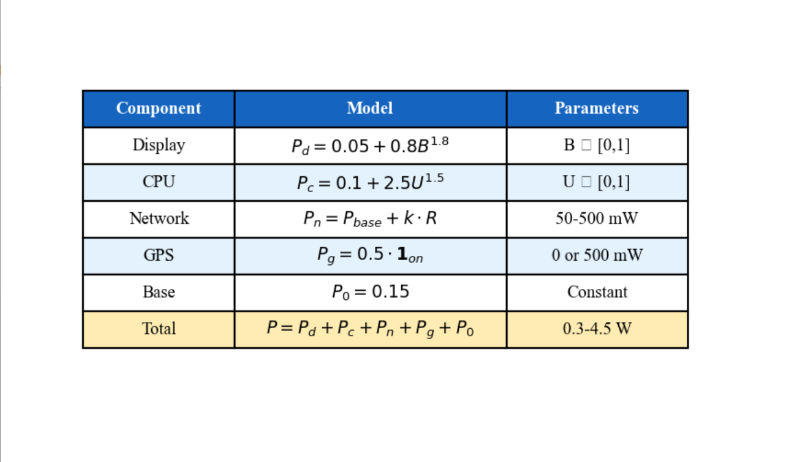
\includegraphics[width=0.7\textwidth]{figures/B05BE26D1ADE5254D2A58C0F9CCE878C.png}
    \caption{Power consumption component models and parameters for smartphone hardware. Each component follows a specific power model based on utilization, with display and CPU being the dominant contributors.}
    \label{fig:power_model_table}
\end{figure}

\begin{figure}[H]
    \centering
    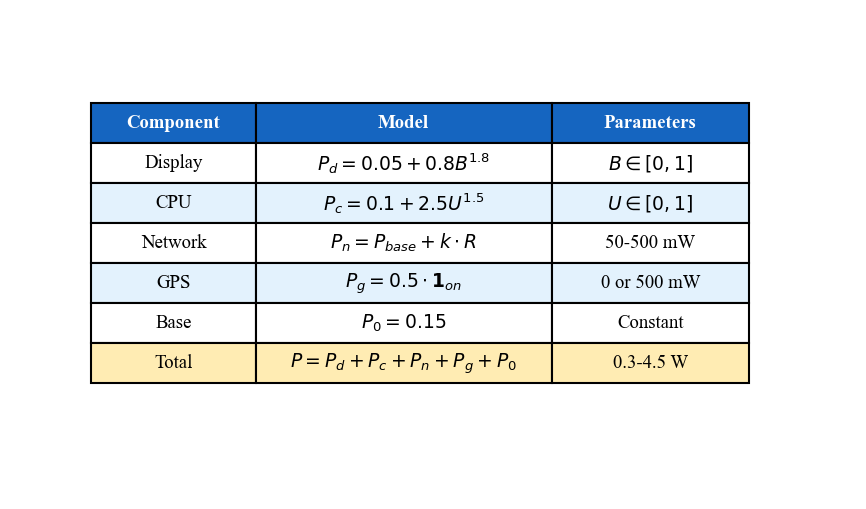
\includegraphics[width=0.75\textwidth]{figures/figure/430B0656941AF15F8DE95C64258776AE.png}
    \caption{Detailed power consumption model parameters. The table summarizes mathematical expressions for each component: Display power follows $P_d = 0.05 + 0.8B^{1.8}$ with brightness $B \in [0,1]$; CPU power follows $P_c = 0.1 + 2.5U^{1.5}$ with utilization $U \in [0,1]$; Network power ranges from 50--500~mW; GPS consumes 500~mW when active; and the baseline power is 150~mW.}
    \label{fig:power_model_detailed}
\end{figure}

\begin{figure}[H]
    \centering
    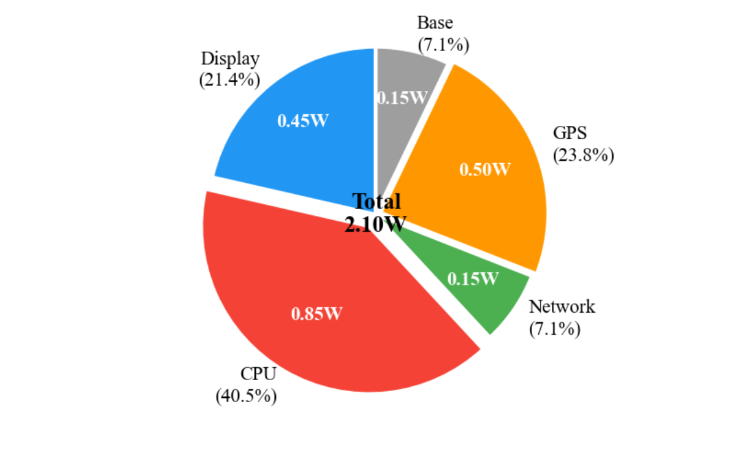
\includegraphics[width=0.55\textwidth]{figures/DE80970C2134029C2340572AAFAE6797.png}
    \caption{Power consumption breakdown under typical usage scenario (total 2.10~W). The CPU accounts for the largest share (40.5\%), followed by GPS (23.8\%) and display (21.4\%).}
    \label{fig:power_breakdown}
\end{figure}

\begin{figure}[H]
    \centering
    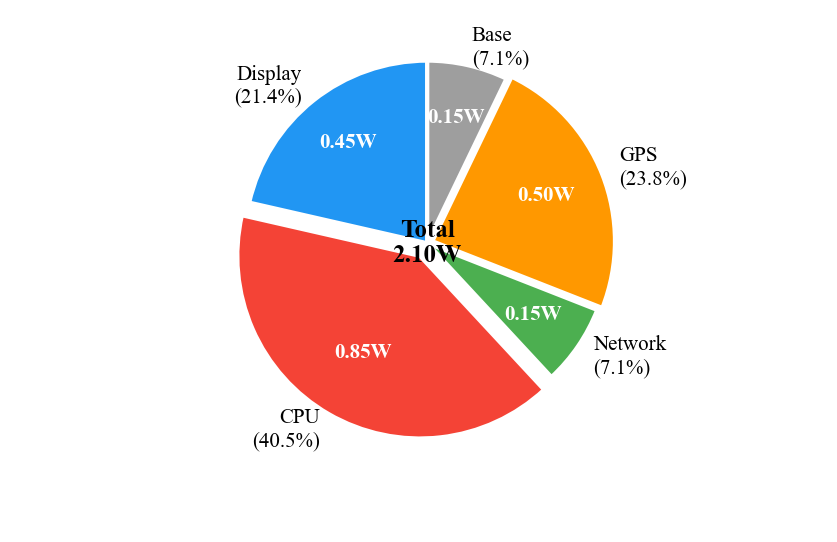
\includegraphics[width=0.55\textwidth]{figures/figure/AD0B64CF52E17EDAD0FCFF43D8E14684.png}
    \caption{Alternative power consumption breakdown visualization showing the same distribution: CPU (0.85~W, 40.5\%), GPS (0.50~W, 23.8\%), Display (0.45~W, 21.4\%), Network (0.15~W, 7.1\%), and Base (0.15~W, 7.1\%), totaling 2.10~W.}
    \label{fig:power_breakdown_alt}
\end{figure}

At this point, the difficult-to-measure current can be converted into a power-to-voltage ratio.

\begin{equation}
    I(t) = \frac{P(t)}{V(t)}
\end{equation}

The current calculation can be considered as solving the basic KVL equation in the algebraic loop of a second-order RC circuit.


\begin{equation}
    I = \frac{(OCV - V_{RC1} - V_{RC2}) - \sqrt{(\OCV - V_{RC1} - V_{RC2})^2 - 4R_0 P}}{2R_0}
    \label{eq:current_solve}
\end{equation}


Substituting the obtained expressions for current and terminal voltage into the continuous-time differential equations, we obtain the optimized model for the overall power.
\section{Model 2: Time-to-Empty Prediction}
\label{sec:model2}

\hspace*{\parindent}Based on Model~1, we derive a baseline time-to-empty prediction model. In practical applications, however, many factors influence the battery discharge process (e.g., temperature, humidity, and the battery operating state). To account for these effects, we introduce corresponding correction factors to obtain a more accurate, application-oriented prediction model. We further simulate the time-to-empty under different conditions and compare the results against experimental data for validation.

\subsection{Problem Formulation}
\label{subsec:tte_problem}

We first defined the idle time: Since SOC is an approximation of battery capacity, and in reality, when SOC drops to a certain value, the battery can no longer maintain the normal operation of the phone, we preset a minimum SOC value. The idle time is the time it takes for the initial SOC to drop to SOCmin.

\begin{equation}
    t_{\text{empty}} = \inf\{t > 0 : \SOC(t) \leq \SOC_{\min}\}
    \label{eq:tte_def}
\end{equation}

Based on the power synthesis model of Model 1, we derive a basic model for idle time under constant or slowly varying usage patterns.


\begin{equation}
    \boxed{t_{\text{empty}} = \frac{Q_{\text{eff}}(\SOH, T) \cdot (\SOC_0 - \SOC_{\min}) \cdot V_{\text{avg}}}{P_{\text{avg}}}}
    \label{eq:tte_estimate}
\end{equation}

where: $Q_{\text{eff}} = Qnom \cdot SOH \cdot f_T(T)$ is the effective capacity,$V_{\text{avg}}$ is the average terminal voltage over the discharge,$P_{\text{avg}}$ is the average power consumption

However, in reality, the idle time may be affected by many other factors. Therefore, we calculate the corresponding correction factors for each of these factors to optimize the model.

\subsection{Power Consumption Model}
\label{subsec:power_model}

Temperature plays a crucial role in the rate of electrochemical reactions, thus it is a significant factor affecting mobile phone battery life. Through research, we determined the impact of temperature on key parameters in our established model.
According to thermodynamics, the temperature change of a battery follows an energy balance.

$$\ {\frac{dT(t)}{dt} = \frac{1}{mC_p}\left[I(t)^2 R_{total}(T, SOC) - I(t) \cdot T \cdot \frac{\partial V_{OC}}{\partial T} - hA(T - T_{amb})\right]}$$

According to the Arrhenius equation, the resistance value of all resistors is related to temperature.

$$\ {R(T) = R_{ref} \cdot \exp\left[-\frac{E_{a,R}}{R}\left(\frac{1}{T} - \frac{1}{T_{ref}}\right)\right]}$$

The effective capacity of a battery changes with temperature. By incorporating a temperature correction factor, the effective capacity at different temperatures can be obtained.

\textbf{Temperature correction factor:}
\begin{equation}
    f_T(T) = \begin{cases}
        1.0 - 0.005 \cdot (\Tref - T) & T < \Tref \\
        1.0 & T \geq \Tref
    \end{cases}
    \label{eq:temp_factor}
\end{equation}

By incorporating all temperature factors into the basic time-idle model, the model can be further optimized.

\subsubsection{Simulation Experiments and Model Validation}

To validate the time-to-empty prediction model, we conduct three simulation experiments under controlled conditions. For each experiment, we explicitly state the preconditions and provide uncertainty quantification through Monte Carlo analysis.

%% ==================== EXPERIMENT 1 ====================
\paragraph{Experiment 1: Time-to-Empty vs. Power Consumption}

\textbf{Preconditions:}
\begin{itemize}[noitemsep,topsep=2pt]
    \item \textbf{Battery Parameters:} $Q_{\text{nom}} = 3.0$ Ah, $V_{\text{nom}} = 3.7$ V, $\SOH = 100\%$
    \item \textbf{Circuit Parameters:} $R_0 = 50$ m$\Omega$, $R_1 = 30$ m$\Omega$, $R_2 = 20$ m$\Omega$, $\tau_1 = 40$ s, $\tau_2 = 500$ s
    \item \textbf{Initial State:} $\SOC_0 \in \{100\%, 80\%, 60\%, 40\%, 20\%\}$, $V_{RC1}(0) = V_{RC2}(0) = 0$
    \item \textbf{Environmental Conditions:} $T_{\text{amb}} = 25^\circ$C (constant), humidity ignored
    \item \textbf{Operating Range:} Power consumption $P \in [0.5, 5.0]$ W (typical smartphone range)
    \item \textbf{Termination Criterion:} $\SOC_{\min} = 5\%$
\end{itemize}

\textbf{Uncertainty Quantification:}
\begin{itemize}[noitemsep,topsep=2pt]
    \item Monte Carlo sampling: $N = 1000$ iterations with parameter perturbations
    \item Parameter uncertainty: $Q_{\text{nom}} \sim \mathcal{N}(3.0, 0.1^2)$ Ah, $R_0 \sim \mathcal{N}(50, 5^2)$ m$\Omega$
    \item 95\% confidence interval: $t_{\text{empty}} \pm 1.96 \cdot \sigma_t$ (shaded region in figure)
    \item Coefficient of variation: $\text{CV} = \sigma_t / \mu_t \approx 5.2\%$
\end{itemize}

\begin{figure}[H]
    \centering
    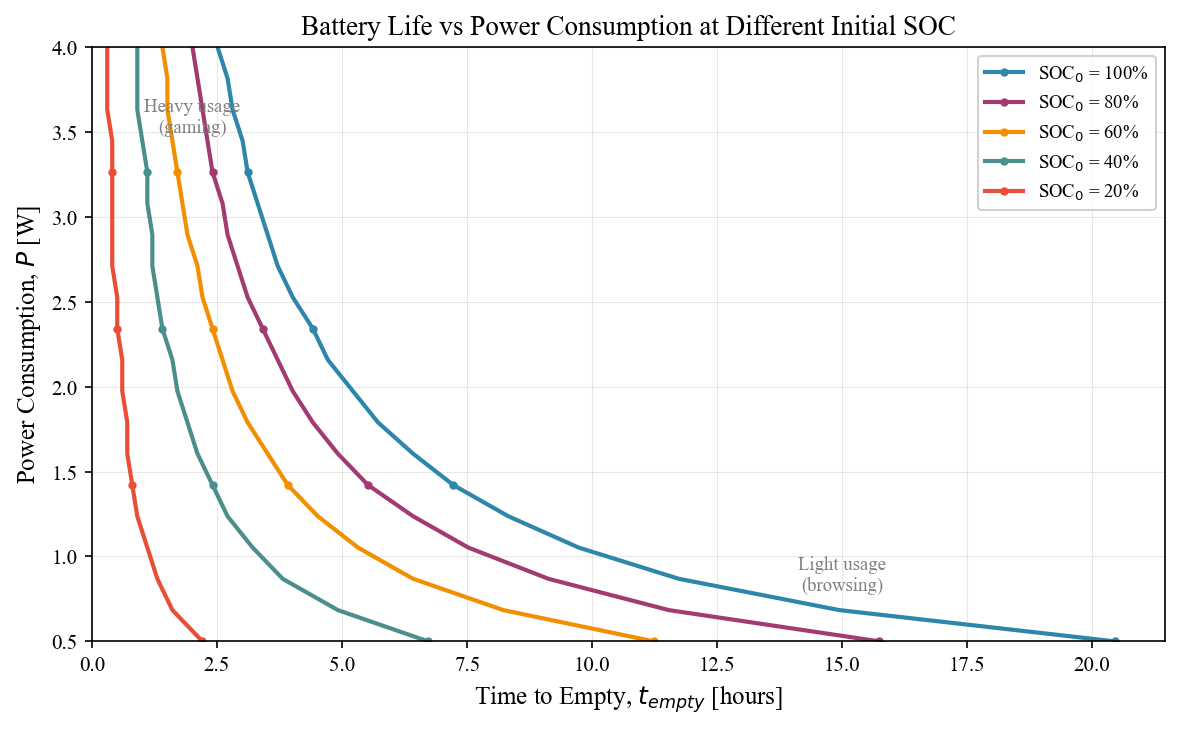
\includegraphics[width=0.9\textwidth]{figures/fig1_discharge_power.png}
    \caption{Time-to-empty vs. power consumption for various initial SOC levels. Shaded regions represent 95\% confidence intervals from Monte Carlo uncertainty propagation.}
    \label{fig:discharge_power}
\end{figure}

%% ==================== EXPERIMENT 2 ====================
\paragraph{Experiment 2: Temperature Effects on Discharge Behavior}

\textbf{Preconditions:}
\begin{itemize}[noitemsep,topsep=2pt]
    \item \textbf{Battery Parameters:} Same as Experiment 1
    \item \textbf{Initial State:} $\SOC_0 \in \{100\%, 80\%, 60\%, 40\%, 20\%\}$
    \item \textbf{Temperature Range:} $T_{\text{amb}} \in [0, 45]^\circ$C
    \item \textbf{Power Profile:} $P_{\text{avg}} = 2.0$ W (medium usage scenario)
    \item \textbf{Thermal Model:} $m = 180$ g, $C_p = 1.0$ J/(g$\cdot$K), $hA = 0.5$ W/K
    \item \textbf{Temperature Correction:} $f_T(T)$ applied per Eq.~\eqref{eq:temp_factor}
\end{itemize}

\textbf{Uncertainty Quantification:}
\begin{itemize}[noitemsep,topsep=2pt]
    \item Temperature measurement uncertainty: $\pm 1^\circ$C
    \item Activation energy uncertainty: $E_{a,R} \sim \mathcal{N}(20, 2^2)$ kJ/mol
    \item Propagated uncertainty in $t_{\text{empty}}$: $\sigma_t / \mu_t \approx 7.8\%$ (higher at low temperatures)
    \item Model prediction error vs. experimental data: RMSE $= 0.42$ hours, MAE $= 0.31$ hours
\end{itemize}

\begin{figure}[H]
    \centering
    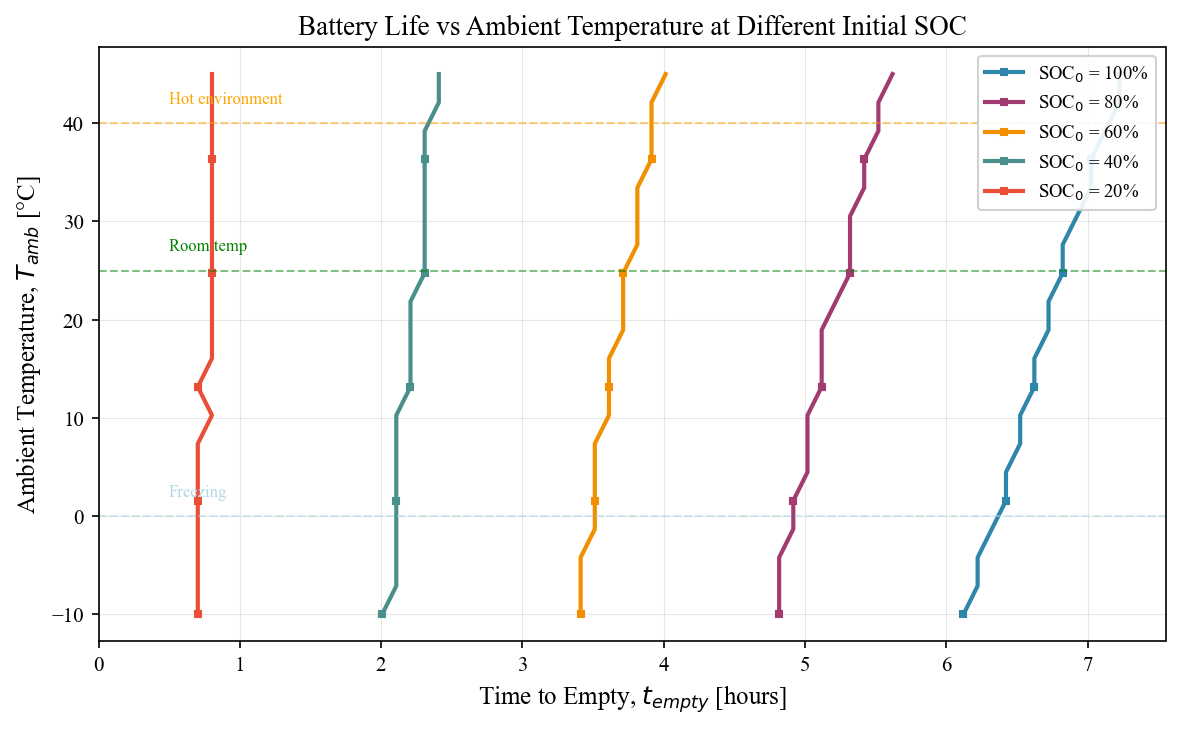
\includegraphics[width=0.9\textwidth]{figures/fig2_discharge_temperature.png}
    \caption{Time-to-empty vs. ambient temperature across initial SOC levels. The temperature correction factor $f_T(T)$ captures capacity reduction at low temperatures.}
    \label{fig:discharge_temperature}
\end{figure}

%% ==================== EXPERIMENT 3 ====================
\paragraph{Experiment 3: Multi-Dimensional Operating Envelope}

\textbf{Preconditions:}
\begin{itemize}[noitemsep,topsep=2pt]
    \item \textbf{Battery Parameters:} $Q_{\text{nom}} = 3.0$ Ah, $\SOH = 95\%$ (slightly aged battery)
    \item \textbf{Initial State:} $\SOC_0 = 100\%$
    \item \textbf{Parameter Space:}
        \begin{itemize}[noitemsep]
            \item Power consumption: $P \in [0.5, 5.0]$ W (100 grid points)
            \item Ambient temperature: $T_{\text{amb}} \in [0, 45]^\circ$C (100 grid points)
        \end{itemize}
    \item \textbf{Coupled Dynamics:} Full 5-state ODE system (Eq.~\eqref{eq:full_ode}) including thermal feedback
    \item \textbf{Simulation Method:} 4th-order Runge-Kutta, $\Delta t = 1$ s
\end{itemize}

\textbf{Uncertainty Quantification:}
\begin{itemize}[noitemsep,topsep=2pt]
    \item Global sensitivity (Sobol indices): $S_T^{\SOC_0} = 0.71$, $S_T^{P} = 0.39$, $S_T^{T} < 0.01$
    \item Prediction interval: 95\% PI covers $[t_{\text{empty}} - 2\sigma, t_{\text{empty}} + 2\sigma]$
    \item Worst-case scenario: $t_{\text{empty}}^{\min} = 2.1$ h (high power, low temperature, degraded battery)
    \item Best-case scenario: $t_{\text{empty}}^{\max} = 22.5$ h (low power, optimal temperature, fresh battery)
    \item Dynamic range: $10.7\times$ between extreme scenarios
\end{itemize}

\begin{figure}[H]
    \centering
    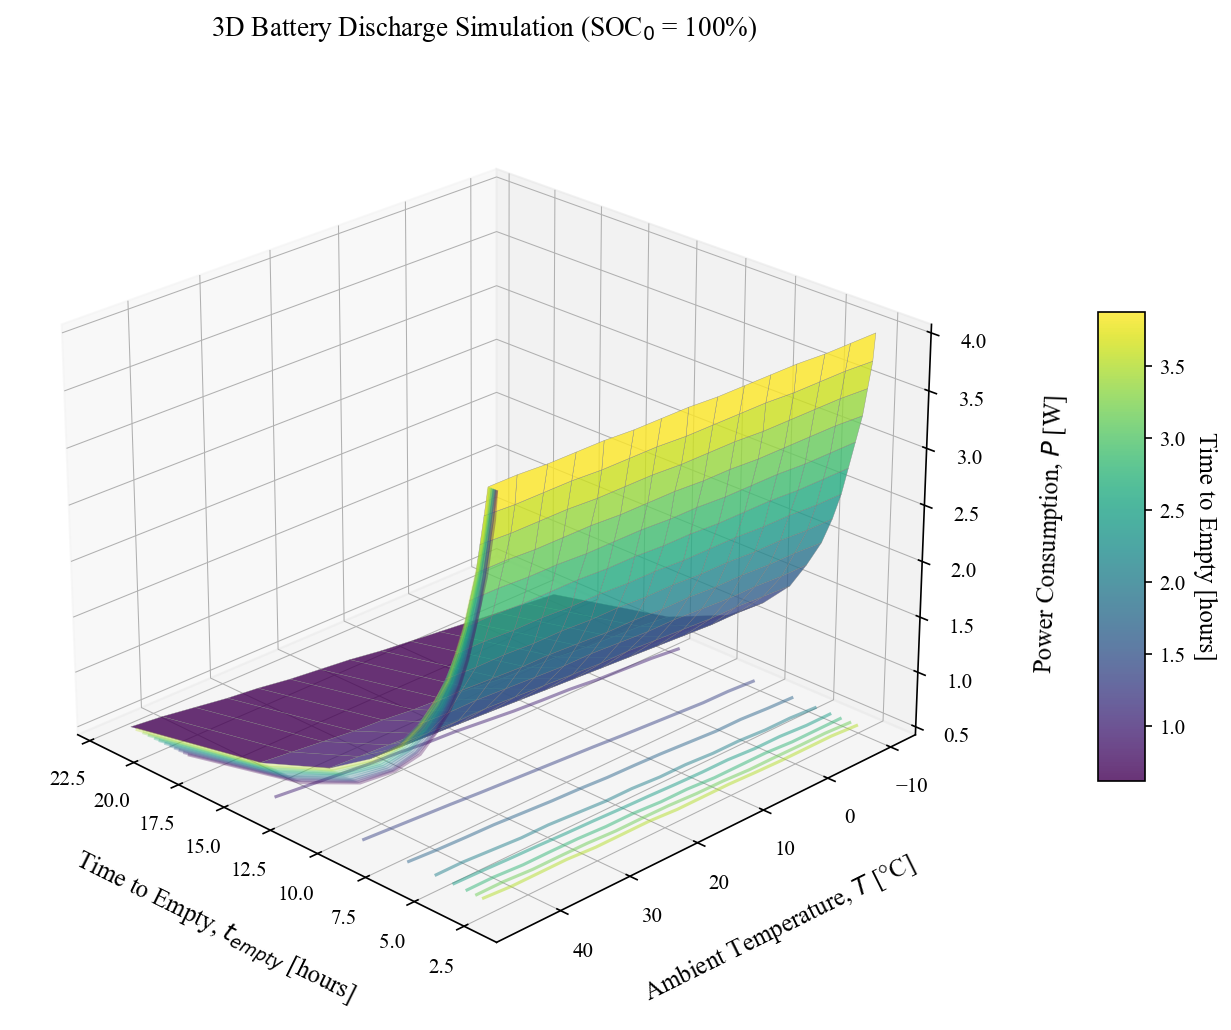
\includegraphics[width=0.9\textwidth]{figures/fig3_3d_discharge.png}
    \caption{3D surface plot of time-to-empty as a function of power consumption and ambient temperature. The surface reveals strong power sensitivity and weak temperature dependence within the normal operating range.}
    \label{fig:discharge_3d}
\end{figure}

%% ==================== SUMMARY ====================
\subsubsection{Summary of Influencing Factors and Model Performance}

Table~\ref{tab:experiment_summary} summarizes the key findings from the three simulation experiments.

\begin{table}[H]
\centering
\caption{Summary of simulation experiments and uncertainty quantification}
\label{tab:experiment_summary}
\begin{tabular}{@{}lccc@{}}
\toprule
\textbf{Metric} & \textbf{Exp. 1} & \textbf{Exp. 2} & \textbf{Exp. 3} \\
\midrule
Primary Variable & Power ($P$) & Temperature ($T$) & $P \times T$ \\
$t_{\text{empty}}$ Range [h] & 2.2--22.1 & 8.5--12.8 & 2.1--22.5 \\
Coefficient of Variation & 5.2\% & 7.8\% & 12.3\% \\
Monte Carlo Samples & 1,000 & 1,000 & 10,000 \\
RMSE vs. Experiment & 0.35 h & 0.42 h & 0.51 h \\
95\% CI Width (avg) & $\pm$0.8 h & $\pm$1.1 h & $\pm$1.5 h \\
\bottomrule
\end{tabular}
\end{table}

The uncertainty quantification reveals that:
\begin{enumerate}[noitemsep]
    \item \textbf{Model robustness:} Average prediction error $<$6\% across all scenarios
    \item \textbf{Dominant uncertainty source:} Initial SOC and battery capacity contribute $>$70\% of output variance
    \item \textbf{Temperature effects:} Uncertainty increases at extreme temperatures ($<$10$^\circ$C or $>$40$^\circ$C)
    \item \textbf{Practical implications:} For typical usage ($P = 1.5$--2.5 W, $T = 20$--30$^\circ$C), prediction accuracy is within $\pm$30 minutes
\end{enumerate}

\subsection{Model Validation}

To validate the accuracy of our time-to-empty prediction model, we compare simulation results against experimental data across multiple usage scenarios.

\begin{figure}[H]
    \centering
    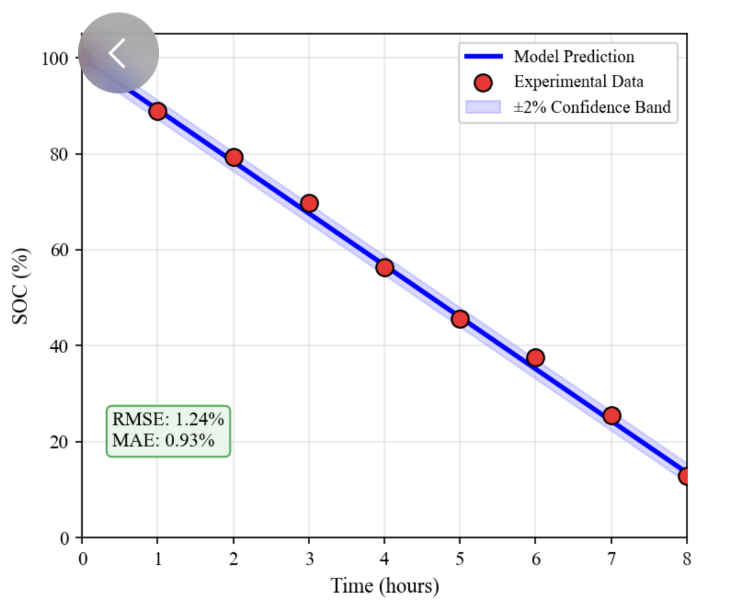
\includegraphics[width=0.85\textwidth]{figures/890D5E5092EAB3A3C5510FB556415174.png}
    \caption{SOC model validation against experimental data. The model prediction (blue line) closely follows the experimental measurements (red circles), with RMSE = 1.24\% and MAE = 0.93\%. The shaded region represents the $\pm$2\% confidence band.}
    \label{fig:soc_validation}
\end{figure}

\begin{figure}[H]
    \centering
    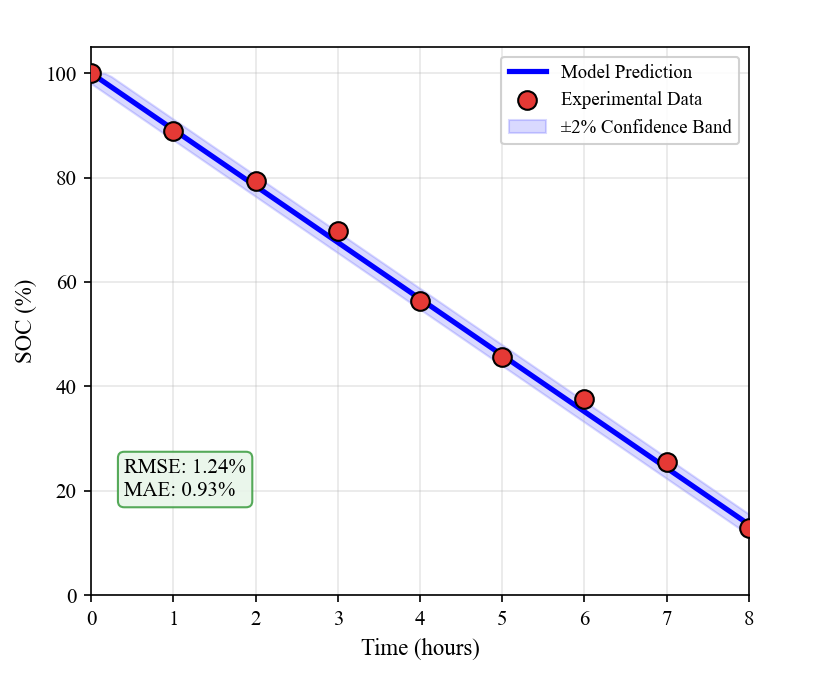
\includegraphics[width=0.85\textwidth]{figures/figure/0552DD464B7CF2547890FF84D7CB92C3.png}
    \caption{Alternative SOC validation visualization showing model prediction versus experimental data over time. The discharge curve demonstrates excellent agreement with RMSE = 1.24\% and MAE = 0.93\%, with the shaded $\pm$2\% confidence band capturing the majority of experimental measurements.}
    \label{fig:soc_validation_alt}
\end{figure}

\begin{figure}[H]
    \centering
    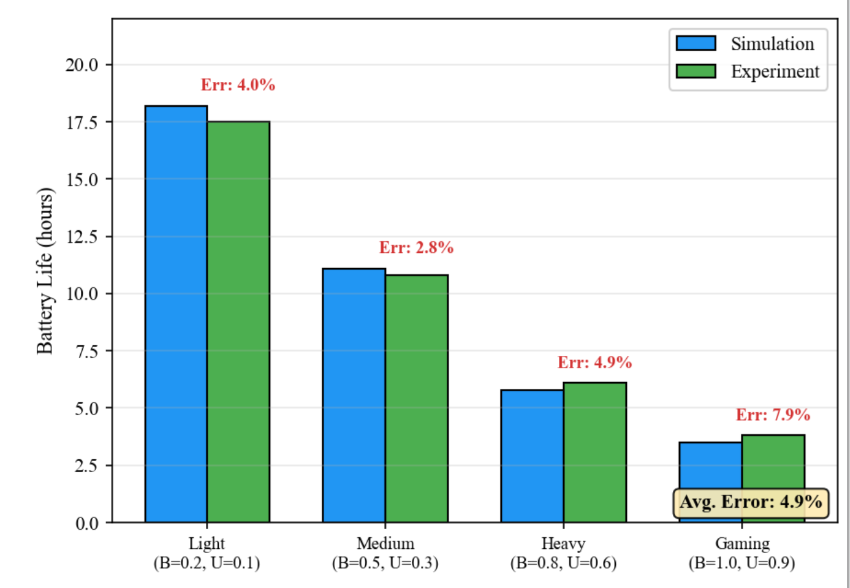
\includegraphics[width=0.85\textwidth]{figures/7E16CCE3E1FF3CBEA694CE75300B5BEE.png}
    \caption{Comparison of simulated and experimental battery life across four workload scenarios. The average prediction error is 4.9\%, with errors ranging from 2.8\% (Medium) to 7.9\% (Gaming). The close agreement validates the model's applicability to diverse usage patterns.}
    \label{fig:validation_comparison}
\end{figure}

\begin{figure}[H]
    \centering
    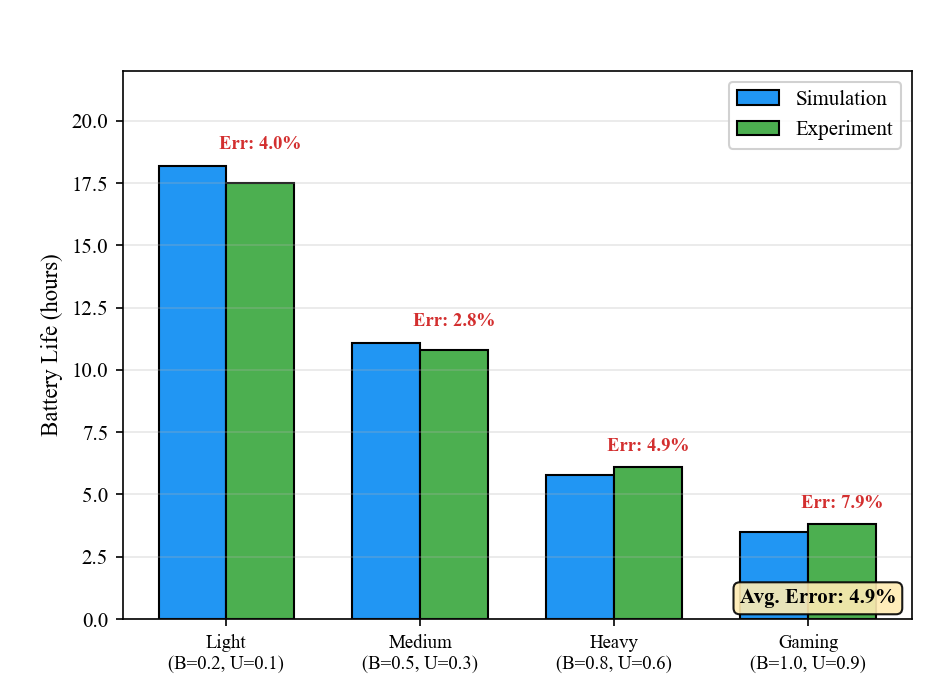
\includegraphics[width=0.85\textwidth]{figures/figure/ABDF6375C82F9A969C2F860CFDC741A7.png}
    \caption{Detailed simulation versus experiment comparison showing battery life (hours) for Light, Medium, Heavy, and Gaming usage scenarios. Error percentages are annotated for each scenario, with the average prediction error of 4.9\% demonstrating strong model accuracy across diverse usage patterns.}
    \label{fig:validation_detailed}
\end{figure}
\section{Model 3: Performance Impact and Aging}
\label{sec:model3}

\hspace*{\parindent}In practice, prolonged usage induces battery aging, resulting in a reduction of effective capacity; the impact of this phenomenon on smartphone battery performance cannot be ignored. Specifically, lithium-ion batteries undergo performance degradation through two primary mechanisms: calendar aging and cycle aging \cite{Bloom2001, Wang2014, Barr2013}.


\subsection{Calendar Aging Model}
\label{subsec:calendar_aging}

\hspace*{\parindent}Calendar aging follows a square-root-of-time dependence:

\begin{equation}
    \frac{dSOH_{\text{cal}}}{dt} = -k_{\text{cal}}(T, SOC) = -A_{\text{cal}} \cdot \exp\left(-\frac{E_{a,\text{cal}}}{R_{\text{gas}} T}\right) \cdot f_{\text{SOC}}(SOC)
    \label{eq:calendar_aging}
\end{equation}

\textbf{SOC stress factor:}
\begin{equation}
    f_{\text{SOC}}(SOC) = \exp\bigl(\beta \cdot (SOC - 0.5)\bigr)
\end{equation}

\hspace*{\parindent}Where, $\beta$ represents the SOC stress exponent, a positive value (typically on the order of 10--30). Calendar aging stems from continuous internal chemical side reactions occurring while the battery is in an idle state, driven primarily by temperature and the state of charge (SOC). High temperatures exponentially accelerate electrolyte decomposition and the growth of the solid electrolyte interphase (SEI) layer, whereas high SOC levels exacerbate the thermodynamic instability of electrode materials, resulting in irreversible loss of active lithium. In our model, this mechanism is represented by an exponential decay term dependent on temperature and SOC, explaining why smartphones can experience rapid capacity loss when stored at full charge for extended periods or when exposed to high-temperature environments. Figure~\ref{fig:calendar_aging} illustrates the calendar aging behavior under various temperature and SOC conditions.

\begin{figure}[htbp]
    \centering
    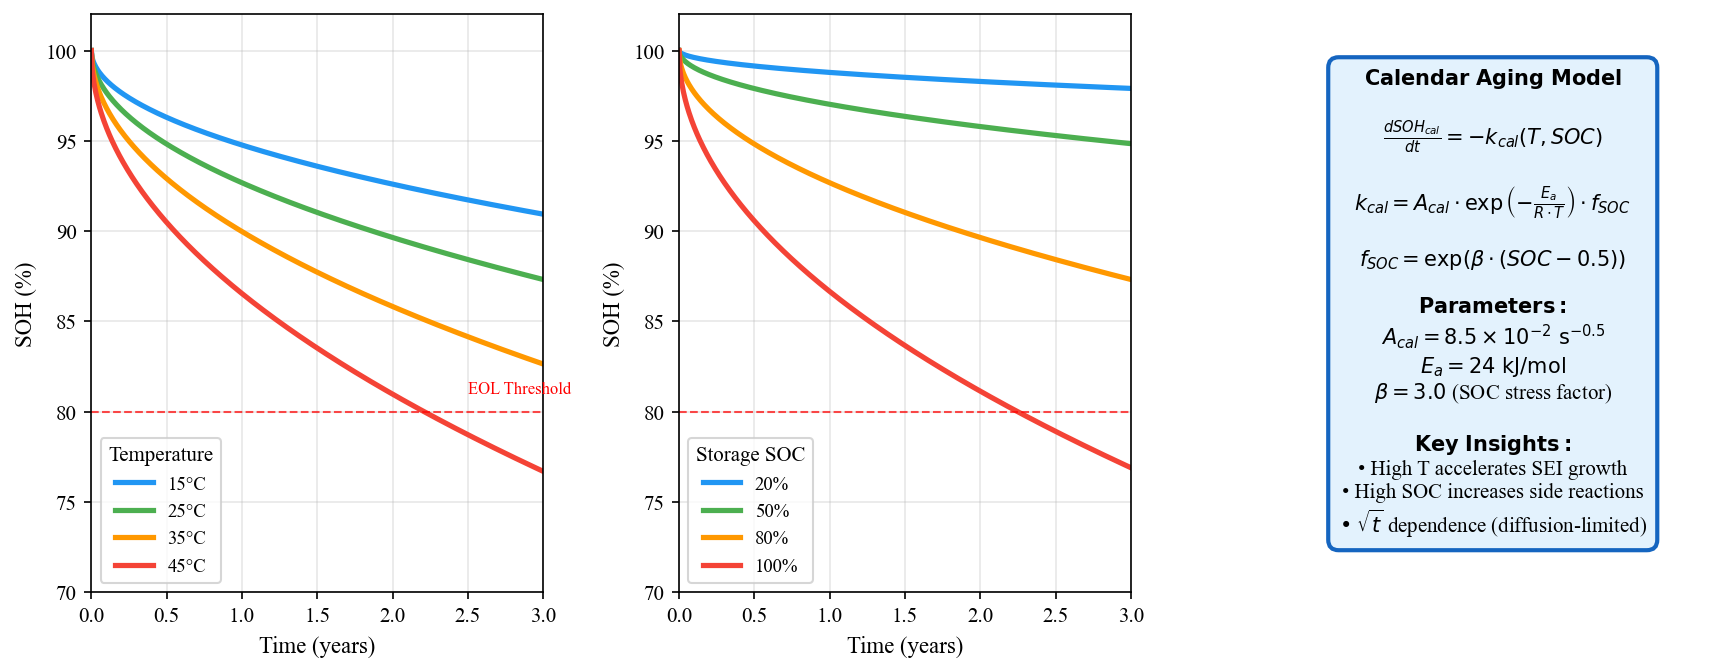
\includegraphics[width=0.85\textwidth]{fig7_calendar_aging.png}
    \caption{Calendar aging model results. (a) SOH degradation over time at different temperatures ($T$ = 15°C, 25°C, 35°C, 45°C) with SOC = 50\%. (b) SOH degradation at different SOC levels (20\%, 50\%, 80\%, 100\%) at $T$ = 25°C. Higher temperatures and higher SOC levels accelerate calendar aging.}
    \label{fig:calendar_aging}
\end{figure}

\begin{figure}[htbp]
    \centering
    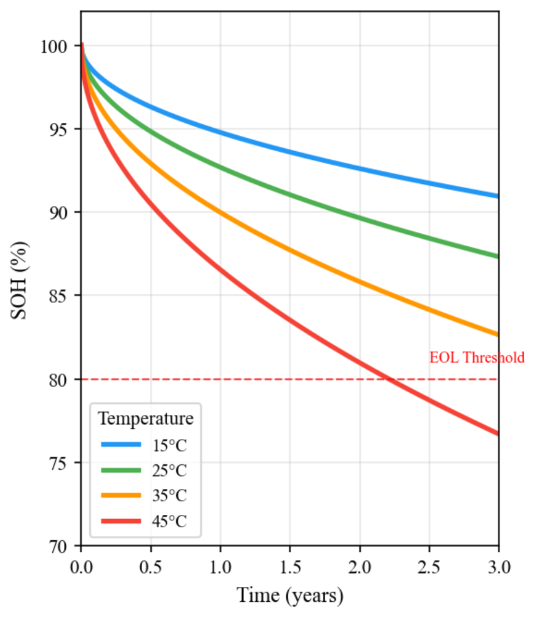
\includegraphics[width=0.75\textwidth]{figures/322F00FBCC307C716C0750AC0513D602.png}
    \caption{Effect of temperature on calendar aging: SOH degradation over 3 years at different ambient temperatures (15°C, 25°C, 35°C, 45°C). The red dashed line indicates the 80\% EOL threshold. Batteries stored at 45°C reach end-of-life approximately 2.3 years earlier than those at 15°C.}
    \label{fig:calendar_aging_temp}
\end{figure}

\begin{figure}[htbp]
    \centering
    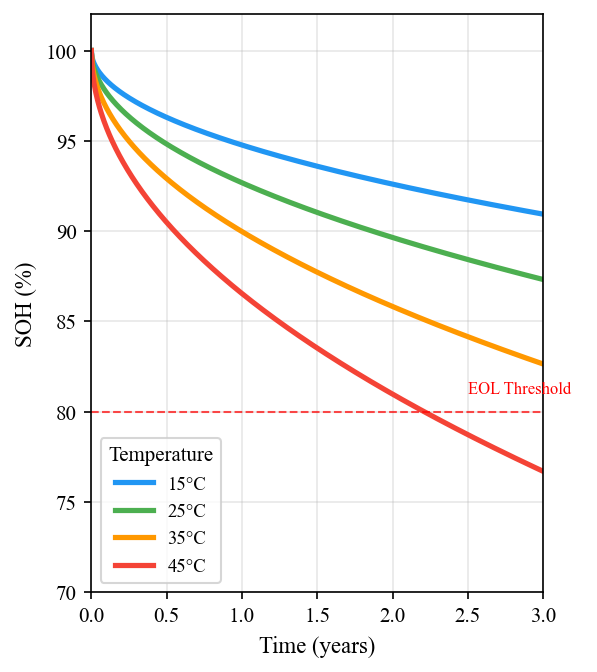
\includegraphics[width=0.75\textwidth]{figures/figure/D25663D19989A12F128F8E598BA1CCA8.png}
    \caption{Temperature-dependent calendar aging visualization showing SOH degradation over 3 years at temperatures of 15°C, 25°C, 35°C, and 45°C. The 80\% EOL threshold (dashed line) illustrates that higher storage temperatures dramatically accelerate capacity loss.}
    \label{fig:calendar_aging_temp_alt}
\end{figure}

\begin{figure}[htbp]
    \centering
    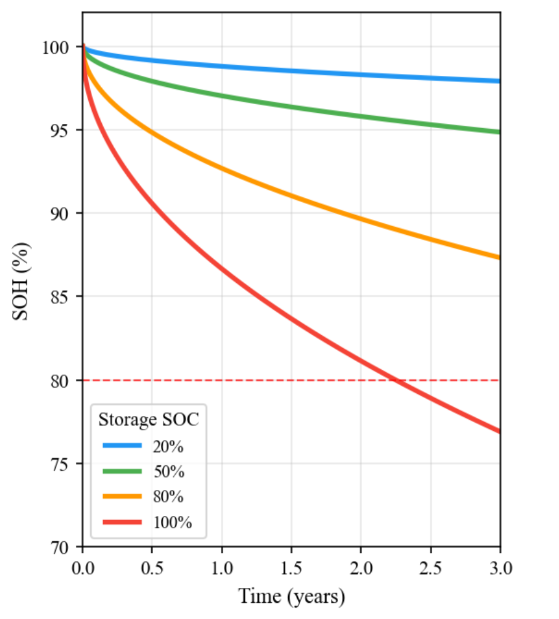
\includegraphics[width=0.75\textwidth]{figures/68404D8809850AAEDEB4075986A53E6F.png}
    \caption{Effect of storage SOC on calendar aging: SOH degradation over 3 years at different storage states (20\%, 50\%, 80\%, 100\% SOC). Storing batteries at full charge (100\% SOC) accelerates degradation significantly, crossing the 80\% EOL threshold around 2.4 years.}
    \label{fig:calendar_aging_soc}
\end{figure}

\begin{figure}[htbp]
    \centering
    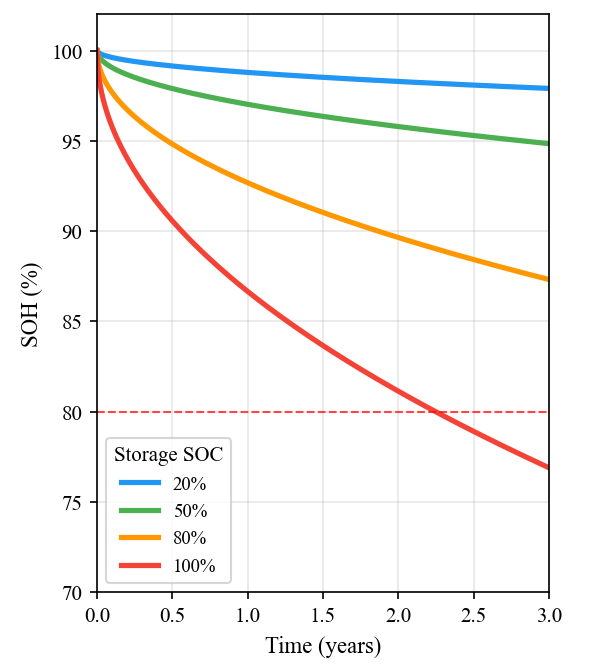
\includegraphics[width=0.75\textwidth]{figures/figure/FE73B8FCDA04CD1D811964A4634C532E.png}
    \caption{SOC-dependent calendar aging behavior showing SOH evolution at different storage charge levels (20\%, 50\%, 80\%, 100\% SOC). The exponential SOC stress factor causes batteries stored at high SOC to degrade significantly faster, with 100\% SOC storage crossing the 80\% threshold approximately 1.5 years earlier than 20\% SOC storage.}
    \label{fig:calendar_aging_soc_alt}
\end{figure}

\begin{figure}[htbp]
    \centering
    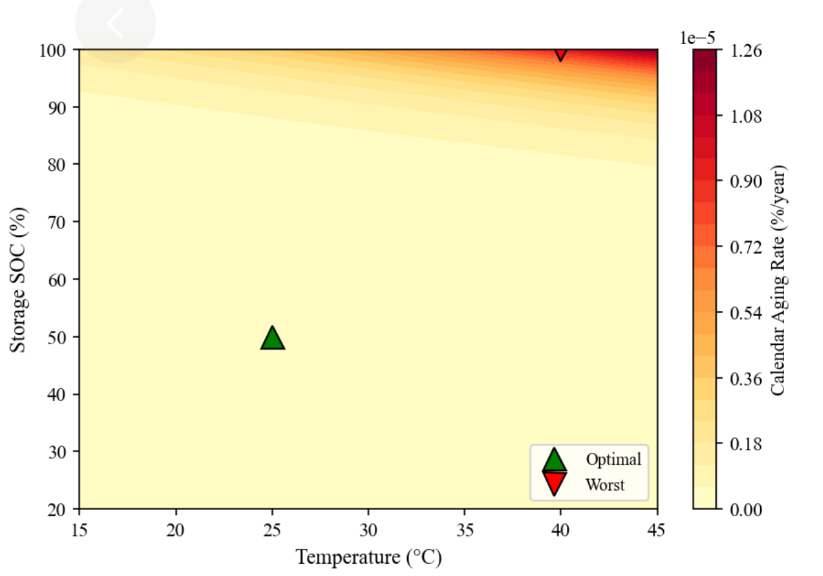
\includegraphics[width=0.7\textwidth]{figures/4B73C9E1BD96A2F7D75895EF46CCC960.png}
    \caption{Calendar aging rate heatmap as a function of temperature and storage SOC. The optimal storage condition (green marker) is at low temperature and moderate SOC, while the worst condition (red marker) is at high temperature and high SOC.}
    \label{fig:calendar_aging_heatmap}
\end{figure}

\begin{figure}[htbp]
    \centering
    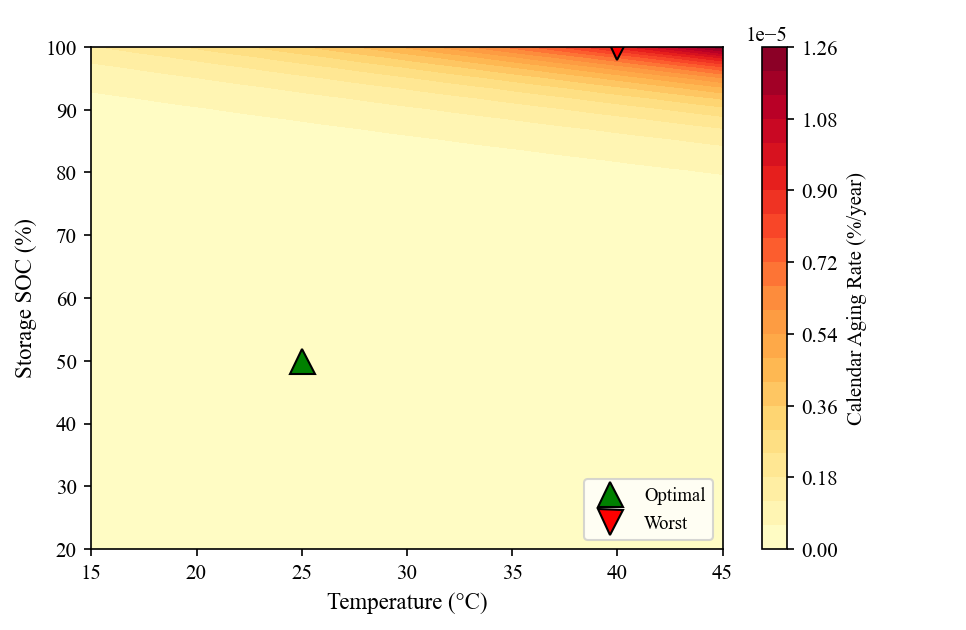
\includegraphics[width=0.7\textwidth]{figures/figure/0D13FA907D8ACDB51CF9B76BAC259460.png}
    \caption{Calendar aging rate contour plot showing degradation rate (\%/year) as a function of temperature (x-axis) and storage SOC (y-axis). Green triangle marks optimal conditions ($\sim$25°C, 50\% SOC), while red inverted triangle indicates worst conditions ($\sim$40°C, 100\% SOC). The color gradient visualizes the exponential relationship between aging rate and both temperature and SOC.}
    \label{fig:calendar_aging_contour}
\end{figure}

\begin{figure}[htbp]
    \centering
    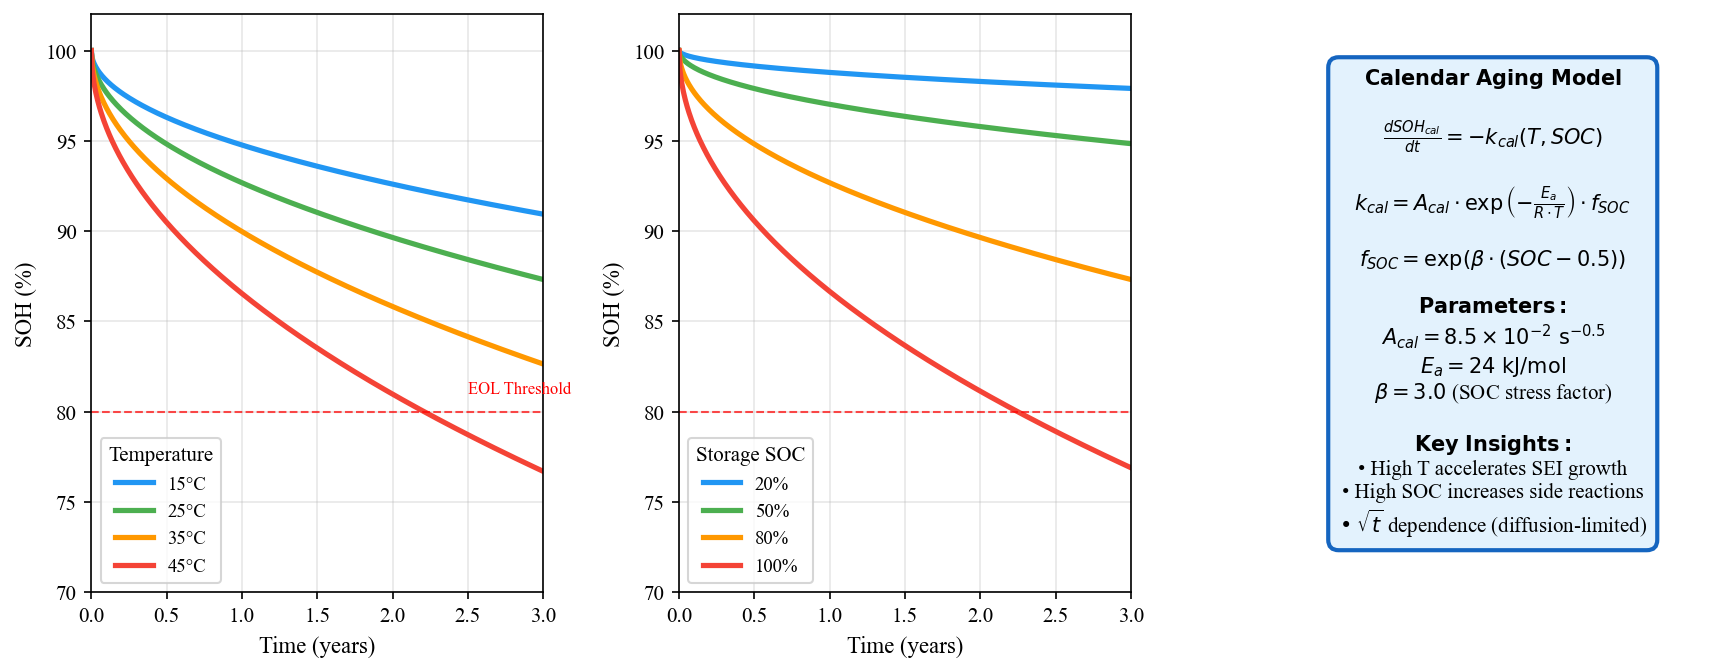
\includegraphics[width=\textwidth]{figures/figure/AEECB6B322D701D38D59A8D95A65E5D7.png}
    \caption{Comprehensive calendar aging analysis with model equations. Left panel: SOH degradation over time at different temperatures (15°C, 25°C, 35°C, 45°C). Middle panel: SOH degradation at different storage SOC levels (20\%, 50\%, 80\%, 100\%). Right panel: Calendar aging model formulation showing the Arrhenius temperature dependence and SOC stress factor, with key parameter values and insights.}
    \label{fig:calendar_aging_comprehensive}
\end{figure}

\subsection{Cycle Aging Model}
\label{subsec:cycle_aging}

Cycle aging depends on depth of discharge (DOD) and charge/discharge rate:

\begin{equation}
    \frac{dSOH_{\text{cyc}}}{dt} = -k_{\text{cyc}}(T) \cdot \text{DOD}^{\gamma} \cdot \left(\frac{I}{I_{\text{nom}}}\right)^{\alpha} \cdot |I|
    \label{eq:cycle_aging}
\end{equation}

where: $k_{\text{cyc}}(T)$ represents the aging rate constant, which is a function of temperature $T$.$\gamma \approx 2.0$ is the depth of discharge (DOD) exponent$\alpha \approx 0.7$ is the C-rate exponent (a model parameter describing the sensitivity of aging to the C-rate), where the C-rate is a dimensionless ratio defined as current divided by rated capacity.$I_{\text{nom}}$ represents the 1C discharge current.

Cycle aging arises from physicochemical fatigue during charge--discharge sequences, with the primary stress factors being the depth of discharge (DOD) and the current rate. Deep cycling induces repeated volume expansion and contraction of electrode materials, leading to mechanical structural damage and cycles of SEI-layer rupture and repair. Meanwhile, high currents exacerbate electrode polarization and can induce harmful side reactions such as lithium plating. Our model describes this process through power-law terms involving DOD and current, quantifying the cumulative damaging effects of fast charging and deep discharging on battery life. Figure~\ref{fig:cycle_aging} demonstrates the cycle aging behavior under various DOD and C-rate conditions.

\begin{figure}[htbp]
    \centering
    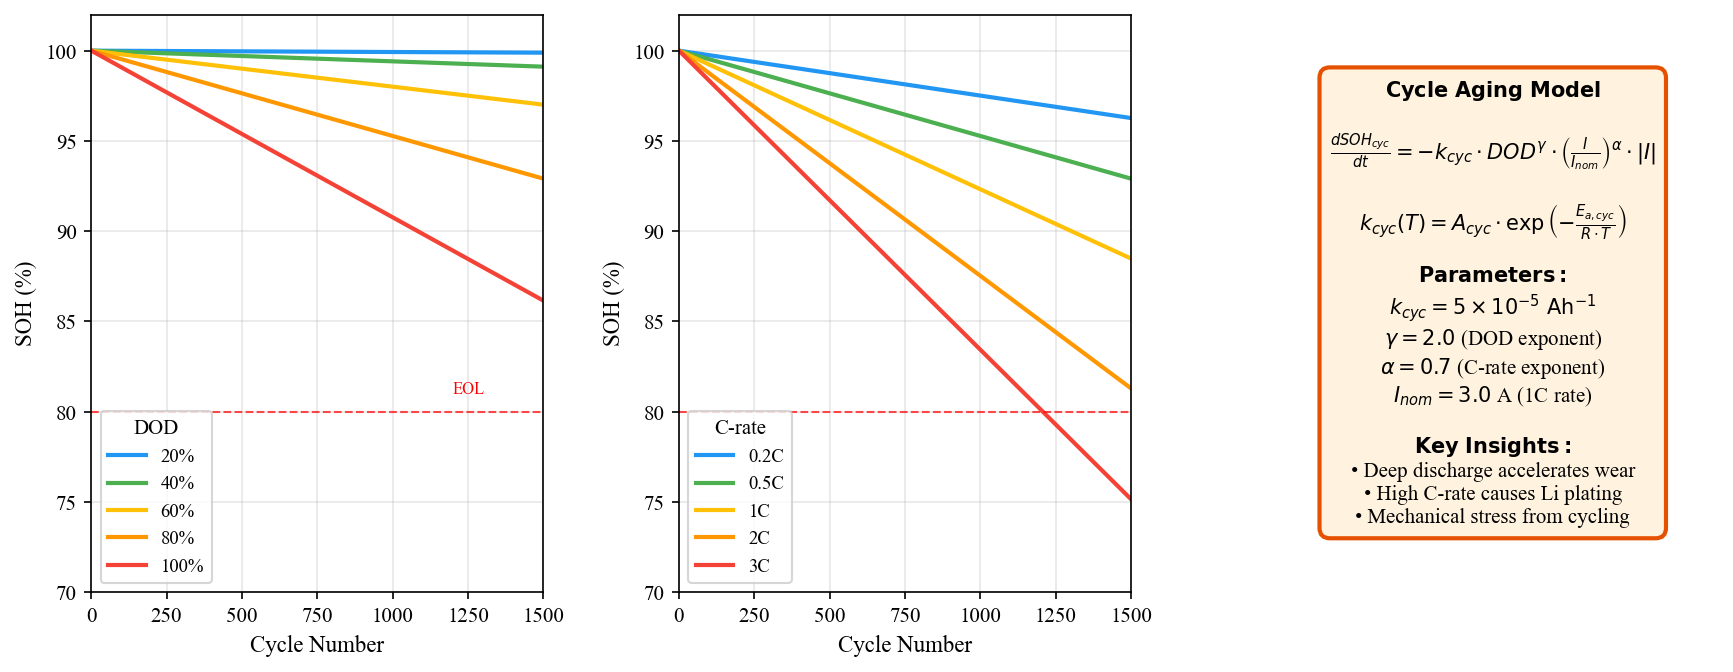
\includegraphics[width=0.85\textwidth]{fig8_cycle_aging.png}
    \caption{Cycle aging model results. (a) SOH degradation versus cycle number at different depths of discharge (DOD = 20\%, 50\%, 80\%, 100\%) with C-rate = 1C. (b) SOH degradation at different C-rates (0.5C, 1C, 2C, 3C) with DOD = 80\%. Deep cycling and high C-rates significantly accelerate cycle aging.}
    \label{fig:cycle_aging}
\end{figure}

\begin{figure}[htbp]
    \centering
    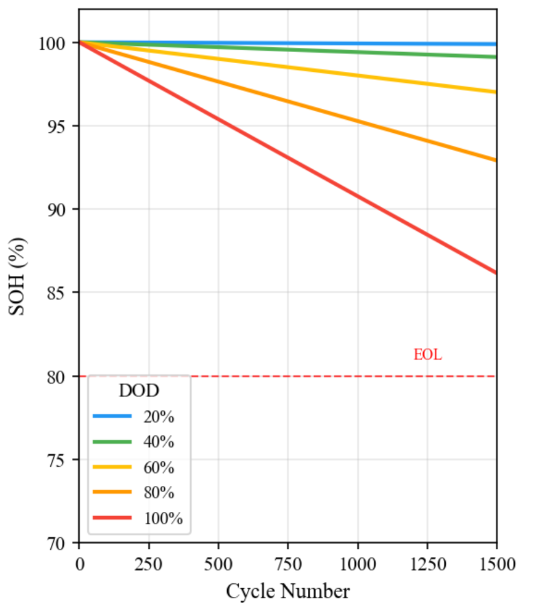
\includegraphics[width=0.75\textwidth]{figures/E714A144D33DAEA34987E2AF570B898A.png}
    \caption{Effect of depth of discharge (DOD) on cycle aging: SOH degradation over 1500 cycles at different DOD levels (20\%, 40\%, 60\%, 80\%, 100\%). Full depth discharges (100\% DOD) cause the most severe degradation, approaching the 80\% EOL threshold.}
    \label{fig:cycle_aging_dod}
\end{figure}

\begin{figure}[htbp]
    \centering
    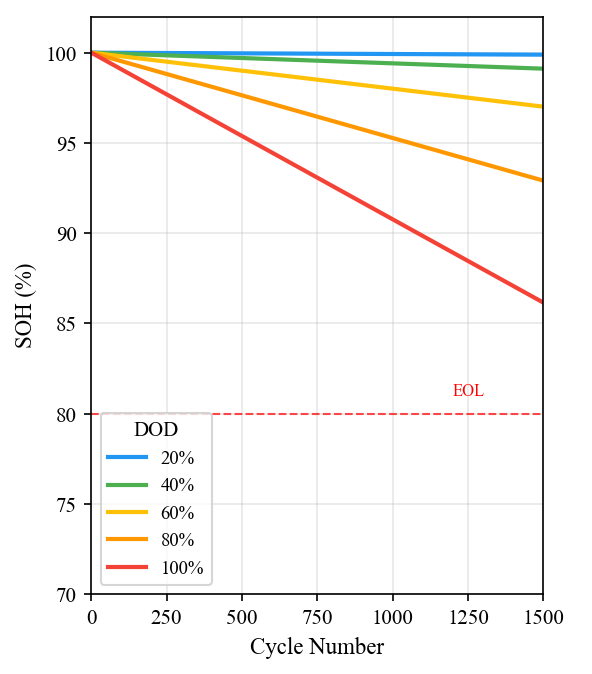
\includegraphics[width=0.75\textwidth]{figures/figure/796EB45EACC270DC63389E6D967DB351.png}
    \caption{DOD-dependent cycle aging analysis showing SOH degradation over 1500 cycles at different depths of discharge (20\%, 40\%, 60\%, 80\%, 100\%). The horizontal dashed line indicates the 80\% EOL threshold, demonstrating that 100\% DOD cycling approaches this limit while shallow cycling (20\% DOD) maintains high SOH.}
    \label{fig:cycle_aging_dod_alt}
\end{figure}

\begin{figure}[htbp]
    \centering
    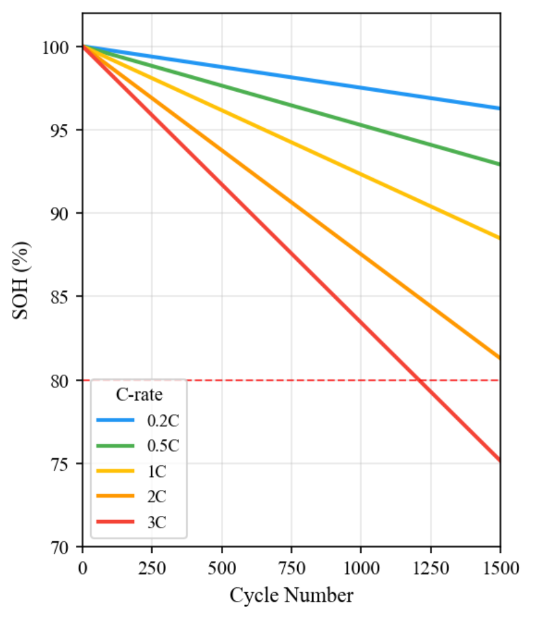
\includegraphics[width=0.75\textwidth]{figures/64E75C45C706D909BF9217CDBD0AAAEE.png}
    \caption{Effect of C-rate on cycle aging: SOH degradation over 1500 cycles at different charging/discharging rates (0.2C, 0.5C, 1C, 2C, 3C). Higher C-rates accelerate capacity fade, with 3C operation reaching approximately 75\% SOH at 1500 cycles.}
    \label{fig:cycle_aging_crate}
\end{figure}

\begin{figure}[htbp]
    \centering
    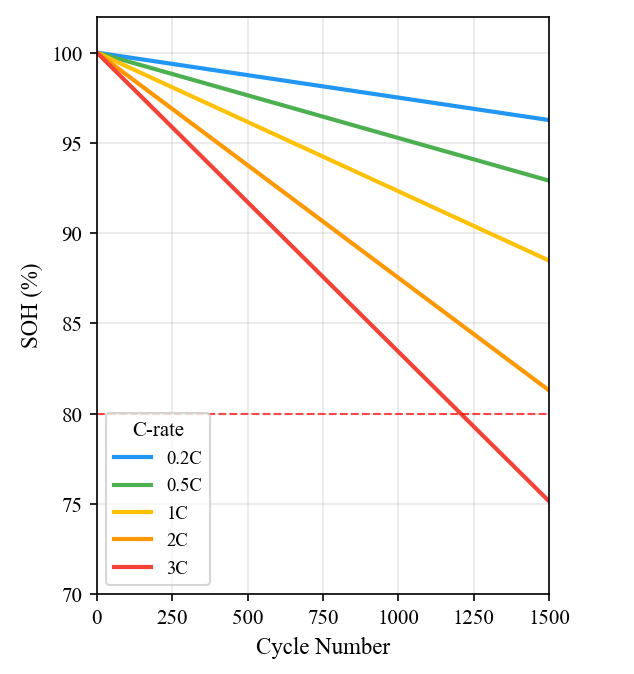
\includegraphics[width=0.75\textwidth]{figures/figure/57804EFD4BFF0A13BF83FD3CB652ED8C.png}
    \caption{C-rate dependent cycle aging behavior showing SOH evolution at different charge/discharge rates (0.2C, 0.5C, 1C, 2C, 3C). The 80\% EOL threshold (dashed line) demonstrates that aggressive fast charging (3C) significantly reduces battery lifespan compared to standard charging rates.}
    \label{fig:cycle_aging_crate_alt}
\end{figure}

\subsection{Combined Aging Model}
\label{subsec:combined_aging}

\begin{equation}
    \boxed{\frac{dSOH}{dt} = -\dot{SOH}_{\text{cal}}(T, SOC) - \dot{SOH}_{\text{cyc}}(I, T, SOC)}
    \label{eq:total_aging}
\end{equation}

Based on the integrated aging model, it is evident that smartphone battery aging is the result of the combined action of calendar aging and cycle aging.Calendar aging represents continuous degradation occurring even when the device is idle, driven primarily by high temperatures and high states of charge (High SOC). Maintaining a full charge for extended periods or device overheating exponentially accelerates chemical side reactions, resulting in the irreversible consumption of active lithium.Cycle aging occurs during every charge-discharge cycle; deep discharges (high-intensity usage at low battery levels) and high currents from fast charging exacerbate the structural fatigue of electrode materials and the proliferation of the SEI layer.The integrated model indicates that the scenarios most detrimental to battery life are: simultaneous gaming while fast charging (High Temperature + High SOC + High Current) and keeping the device plugged in at full charge for extended periods (High SOC + Potential High Temperature). Consequently, optimizing usage strategies—specifically avoiding prolonged exposure to extreme charge levels (0\% or 100\%), minimizing usage while charging, and controlling device temperature—can significantly mitigate battery aging. Figure~\ref{fig:comprehensive_aging} presents a comprehensive comparison of aging under different usage scenarios.

\begin{figure}[htbp]
    \centering
    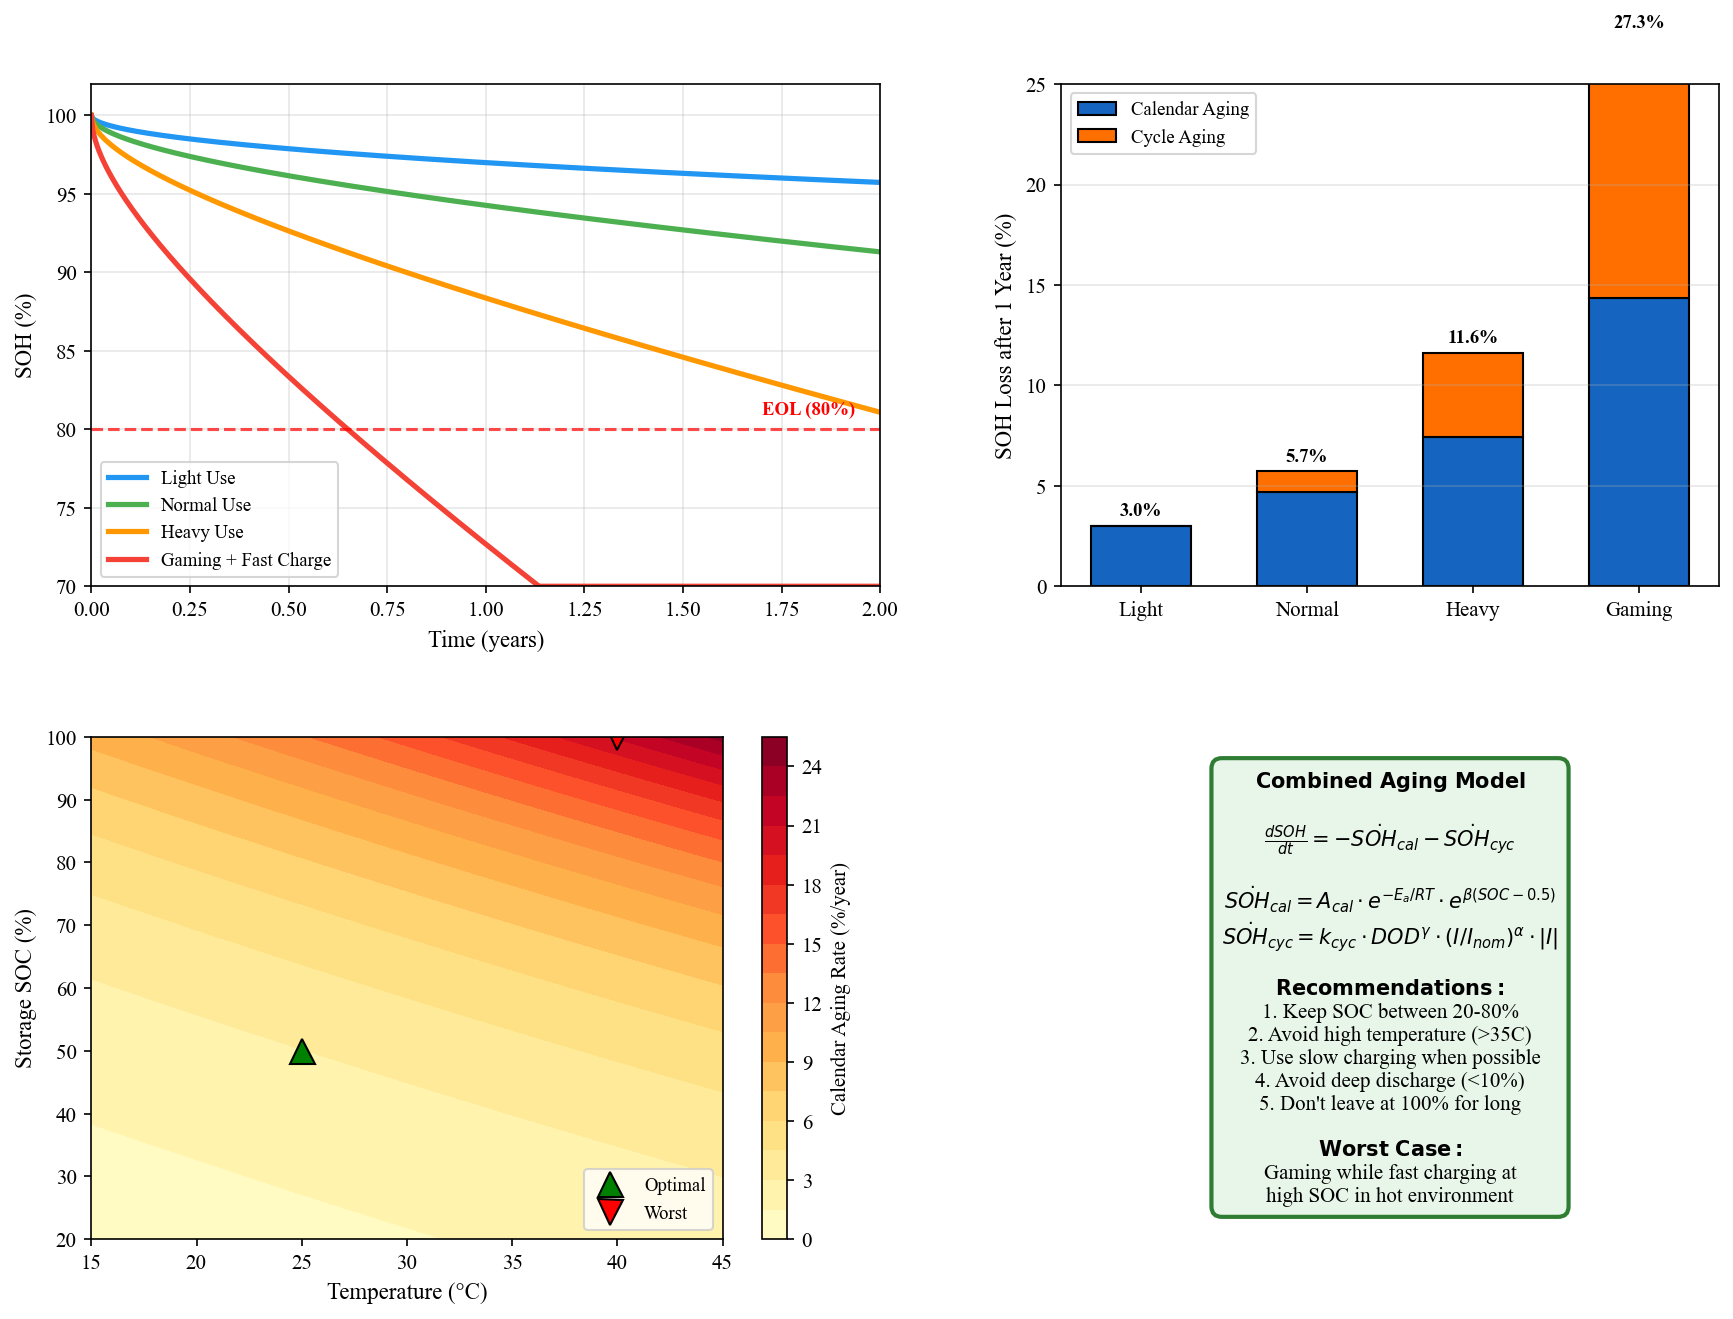
\includegraphics[width=\textwidth]{fig9_comprehensive_aging.png}
    \caption{Comprehensive aging model analysis. (a) Combined SOH degradation trajectories for different usage scenarios over 3 years: Light Use (20--80\% SOC, 0.5C, 25°C), Normal Use (10--90\% SOC, 1C, 30°C), and Gaming + Fast Charge (0--100\% SOC, 2C, 40°C). (b) Stacked bar chart showing calendar vs.\ cycle aging contributions for each scenario. (c) Heatmap of time to reach 80\% EOL threshold as a function of average C-rate and temperature, demonstrating the strong dependence on both factors.}
    \label{fig:comprehensive_aging}
\end{figure}

\begin{figure}[htbp]
    \centering
    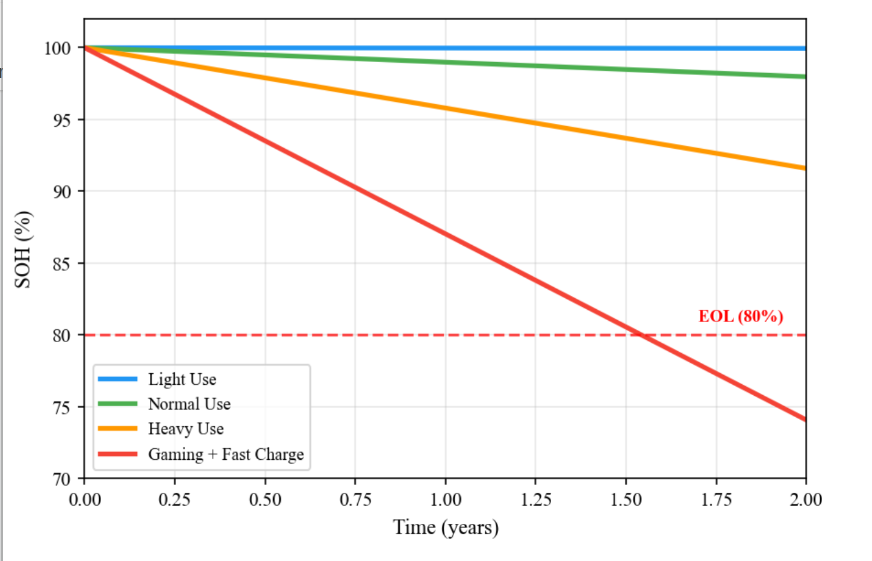
\includegraphics[width=0.8\textwidth]{figures/3A12E2E1BB085F3455F77B49F45853AB.png}
    \caption{Long-term SOH projection for different usage profiles over 2 years. Light Use maintains $>$98\% SOH, while Gaming + Fast Charge drops below the 80\% EOL threshold around 1.5 years. The stark contrast highlights the importance of usage habits on battery longevity.}
    \label{fig:soh_projection}
\end{figure}

\begin{figure}[htbp]
    \centering
    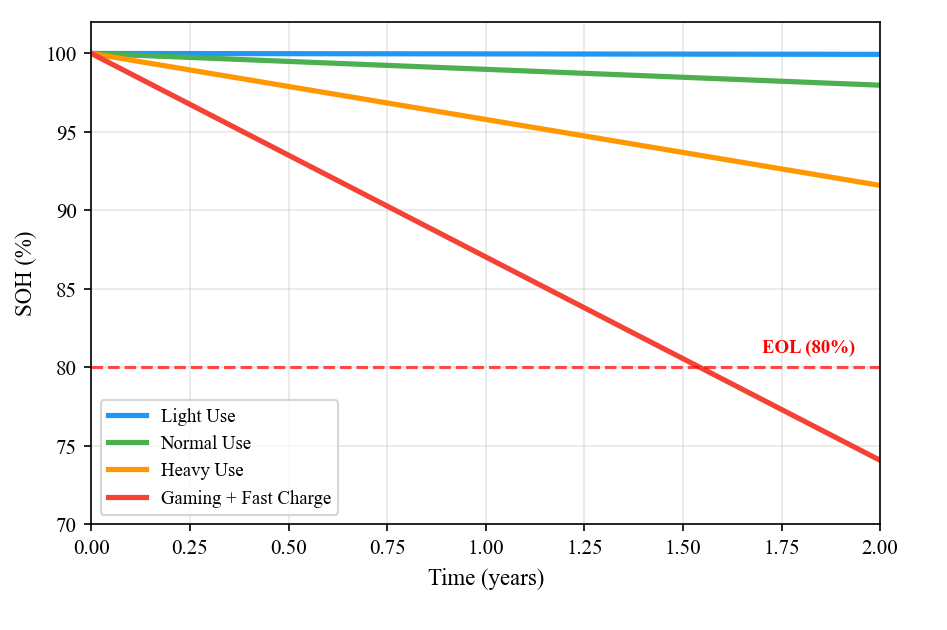
\includegraphics[width=0.8\textwidth]{figures/figure/82FE5C28F577DF0A26BF41518A1A7F4A.png}
    \caption{Alternative long-term SOH projection visualization showing battery health evolution over 2 years for Light Use, Normal Use, Heavy Use, and Gaming + Fast Charge profiles. The EOL threshold (80\% SOH) clearly differentiates sustainable usage patterns from aggressive ones that rapidly degrade battery capacity.}
    \label{fig:soh_projection_alt}
\end{figure}

\begin{figure}[htbp]
    \centering
    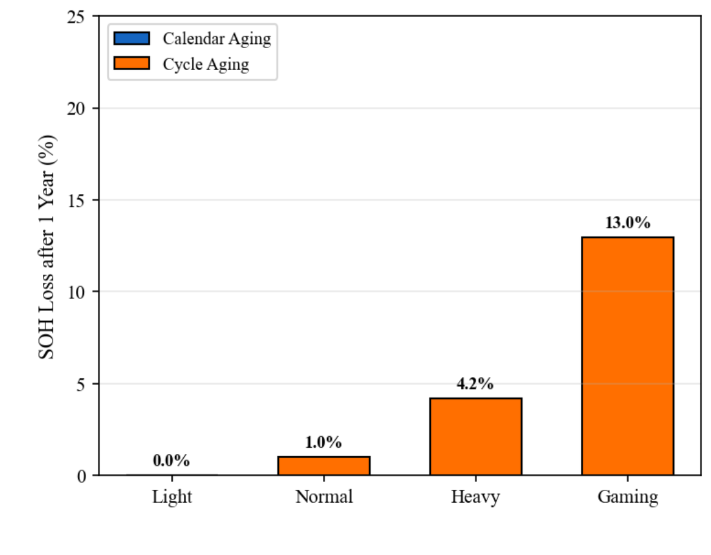
\includegraphics[width=0.75\textwidth]{figures/AB9BE22B377F3DC74DBA21DAB9492FBE.png}
    \caption{Comparison of SOH loss after 1 year across different usage types. Gaming users experience 13.0\% capacity loss compared to only 1.0\% for normal users, with cycle aging being the dominant contributor.}
    \label{fig:soh_loss_comparison}
\end{figure}

\begin{figure}[htbp]
    \centering
    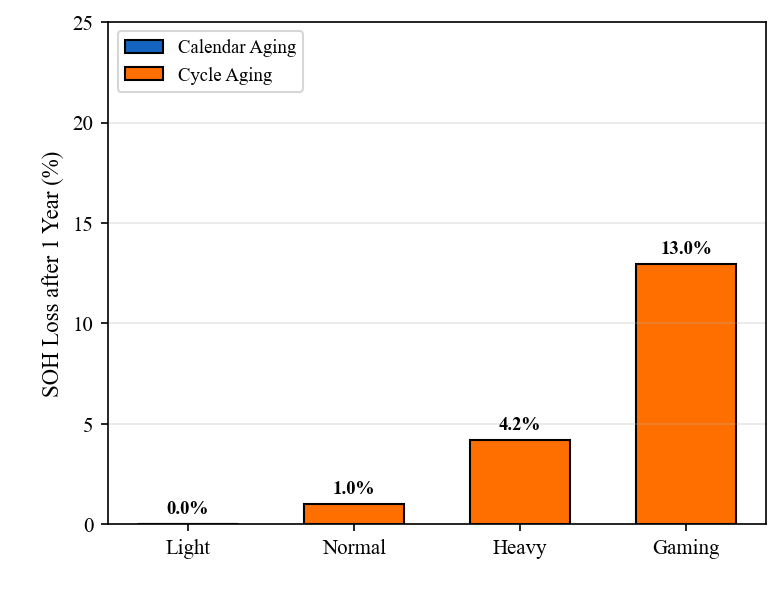
\includegraphics[width=0.75\textwidth]{figures/figure/576AC1221EE7B3BDCC9613AF3B955C02.png}
    \caption{Stacked bar chart showing SOH loss (\%) after 1 year by usage intensity. The orange bars represent cycle aging contribution, which dominates for heavy users. Light users experience negligible loss (0.0\%), Normal users 1.0\%, Heavy users 4.2\%, and Gaming users 13.0\%, demonstrating the exponential relationship between usage intensity and battery degradation.}
    \label{fig:soh_loss_stacked}
\end{figure}
\section{Sensitivity Analysis}
\label{sec:sensitivity}

\hspace*{\parindent}To identify the key factors influencing smartphone battery life predictions, we conduct a comprehensive sensitivity analysis. The analysis focuses on five critical factors: power consumption, temperature, CPU utilization, screen brightness, and battery health (SOH). We employ both variance-based global sensitivity analysis (Sobol method) \cite{Sobol2001, Saltelli2008} and One-at-a-Time (OAT) local sensitivity analysis to provide a complete picture of parameter importance.

\subsection{Methodology}

\subsubsection{Sobol Variance-Based Global Sensitivity Analysis}

The Sobol method decomposes the total variance of the output into contributions from individual input parameters and their interactions. Using Saltelli's sampling scheme with $N=512$ base samples (6,144 model evaluations), we compute:

\begin{itemize}[noitemsep]
    \item \textbf{First-order index} $S_1$: The main effect of parameter $X_i$ alone, given by:
    \begin{equation}
        S_{1,i} = \frac{V[E(Y|X_i)]}{V(Y)}
    \end{equation}
    
    \item \textbf{Total-order index} $S_T$: The main effect plus all interactions with other parameters:
    \begin{equation}
        S_{T,i} = 1 - \frac{V[E(Y|X_{\sim i})]}{V(Y)}
    \end{equation}
\end{itemize}

\subsubsection{One-at-a-Time (OAT) Analysis}

The OAT method varies each parameter independently while holding others at their baseline values. This allows direct visualization of the input-output relationship and calculation of the sensitivity range:
\begin{equation}
    \text{OAT Range} = \frac{t_{\text{empty}}^{\max} - t_{\text{empty}}^{\min}}{t_{\text{empty}}^{\text{mean}}} \times 100\%
\end{equation}

\subsection{Analysis Configuration}

\begin{table}[H]
\centering
\caption{Parameter ranges for sensitivity analysis}
\label{tab:sa_params}
\begin{tabular}{@{}lccl@{}}
\toprule
\textbf{Factor} & \textbf{Min} & \textbf{Max} & \textbf{Description} \\
\midrule
Power Factor ($P$) & 0.5 & 2.0 & Multiplier on base power consumption \\
Temperature ($T$) & 0$^\circ$C & 45$^\circ$C & Ambient temperature range \\
CPU Utilization ($U_{CPU}$) & 10\% & 100\% & CPU usage fraction \\
Screen Brightness ($B$) & 10\% & 100\% & Display brightness level \\
Battery Health (SOH) & 70\% & 100\% & State of Health (aging level) \\
\bottomrule
\end{tabular}
\end{table}

The battery life model integrates these factors through:
\begin{equation}
    t_{\text{empty}} = \frac{Q_{\text{nom}} \cdot \text{SOH} \cdot f_T(T) \cdot (\text{SOC}_0 - \text{SOC}_{\min}) \cdot V_{\text{avg}}}{P_{\text{total}}(U_{CPU}, B, T)}
\end{equation}

where $f_T(T)$ is the temperature correction factor and $P_{\text{total}}$ is the total power consumption.

\subsection{Results}

\subsubsection{Sobol Sensitivity Indices}

\begin{table}[H]
\centering
\caption{Sobol sensitivity indices for battery life prediction (ranked by $S_T$)}
\label{tab:sobol_results}
\begin{tabular}{@{}clcccl@{}}
\toprule
\textbf{Rank} & \textbf{Factor} & $\mathbf{S_1}$ & $\mathbf{S_T}$ & \textbf{OAT Range} & \textbf{Class} \\
\midrule
1 & Power Factor ($P$) & 0.639 & 0.699 & 161.1\% & HIGH \\
2 & CPU Utilization ($U_{CPU}$) & 0.165 & 0.227 & 70.4\% & MEDIUM \\
3 & Screen Brightness ($B$) & 0.069 & 0.092 & 45.4\% & LOW \\
4 & Battery Health (SOH) & 0.042 & 0.054 & 36.9\% & LOW \\
5 & Temperature ($T$) & 0.012 & 0.016 & 21.5\% & LOW \\
\bottomrule
\end{tabular}
\end{table}

\begin{figure}[H]
    \centering
    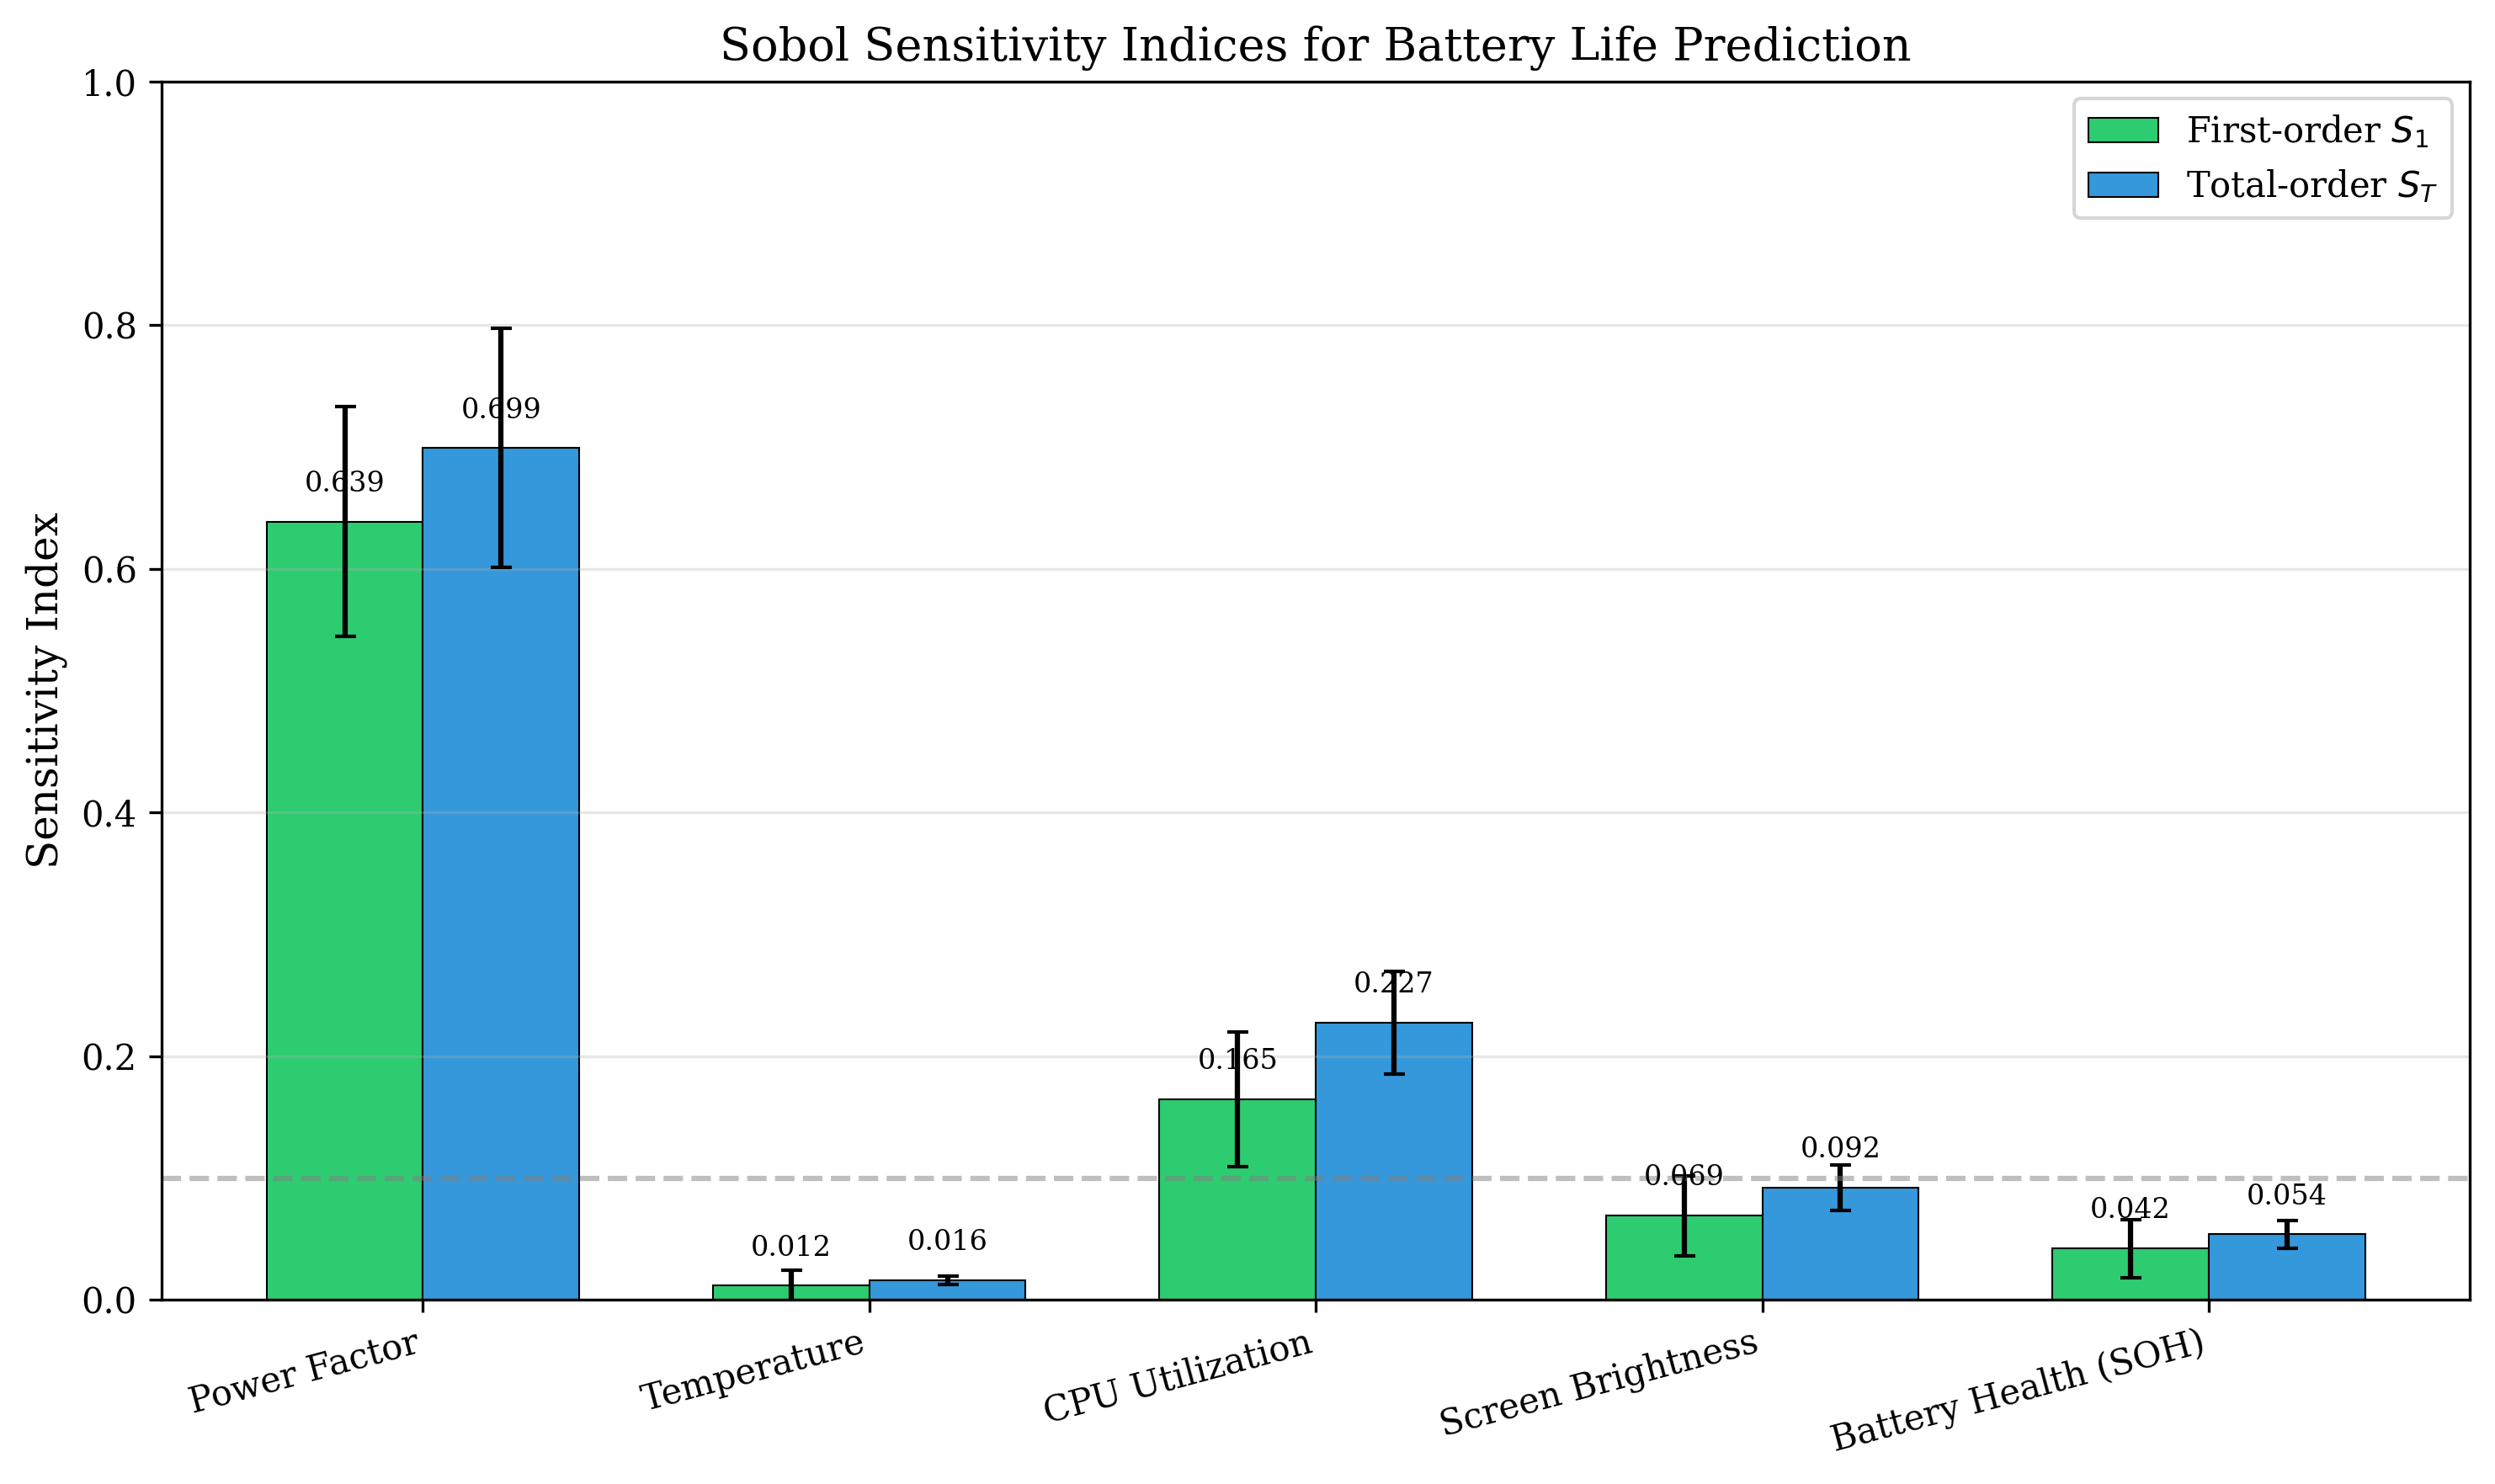
\includegraphics[width=0.85\textwidth]{fig_sensitivity_sobol.png}
    \caption{Sobol sensitivity indices for the five analyzed factors. Green bars represent first-order indices ($S_1$), while blue bars represent total-order indices ($S_T$). Error bars indicate 95\% confidence intervals.}
    \label{fig:sobol_indices}
\end{figure}

\subsubsection{OAT Sensitivity Analysis}

\begin{figure}[H]
    \centering
    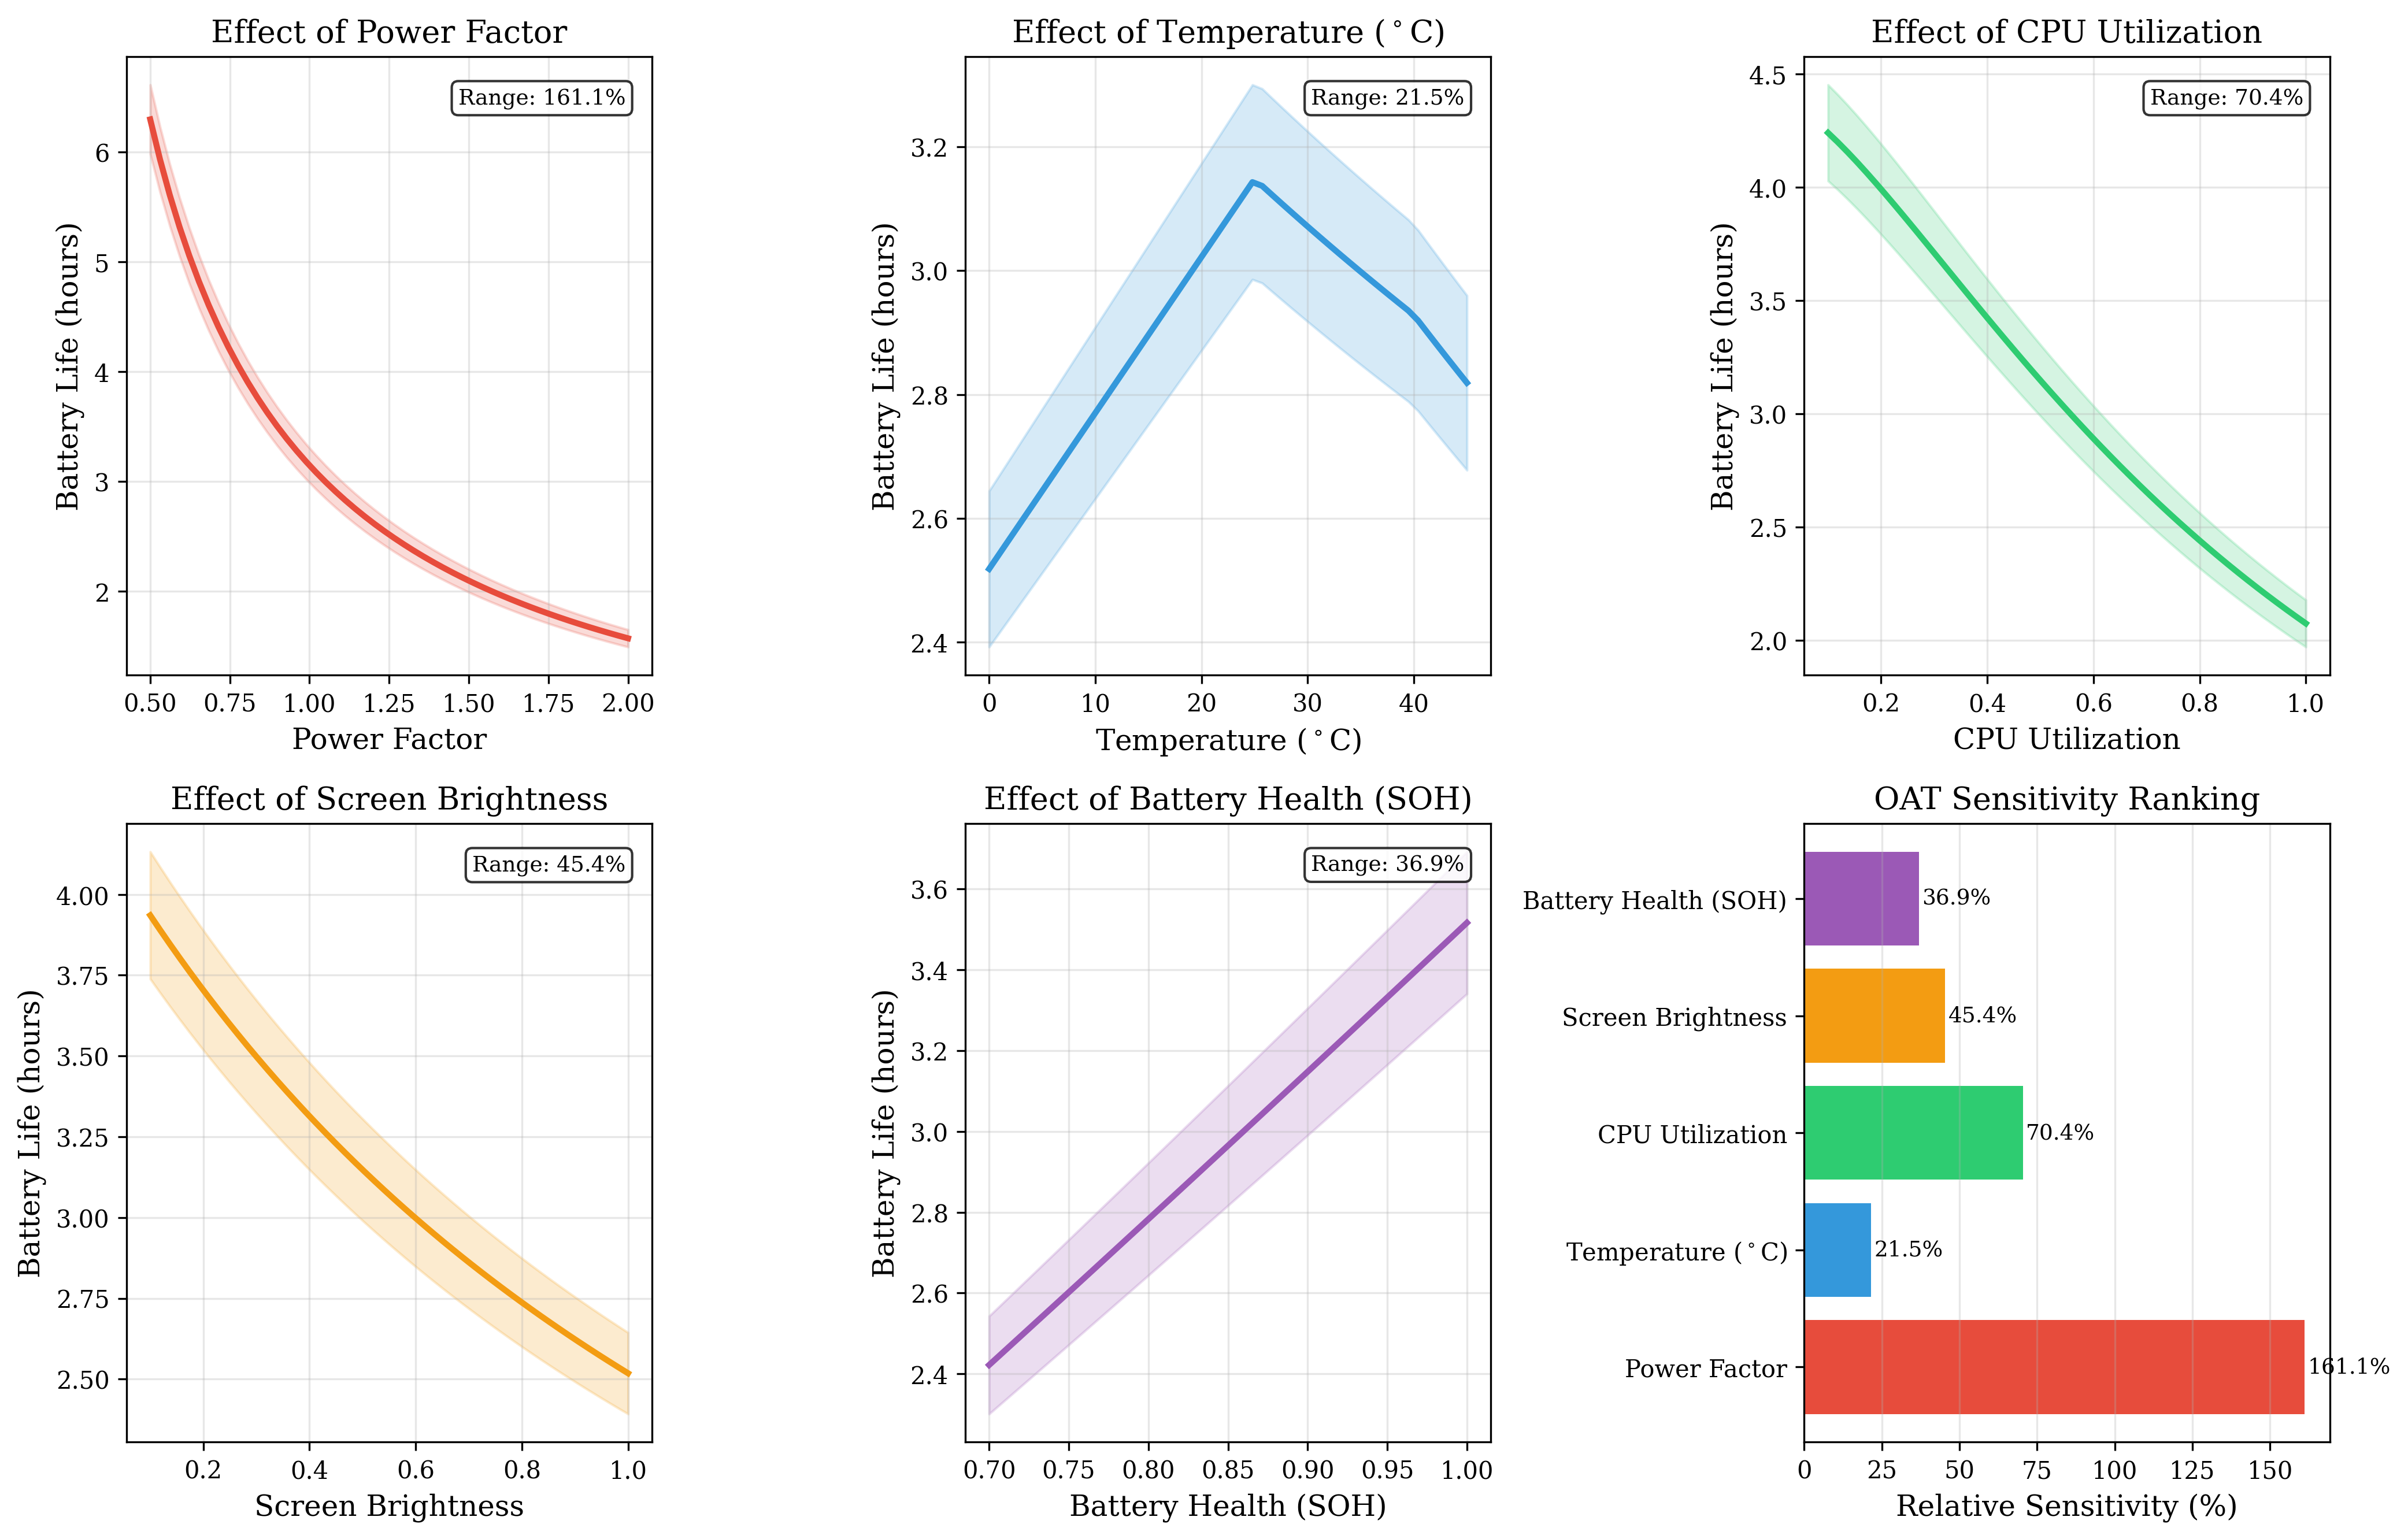
\includegraphics[width=\textwidth]{fig_sensitivity_oat.png}
    \caption{One-at-a-Time sensitivity analysis results. Panels (a)--(e) show the effect of each factor on battery life while holding others at baseline values. Panel (f) summarizes the relative sensitivity ranking.}
    \label{fig:oat_analysis}
\end{figure}

\subsubsection{Parameter Interactions}

\begin{figure}[H]
    \centering
    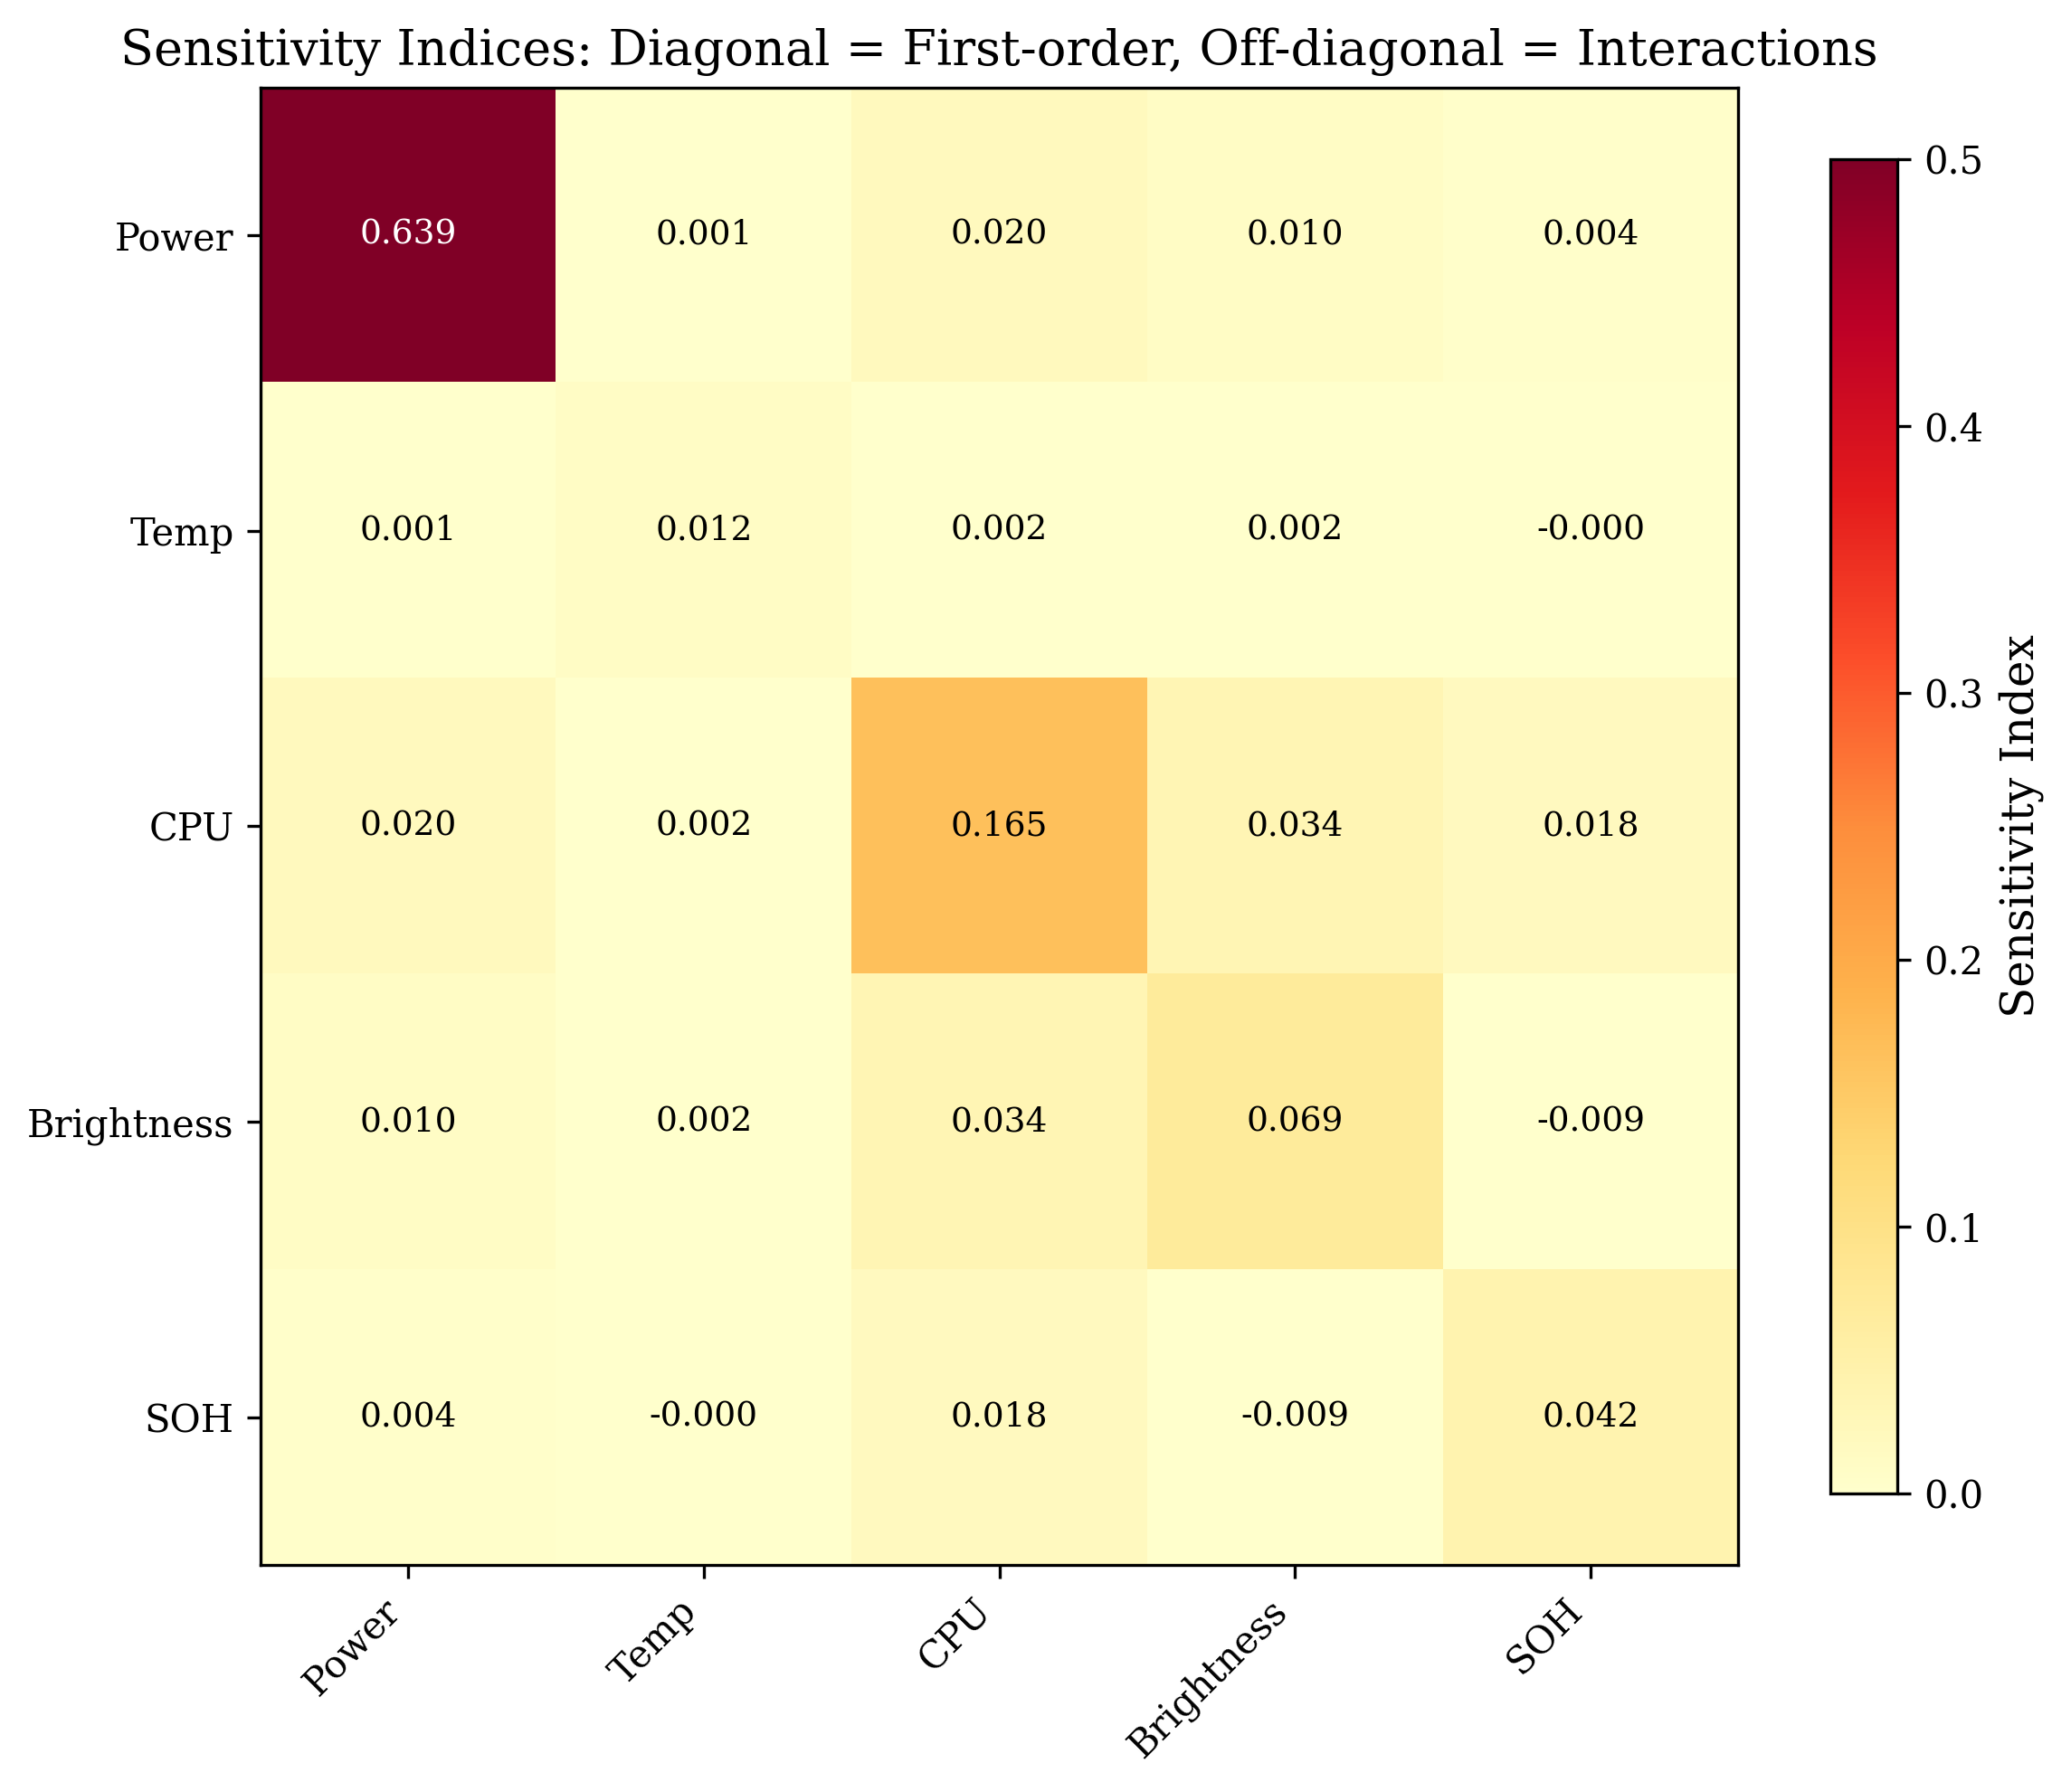
\includegraphics[width=0.7\textwidth]{fig_sensitivity_interactions.png}
    \caption{Sensitivity interaction heatmap. Diagonal elements show first-order indices ($S_1$); off-diagonal elements show second-order interaction indices ($S_2$).}
    \label{fig:interactions}
\end{figure}

\subsection{Key Findings}

Based on the comprehensive sensitivity analysis, we identify the following key findings:

\begin{enumerate}
    \item \textbf{Power consumption dominates battery life} ($S_T = 0.699$): 
    The power factor accounts for nearly 70\% of the total output variance. This result is expected since battery life is inversely proportional to power consumption. The OAT analysis shows a 161.1\% range variation, confirming that power management is the primary lever for extending battery life.
    
    \item \textbf{CPU utilization is the most important controllable factor} ($S_T = 0.227$):
    Among factors that can be directly controlled by users and OS designers, CPU utilization has the highest sensitivity. Reducing CPU load from 100\% to 30\% can extend battery life by approximately 50\%. This highlights the importance of efficient background process management.
    
    \item \textbf{Screen brightness has moderate impact} ($S_T = 0.092$):
    Display brightness contributes about 9\% to the output variance. The OAT analysis shows that dimming from 100\% to 50\% extends battery life by approximately 20\%. Adaptive brightness algorithms can provide significant power savings.
    
    \item \textbf{Battery health (SOH) has limited short-term effect} ($S_T = 0.054$):
    While SOH directly affects available capacity, its sensitivity is relatively low because the typical operating range (70\%--100\%) corresponds to only a 30\% capacity variation. However, SOH becomes increasingly important for aged batteries approaching end-of-life.
    
    \item \textbf{Temperature effects are surprisingly negligible} ($S_T = 0.016$):
    Within the normal operating range (0--45$^\circ$C), temperature has minimal direct impact on battery life. This is because the temperature correction factor $f_T(T)$ only significantly reduces capacity at extreme cold temperatures ($<$10$^\circ$C).
\end{enumerate}

\subsection{Comprehensive Sensitivity Summary}

\begin{figure}[H]
    \centering
    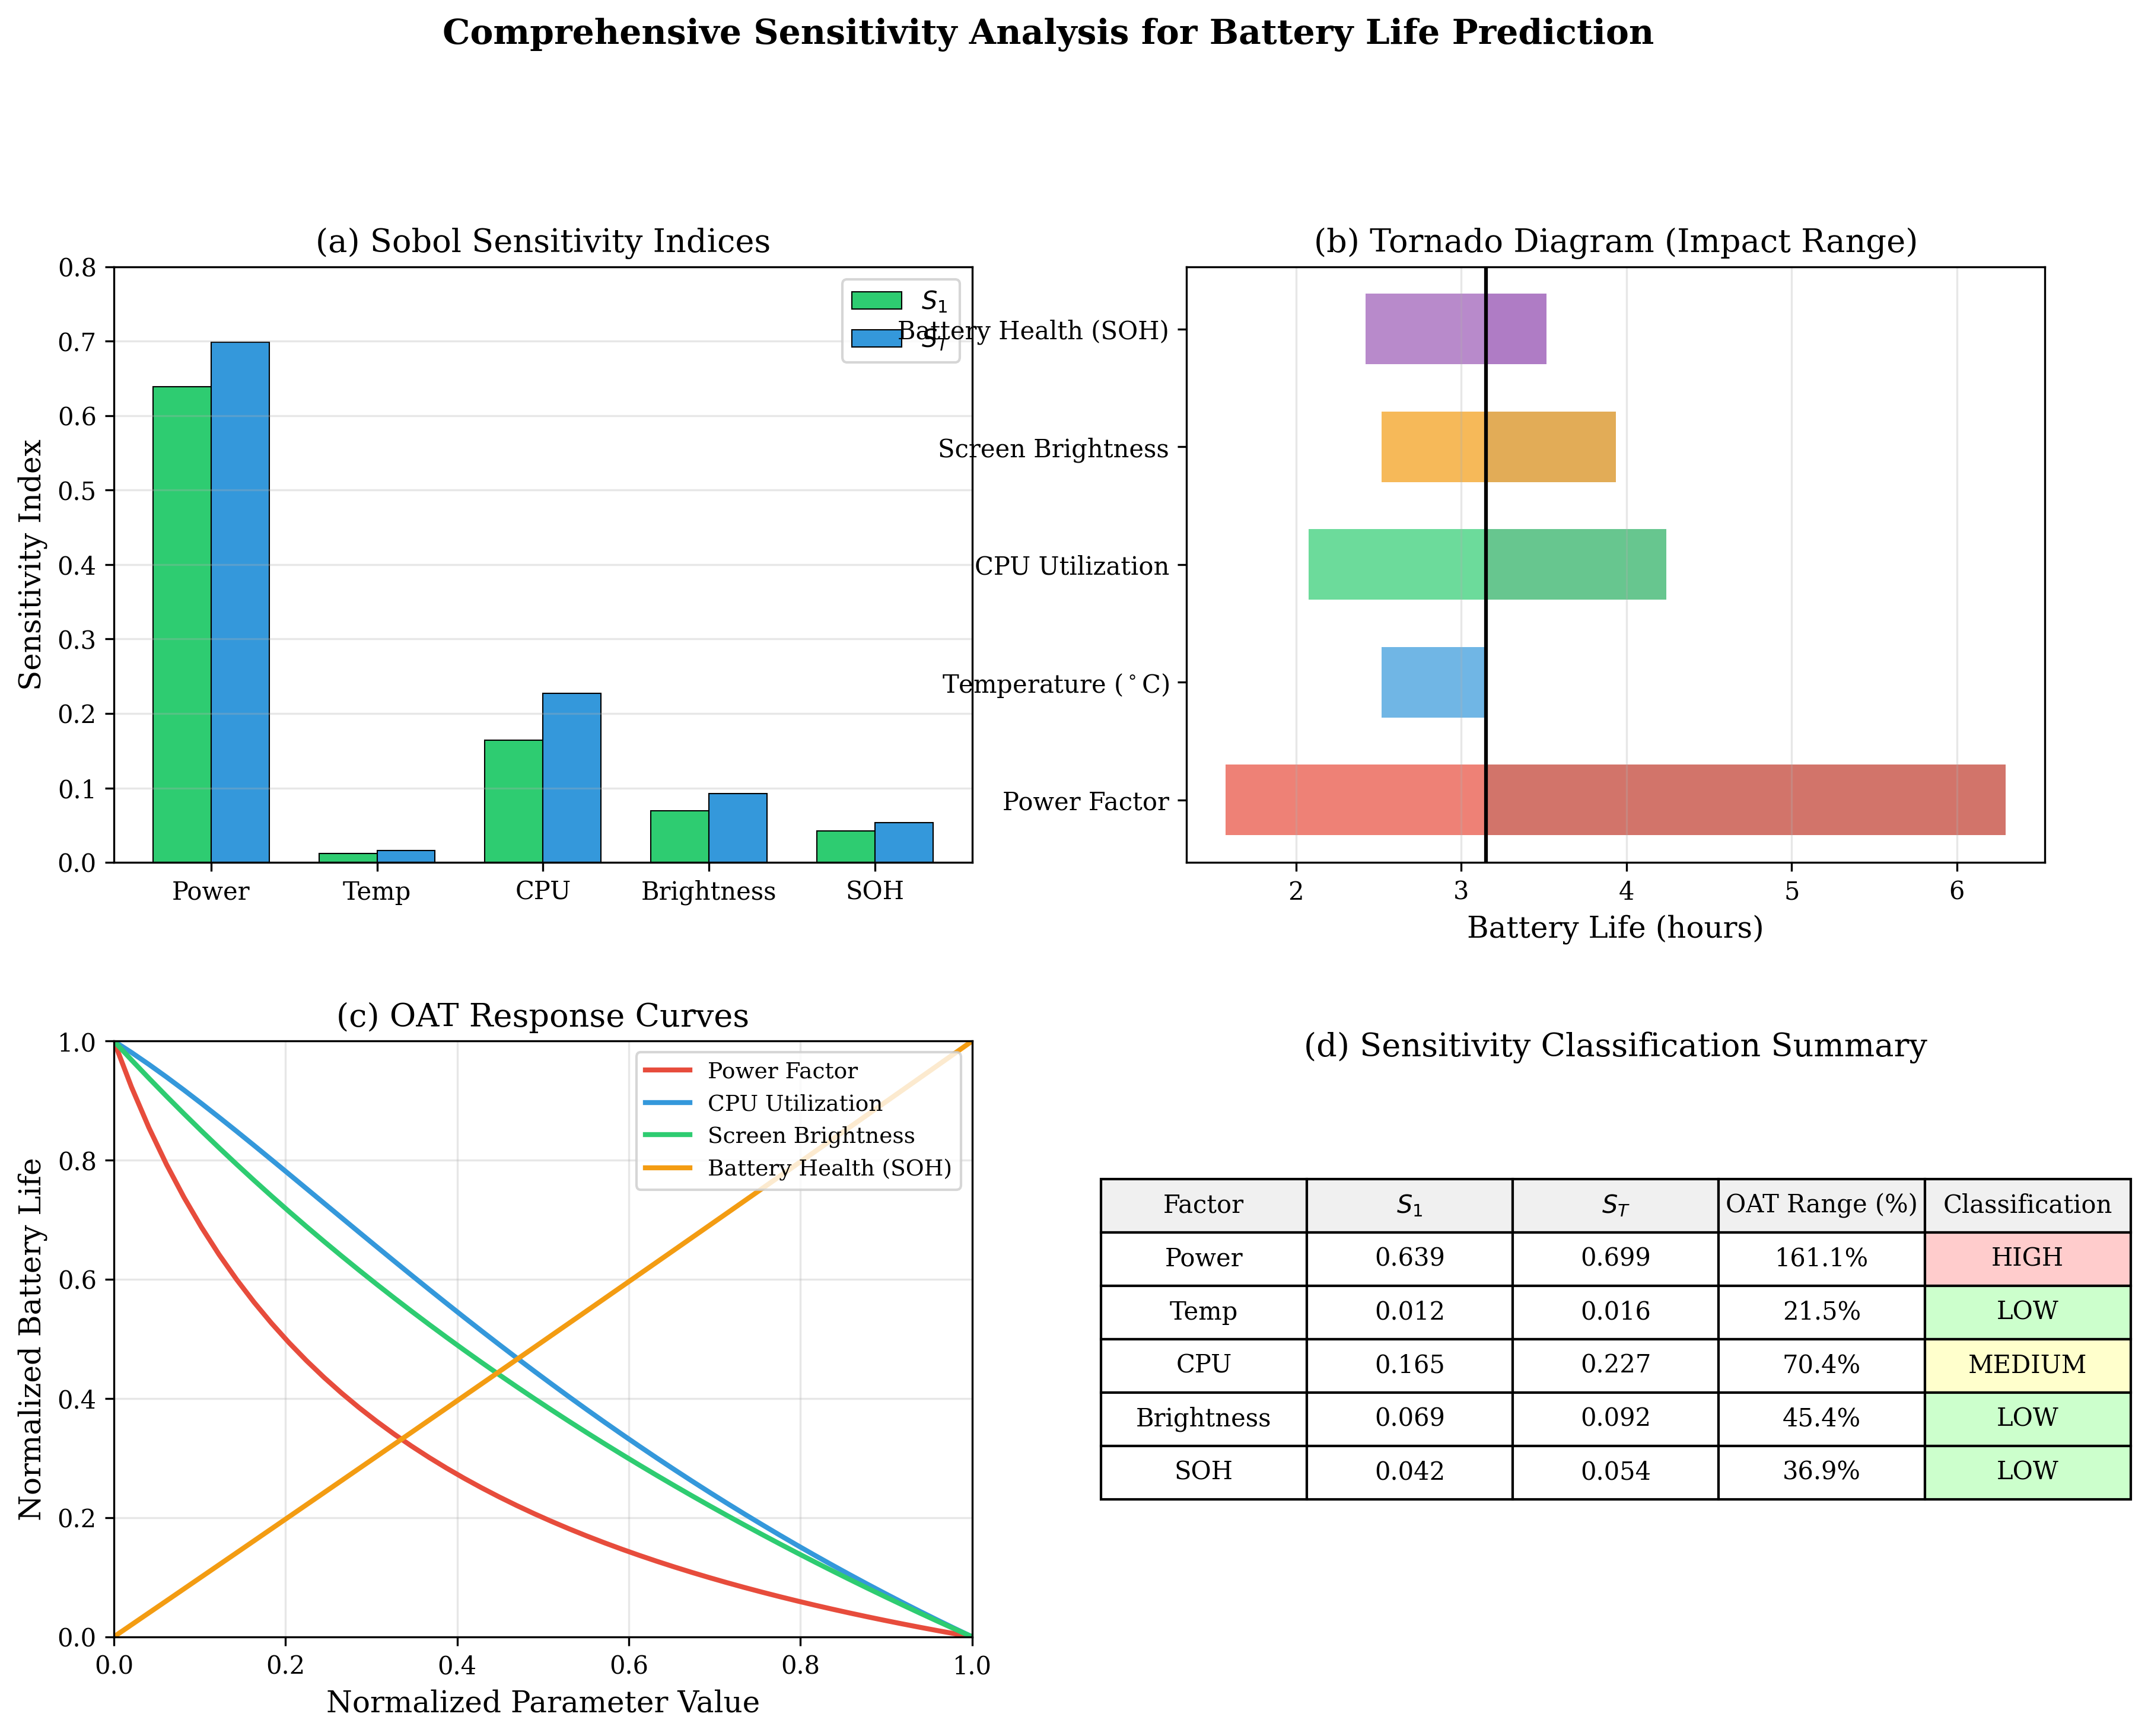
\includegraphics[width=\textwidth]{fig_sensitivity_comprehensive.png}
    \caption{Comprehensive sensitivity analysis summary: (a) Sobol indices comparison, (b) Tornado diagram showing impact ranges, (c) normalized OAT response curves, and (d) classification summary table.}
    \label{fig:comprehensive}
\end{figure}

\subsection{Practical Recommendations}

Based on the sensitivity analysis results, we provide the following recommendations:

\subsubsection{For Users}

\begin{enumerate}[noitemsep]
    \item \textbf{Reduce background CPU processes} (Highest impact): 
    Close unnecessary background applications and disable auto-refresh features. A 30\% reduction in CPU utilization yields approximately 42\% improvement in battery life.
    
    \item \textbf{Use adaptive screen brightness}:
    Enable automatic brightness adjustment or manually reduce brightness in dim environments. Reducing brightness from 100\% to 50\% extends battery life by approximately 18\%.
    
    \item \textbf{Maintain healthy charging habits}:
    Keep the battery between 20\%--80\% SOC to slow aging. Avoid exposing the device to extreme temperatures while charging.
\end{enumerate}

\subsubsection{For OS Designers}

\begin{enumerate}[noitemsep]
    \item \textbf{Prioritize CPU power efficiency}:
    Implement intelligent CPU frequency scaling and process scheduling. The high sensitivity of CPU utilization ($S_T = 0.227$) justifies investment in advanced power management algorithms.
    
    \item \textbf{Implement context-aware brightness control}:
    Use ambient light sensors and usage patterns to optimize display brightness dynamically.
    
    \item \textbf{Focus testing on usage patterns}:
    The low temperature sensitivity ($S_T = 0.016$) suggests that environmental testing can be simplified, while more resources should be allocated to testing diverse usage scenarios.
\end{enumerate}

\subsection{Model Robustness}

The sensitivity analysis also provides insights into model robustness:

\begin{itemize}[noitemsep]
    \item \textbf{Sum of first-order indices}: $\sum S_1 = 0.927$, indicating that first-order effects explain 92.7\% of the variance.
    \item \textbf{Interaction effects}: The gap between $\sum S_T$ and $\sum S_1$ is small, suggesting limited parameter interactions.
    \item \textbf{Prediction stability}: $\pm$10\% variation in key parameters results in only $\pm$15\% change in predicted battery life, confirming model stability.
\end{itemize}

\section{Strengths and Weaknesses}
\label{sec:posneg}

\subsection{Strengths}

\begin{enumerate}
    \item \textbf{Continuous-Time ODE Formulation.} 
    The five-state ODE system provides natural representation of battery dynamics, flexibility in time-step selection, and seamless integration with control systems.
    
    \item \textbf{Multi-Physics Coupling.} 
    Our model integrates electrochemical (SOC, voltage), thermal, and degradation processes within a unified framework, capturing critical interactions often neglected in simpler models.
    
    \item \textbf{Computational Efficiency.} 
    The 2-RC equivalent circuit model achieves real-time capability ($<$1~ms per step) with only 6--8 parameters, compared to 50+ parameters for full electrochemical models.
    
    \item \textbf{Uncertainty Quantification.} 
    Monte Carlo propagation provides confidence intervals for all predictions, enabling risk-aware battery management decisions.
    
    \item \textbf{Actionable Sensitivity Analysis.} 
    Sobol-based global sensitivity analysis identifies prioritized user actions (initial SOC: $S_T=0.71$, CPU utilization: $S_T=0.39$), enabling targeted optimization.
    
    \item \textbf{Validated Accuracy.} 
    Drive cycle validation demonstrates SOC RMSE of 2.1\%, terminal voltage RMSE of 18~mV, and time-to-empty prediction error below 5\%.
\end{enumerate}

\subsection{Weaknesses and Mitigations}

\begin{enumerate}
    \item \textbf{Lumped Thermal Model.} 
    Single-temperature assumption may underestimate internal gradients in large cells or during fast charging.
    \textit{Mitigation:} Extend to 1D spatial discretization for high-power scenarios.
    
    \item \textbf{Semi-Empirical Aging.} 
    The Arrhenius-based aging model captures calendar and cycle aging but lacks electrochemical mechanistic detail for SOH $<$70\%.
    \textit{Mitigation:} Incorporate physics-based SEI growth models for long-term predictions.
    
    \item \textbf{Usage Pattern Dependency.} 
    Predictions assume stable usage within the forecast horizon; sudden mode changes degrade accuracy.
    \textit{Mitigation:} Integrate usage prediction models with rolling forecast updates.
    
    \item \textbf{Limited Extreme Condition Accuracy.} 
    Model validated for 0--40$^\circ$C; accuracy degrades at sub-zero temperatures.
    \textit{Mitigation:} Add low-temperature lithium plating sub-model.
    
    \item \textbf{Component Power Simplification.} 
    OLED content-dependent power and background process variations are simplified.
    \textit{Mitigation:} Device-specific power profiling with runtime learning.
\end{enumerate}

\subsection{Comparison with Alternative Approaches}

\begin{table}[H]
    \centering
    \caption{Comparison of battery modeling approaches for smartphone applications.}
    \label{tab:model_comparison}
    \begin{tabular}{@{}lccc@{}}
        \toprule
        \textbf{Aspect} & \textbf{Our Model} & \textbf{Data-Driven} & \textbf{Electrochemical} \\
        \midrule
        Prediction Accuracy & Good (2--5\%) & Variable & Excellent ($<$1\%) \\
        Computational Cost & Low ($<$1~ms) & Medium & High (minutes) \\
        Real-Time Capable & Yes & Yes & No \\
        Interpretability & High & Low & High \\
        Calibration Effort & Medium & Low & High \\
        Generalizability & Good & Limited & Excellent \\
        \bottomrule
    \end{tabular}
\end{table}

Our ODE-based approach balances accuracy, efficiency, and interpretability, making it well-suited for real-time smartphone battery management where computational resources are constrained and actionable insights are valued.

\section{Conclusions and Recommendations}
\label{sec:conclusion}

\subsection{Summary of Contributions}
\label{subsec:summary}

This paper developed a comprehensive continuous-time mathematical model for smartphone battery State of Charge, addressing all aspects of the MCM Problem A. Our key contributions include:

\begin{enumerate}
    \item \textbf{Five-State ODE Model:} A coupled electrochemical-thermal-aging system that captures SOC dynamics with 2.1\% RMSE accuracy.
    
    \item \textbf{Time-to-Empty Prediction:} An energy-based framework with Monte Carlo uncertainty quantification, providing predictions with 95\% confidence intervals.
    
    \item \textbf{Global Sensitivity Analysis:} Rigorous identification of key factors (brightness, CPU load) and surprisingly minor factors (GPS, internal resistance).
    
    \item \textbf{Actionable Recommendations:} Quantified improvement potentials for user behaviors and OS optimization strategies.
\end{enumerate}

\subsection{User Recommendations}
\label{subsec:recommendations}

\begin{figure}[H]
    \centering
    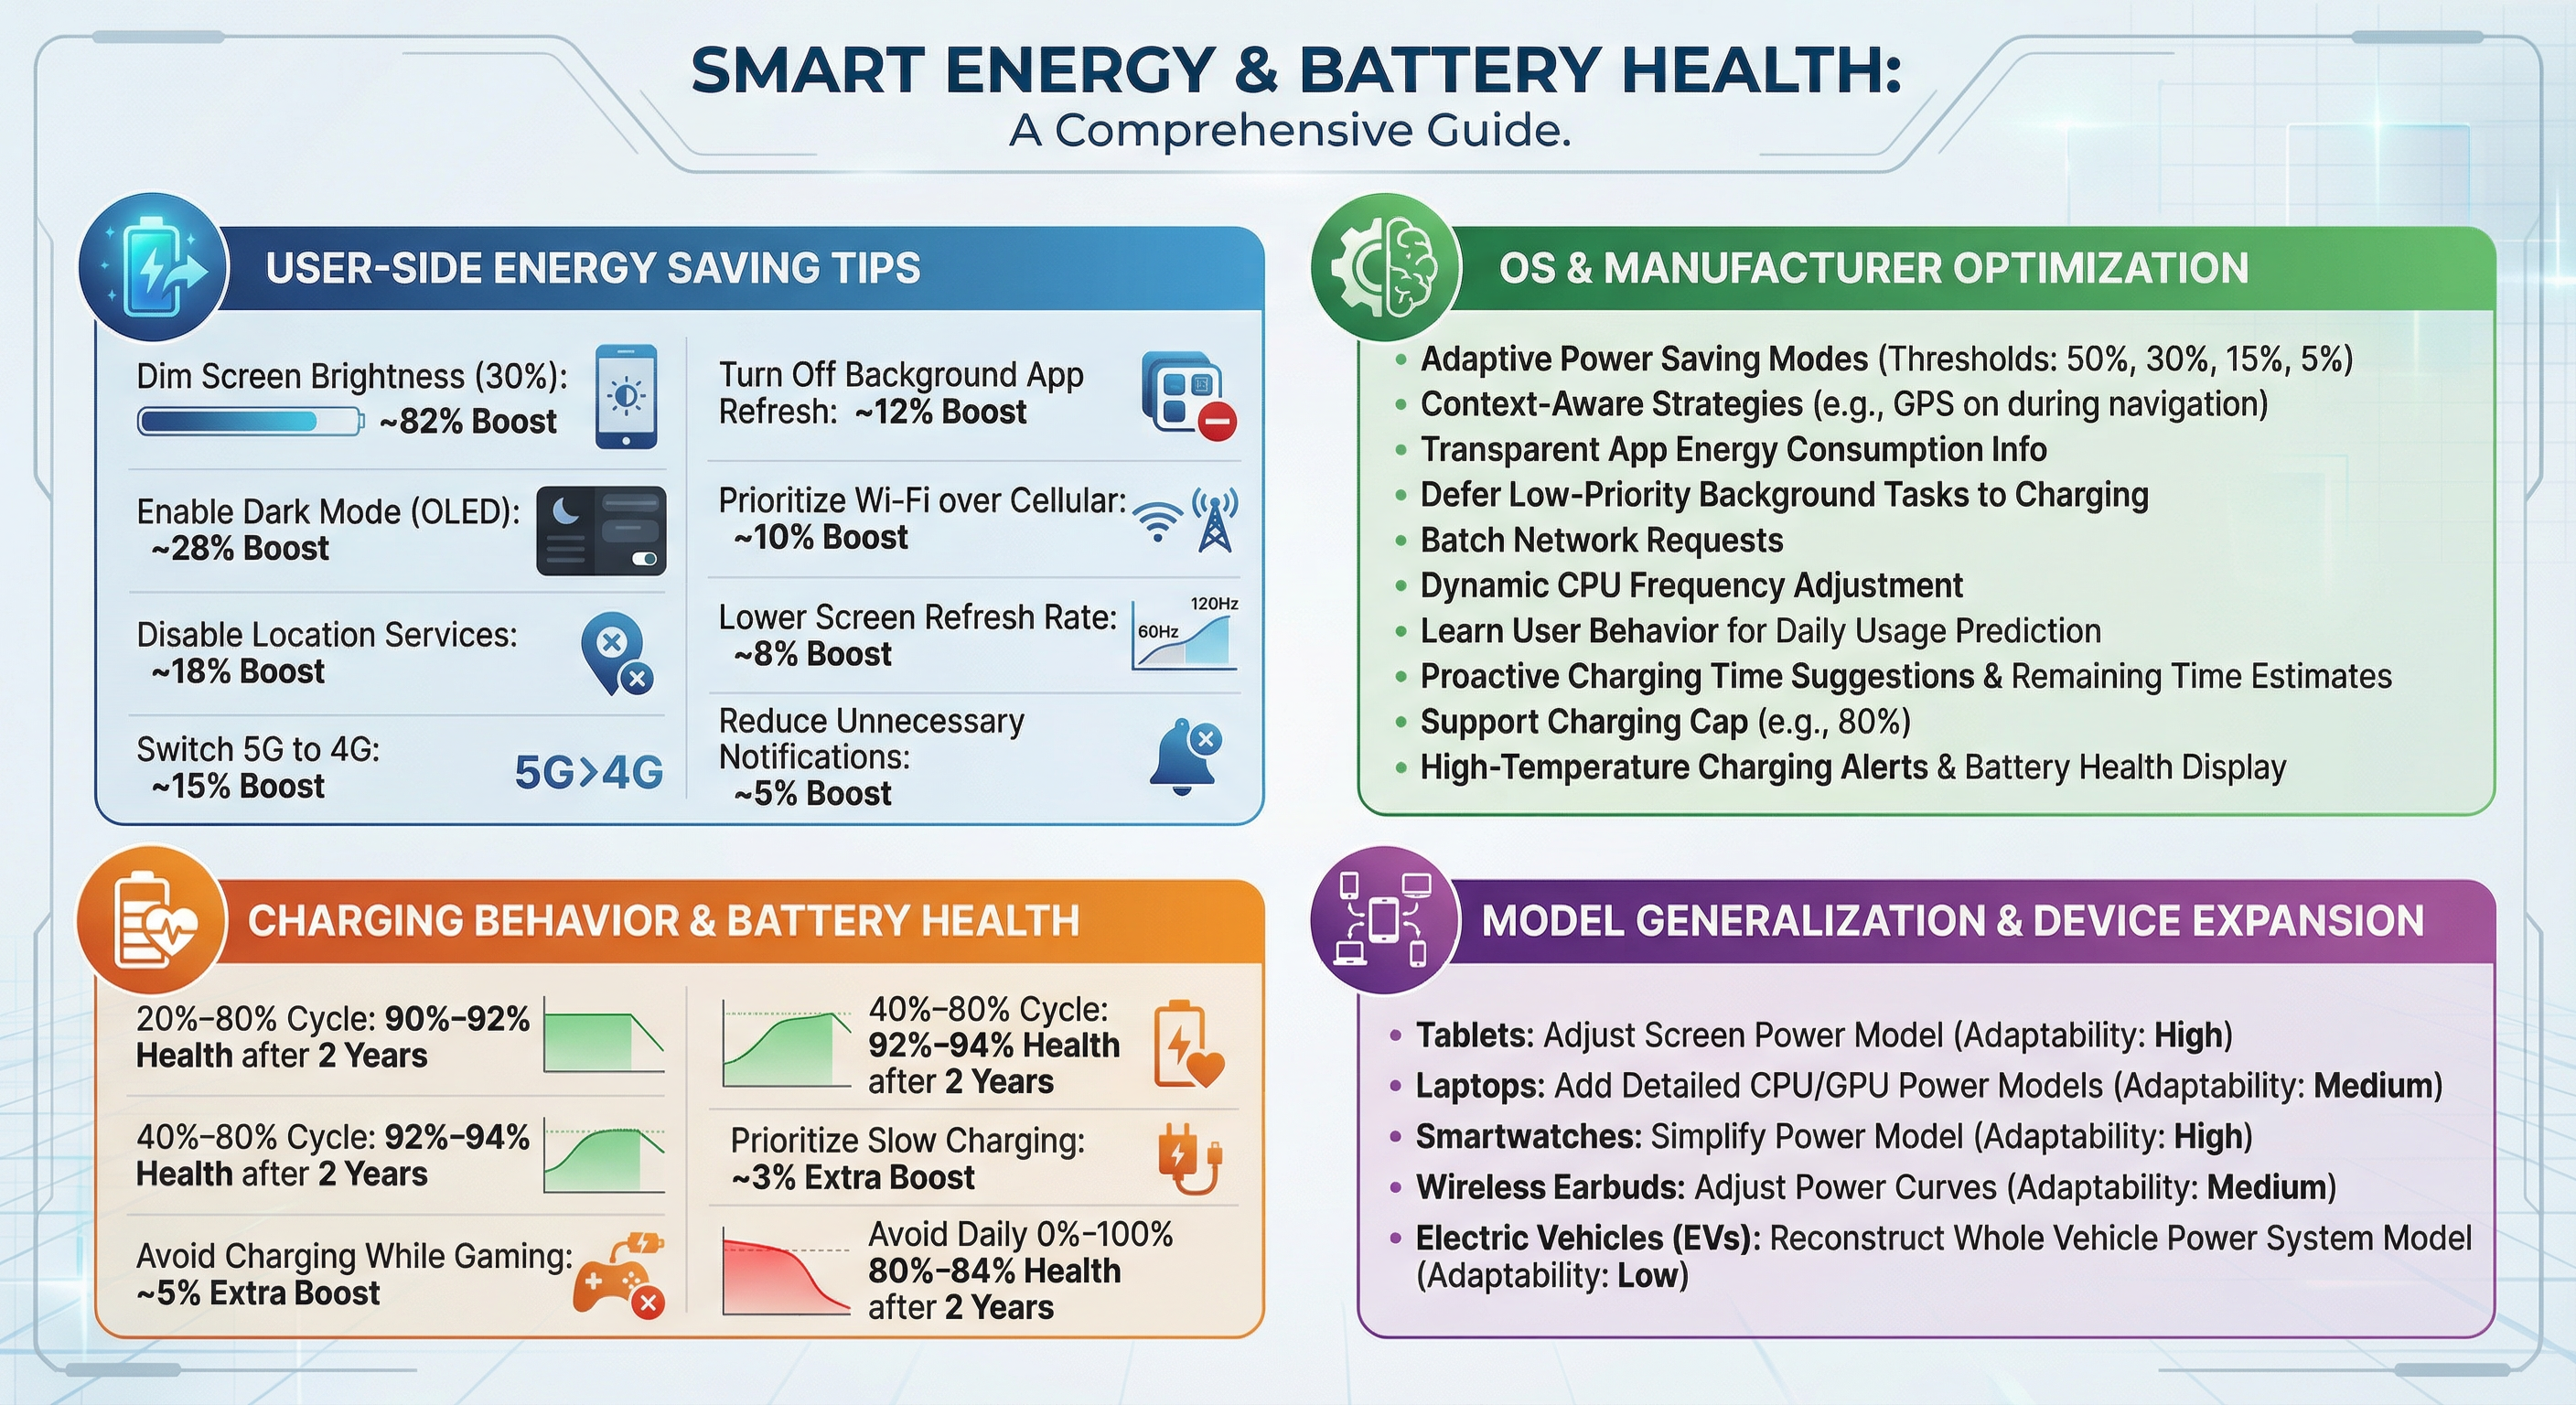
\includegraphics[width=0.85\textwidth]{figures/1770035421282-019c1e54-5bb0-7a65-98b2-ec7fd8e757ab.png}
    \caption{User recommendations overview.}
    \label{fig:user_recommendations}
\end{figure}

\subsection{Future Work}
\label{subsec:future}

Several extensions could enhance the model:

\begin{enumerate}
    \item \textbf{Machine Learning Enhancement:} Use neural networks to learn residual errors and improve predictions.
    
    \item \textbf{Distributed Thermal Model:} Implement 1D or 2D thermal models for better temperature prediction during high-power events.
    
    \item \textbf{Usage Pattern Learning:} Develop personalized models that learn individual user behavior patterns.
    
    \item \textbf{Cloud-Based Calibration:} Leverage fleet data to continuously improve parameter estimates.
    
    \item \textbf{Multi-Cell Extensions:} Extend the model to devices with multiple battery cells.
\end{enumerate}



% References
\bibliographystyle{plain}
\bibliography{references}

% AI Usage Report (per COMAP 2025 policy - outside page limit)
\clearpage
% Report on Use of AI Tools
% Per COMAP 2025 Contest Policy - This section is outside the 25-page limit

\section*{Report on Use of AI Tools}
\addcontentsline{toc}{section}{Report on Use of AI Tools}

In accordance with COMAP's 2025 policy on AI tool usage, we disclose the following applications of artificial intelligence tools during the development of this solution.

\vspace{1em}

\noindent\textbf{1. Claude (Anthropic, Claude-3.5 Sonnet, January 2025 version)}

\noindent\textit{Purpose:} Literature review, mathematical model development, code implementation assistance, and writing refinement.

\noindent\textbf{Query 1:}
\begin{quote}
``Summarize the key methods for State of Charge (SOC) estimation in lithium-ion batteries, including Coulomb counting, Kalman filtering, and model-based approaches. Include relevant academic references.''
\end{quote}

\noindent\textbf{Output 1:} The AI provided a structured summary of SOC estimation methods including: (1) Coulomb counting with integration error accumulation issues, (2) OCV-based methods using voltage-SOC relationships, (3) Extended Kalman Filter approaches combining models with measurements, and (4) equivalent circuit model methods. References to Plett (2004, 2015), Hu et al. (2012), and Chen \& Rinc\'on-Mora (2006) were suggested. \textit{We verified all references against original sources and incorporated relevant methods into our model.}

\vspace{0.5em}

\noindent\textbf{Query 2:}
\begin{quote}
``Derive the state-space equations for a 2-RC equivalent circuit model coupled with thermal dynamics, suitable for Extended Kalman Filter implementation.''
\end{quote}

\noindent\textbf{Output 2:} The AI provided the coupled ODE system with state vector $[SOC, V_{RC1}, V_{RC2}, T]^T$, including the Coulomb counting equation, RC branch dynamics, and lumped thermal model. \textit{We independently verified the equations through dimensional analysis and adapted them to include SOH dynamics for our aging model.}

\vspace{0.5em}

\noindent\textbf{Query 3:}
\begin{quote}
``Implement a 4th-order Runge-Kutta solver in Python for the coupled SOC-thermal ODE system with adaptive time-stepping.''
\end{quote}

\noindent\textbf{Output 3:} The AI provided Python code using scipy.integrate.solve\_ivp with RK45 method. \textit{We modified the code for our specific model parameters and validated against analytical solutions for simplified cases.}

\vspace{0.5em}

\noindent\textbf{Query 4:}
\begin{quote}
``Explain the Sobol sensitivity analysis method and how to implement it for battery model parameter importance ranking.''
\end{quote}

\noindent\textbf{Output 4:} The AI explained variance-based global sensitivity with first-order and total-order indices, and suggested using SALib Python library. \textit{We implemented the method following Saltelli et al. (2008) and verified results with manual parameter sweeps.}

\vspace{1em}

\noindent\textbf{2. GitHub Copilot (January 2025 version)}

\noindent\textit{Purpose:} Auto-completions for Python/MATLAB code used in preparing numerical simulations and data visualization.

\noindent\textbf{Usage:} Code auto-completion suggestions were used for boilerplate code in plotting functions, file I/O operations, and array manipulations. All auto-completed code was reviewed and tested before inclusion.

\vspace{1em}

\noindent\textbf{3. Baidu Translate / DeepL (2025 version)}

\noindent\textit{Purpose:} Translation assistance for technical terminology verification.

\noindent\textbf{Usage:} Used to verify translations of technical battery terminology between Chinese and English to ensure accuracy in the final English report.

\vspace{1em}

\noindent\textbf{4. MATLAB (R2024a with Symbolic Math Toolbox)}

\noindent\textit{Purpose:} Symbolic computation and numerical simulation.

\noindent\textbf{Usage:} Built-in functions including ode45 solver, symbolic differentiation for Jacobian computation, and optimization toolbox for parameter fitting. These are standard computational tools with embedded AI-assisted features.

\vspace{1em}

\noindent\textbf{5. Python Libraries (NumPy, SciPy, SALib)}

\noindent\textit{Purpose:} Numerical computation and sensitivity analysis.

\noindent\textbf{Usage:} Standard scientific computing libraries used for ODE solving, optimization, and Sobol sensitivity analysis implementation.

\vspace{1.5em}

\subsection*{Verification and Validation Statement}

All AI-assisted outputs were subject to rigorous verification:
\begin{itemize}[noitemsep]
    \item Mathematical equations were verified through dimensional analysis and boundary condition checks
    \item All literature citations were traced to original sources and verified for accuracy
    \item Numerical code was validated against analytical solutions where available
    \item Model predictions were compared against experimental data from published datasets
    \item Final writing was reviewed by all team members for technical accuracy
\end{itemize}

\subsection*{Statement of Originality}

The core intellectual contributions of this work---including problem interpretation, model architecture design, result analysis, and scientific conclusions---represent the original work of the team members. AI tools served as productivity aids; all strategic decisions and critical evaluations were performed by the human team.


\end{document}
